
\documentclass{article} % For LaTeX2e
\usepackage{iclr2024_conference_preprint,times}

% Optional math commands from https://github.com/goodfeli/dlbook_notation.
%%%%% NEW MATH DEFINITIONS %%%%%

\usepackage{amsmath,amsfonts,bm}

% Mark sections of captions for referring to divisions of figures
\newcommand{\figleft}{{\em (Left)}}
\newcommand{\figcenter}{{\em (Center)}}
\newcommand{\figright}{{\em (Right)}}
\newcommand{\figtop}{{\em (Top)}}
\newcommand{\figbottom}{{\em (Bottom)}}
\newcommand{\captiona}{{\em (a)}}
\newcommand{\captionb}{{\em (b)}}
\newcommand{\captionc}{{\em (c)}}
\newcommand{\captiond}{{\em (d)}}

% Highlight a newly defined term
\newcommand{\newterm}[1]{{\bf #1}}


% Figure reference, lower-case.
\def\figref#1{figure~\ref{#1}}
% Figure reference, capital. For start of sentence
\def\Figref#1{Figure~\ref{#1}}
\def\twofigref#1#2{figures \ref{#1} and \ref{#2}}
\def\quadfigref#1#2#3#4{figures \ref{#1}, \ref{#2}, \ref{#3} and \ref{#4}}
% Section reference, lower-case.
\def\secref#1{section~\ref{#1}}
% Section reference, capital.
\def\Secref#1{Section~\ref{#1}}
% Reference to two sections.
\def\twosecrefs#1#2{sections \ref{#1} and \ref{#2}}
% Reference to three sections.
\def\secrefs#1#2#3{sections \ref{#1}, \ref{#2} and \ref{#3}}
% Reference to an equation, lower-case.
\def\eqref#1{equation~\ref{#1}}
% Reference to an equation, upper case
\def\Eqref#1{Equation~\ref{#1}}
% A raw reference to an equation---avoid using if possible
\def\plaineqref#1{\ref{#1}}
% Reference to a chapter, lower-case.
\def\chapref#1{chapter~\ref{#1}}
% Reference to an equation, upper case.
\def\Chapref#1{Chapter~\ref{#1}}
% Reference to a range of chapters
\def\rangechapref#1#2{chapters\ref{#1}--\ref{#2}}
% Reference to an algorithm, lower-case.
\def\algref#1{algorithm~\ref{#1}}
% Reference to an algorithm, upper case.
\def\Algref#1{Algorithm~\ref{#1}}
\def\twoalgref#1#2{algorithms \ref{#1} and \ref{#2}}
\def\Twoalgref#1#2{Algorithms \ref{#1} and \ref{#2}}
% Reference to a part, lower case
\def\partref#1{part~\ref{#1}}
% Reference to a part, upper case
\def\Partref#1{Part~\ref{#1}}
\def\twopartref#1#2{parts \ref{#1} and \ref{#2}}

\def\ceil#1{\lceil #1 \rceil}
\def\floor#1{\lfloor #1 \rfloor}
\def\1{\bm{1}}
\newcommand{\train}{\mathcal{D}}
\newcommand{\valid}{\mathcal{D_{\mathrm{valid}}}}
\newcommand{\test}{\mathcal{D_{\mathrm{test}}}}

\def\eps{{\epsilon}}


% Random variables
\def\reta{{\textnormal{$\eta$}}}
\def\ra{{\textnormal{a}}}
\def\rb{{\textnormal{b}}}
\def\rc{{\textnormal{c}}}
\def\rd{{\textnormal{d}}}
\def\re{{\textnormal{e}}}
\def\rf{{\textnormal{f}}}
\def\rg{{\textnormal{g}}}
\def\rh{{\textnormal{h}}}
\def\ri{{\textnormal{i}}}
\def\rj{{\textnormal{j}}}
\def\rk{{\textnormal{k}}}
\def\rl{{\textnormal{l}}}
% rm is already a command, just don't name any random variables m
\def\rn{{\textnormal{n}}}
\def\ro{{\textnormal{o}}}
\def\rp{{\textnormal{p}}}
\def\rq{{\textnormal{q}}}
\def\rr{{\textnormal{r}}}
\def\rs{{\textnormal{s}}}
\def\rt{{\textnormal{t}}}
\def\ru{{\textnormal{u}}}
\def\rv{{\textnormal{v}}}
\def\rw{{\textnormal{w}}}
\def\rx{{\textnormal{x}}}
\def\ry{{\textnormal{y}}}
\def\rz{{\textnormal{z}}}

% Random vectors
\def\rvepsilon{{\mathbf{\epsilon}}}
\def\rvtheta{{\mathbf{\theta}}}
\def\rva{{\mathbf{a}}}
\def\rvb{{\mathbf{b}}}
\def\rvc{{\mathbf{c}}}
\def\rvd{{\mathbf{d}}}
\def\rve{{\mathbf{e}}}
\def\rvf{{\mathbf{f}}}
\def\rvg{{\mathbf{g}}}
\def\rvh{{\mathbf{h}}}
\def\rvu{{\mathbf{i}}}
\def\rvj{{\mathbf{j}}}
\def\rvk{{\mathbf{k}}}
\def\rvl{{\mathbf{l}}}
\def\rvm{{\mathbf{m}}}
\def\rvn{{\mathbf{n}}}
\def\rvo{{\mathbf{o}}}
\def\rvp{{\mathbf{p}}}
\def\rvq{{\mathbf{q}}}
\def\rvr{{\mathbf{r}}}
\def\rvs{{\mathbf{s}}}
\def\rvt{{\mathbf{t}}}
\def\rvu{{\mathbf{u}}}
\def\rvv{{\mathbf{v}}}
\def\rvw{{\mathbf{w}}}
\def\rvx{{\mathbf{x}}}
\def\rvy{{\mathbf{y}}}
\def\rvz{{\mathbf{z}}}

% Elements of random vectors
\def\erva{{\textnormal{a}}}
\def\ervb{{\textnormal{b}}}
\def\ervc{{\textnormal{c}}}
\def\ervd{{\textnormal{d}}}
\def\erve{{\textnormal{e}}}
\def\ervf{{\textnormal{f}}}
\def\ervg{{\textnormal{g}}}
\def\ervh{{\textnormal{h}}}
\def\ervi{{\textnormal{i}}}
\def\ervj{{\textnormal{j}}}
\def\ervk{{\textnormal{k}}}
\def\ervl{{\textnormal{l}}}
\def\ervm{{\textnormal{m}}}
\def\ervn{{\textnormal{n}}}
\def\ervo{{\textnormal{o}}}
\def\ervp{{\textnormal{p}}}
\def\ervq{{\textnormal{q}}}
\def\ervr{{\textnormal{r}}}
\def\ervs{{\textnormal{s}}}
\def\ervt{{\textnormal{t}}}
\def\ervu{{\textnormal{u}}}
\def\ervv{{\textnormal{v}}}
\def\ervw{{\textnormal{w}}}
\def\ervx{{\textnormal{x}}}
\def\ervy{{\textnormal{y}}}
\def\ervz{{\textnormal{z}}}

% Random matrices
\def\rmA{{\mathbf{A}}}
\def\rmB{{\mathbf{B}}}
\def\rmC{{\mathbf{C}}}
\def\rmD{{\mathbf{D}}}
\def\rmE{{\mathbf{E}}}
\def\rmF{{\mathbf{F}}}
\def\rmG{{\mathbf{G}}}
\def\rmH{{\mathbf{H}}}
\def\rmI{{\mathbf{I}}}
\def\rmJ{{\mathbf{J}}}
\def\rmK{{\mathbf{K}}}
\def\rmL{{\mathbf{L}}}
\def\rmM{{\mathbf{M}}}
\def\rmN{{\mathbf{N}}}
\def\rmO{{\mathbf{O}}}
\def\rmP{{\mathbf{P}}}
\def\rmQ{{\mathbf{Q}}}
\def\rmR{{\mathbf{R}}}
\def\rmS{{\mathbf{S}}}
\def\rmT{{\mathbf{T}}}
\def\rmU{{\mathbf{U}}}
\def\rmV{{\mathbf{V}}}
\def\rmW{{\mathbf{W}}}
\def\rmX{{\mathbf{X}}}
\def\rmY{{\mathbf{Y}}}
\def\rmZ{{\mathbf{Z}}}

% Elements of random matrices
\def\ermA{{\textnormal{A}}}
\def\ermB{{\textnormal{B}}}
\def\ermC{{\textnormal{C}}}
\def\ermD{{\textnormal{D}}}
\def\ermE{{\textnormal{E}}}
\def\ermF{{\textnormal{F}}}
\def\ermG{{\textnormal{G}}}
\def\ermH{{\textnormal{H}}}
\def\ermI{{\textnormal{I}}}
\def\ermJ{{\textnormal{J}}}
\def\ermK{{\textnormal{K}}}
\def\ermL{{\textnormal{L}}}
\def\ermM{{\textnormal{M}}}
\def\ermN{{\textnormal{N}}}
\def\ermO{{\textnormal{O}}}
\def\ermP{{\textnormal{P}}}
\def\ermQ{{\textnormal{Q}}}
\def\ermR{{\textnormal{R}}}
\def\ermS{{\textnormal{S}}}
\def\ermT{{\textnormal{T}}}
\def\ermU{{\textnormal{U}}}
\def\ermV{{\textnormal{V}}}
\def\ermW{{\textnormal{W}}}
\def\ermX{{\textnormal{X}}}
\def\ermY{{\textnormal{Y}}}
\def\ermZ{{\textnormal{Z}}}

% Vectors
\def\vzero{{\bm{0}}}
\def\vone{{\bm{1}}}
\def\vmu{{\bm{\mu}}}
\def\vtheta{{\bm{\theta}}}
\def\va{{\bm{a}}}
\def\vb{{\bm{b}}}
\def\vc{{\bm{c}}}
\def\vd{{\bm{d}}}
\def\ve{{\bm{e}}}
\def\vf{{\bm{f}}}
\def\vg{{\bm{g}}}
\def\vh{{\bm{h}}}
\def\vi{{\bm{i}}}
\def\vj{{\bm{j}}}
\def\vk{{\bm{k}}}
\def\vl{{\bm{l}}}
\def\vm{{\bm{m}}}
\def\vn{{\bm{n}}}
\def\vo{{\bm{o}}}
\def\vp{{\bm{p}}}
\def\vq{{\bm{q}}}
\def\vr{{\bm{r}}}
\def\vs{{\bm{s}}}
\def\vt{{\bm{t}}}
\def\vu{{\bm{u}}}
\def\vv{{\bm{v}}}
\def\vw{{\bm{w}}}
\def\vx{{\bm{x}}}
\def\vy{{\bm{y}}}
\def\vz{{\bm{z}}}

% Elements of vectors
\def\evalpha{{\alpha}}
\def\evbeta{{\beta}}
\def\evepsilon{{\epsilon}}
\def\evlambda{{\lambda}}
\def\evomega{{\omega}}
\def\evmu{{\mu}}
\def\evpsi{{\psi}}
\def\evsigma{{\sigma}}
\def\evtheta{{\theta}}
\def\eva{{a}}
\def\evb{{b}}
\def\evc{{c}}
\def\evd{{d}}
\def\eve{{e}}
\def\evf{{f}}
\def\evg{{g}}
\def\evh{{h}}
\def\evi{{i}}
\def\evj{{j}}
\def\evk{{k}}
\def\evl{{l}}
\def\evm{{m}}
\def\evn{{n}}
\def\evo{{o}}
\def\evp{{p}}
\def\evq{{q}}
\def\evr{{r}}
\def\evs{{s}}
\def\evt{{t}}
\def\evu{{u}}
\def\evv{{v}}
\def\evw{{w}}
\def\evx{{x}}
\def\evy{{y}}
\def\evz{{z}}

% Matrix
\def\mA{{\bm{A}}}
\def\mB{{\bm{B}}}
\def\mC{{\bm{C}}}
\def\mD{{\bm{D}}}
\def\mE{{\bm{E}}}
\def\mF{{\bm{F}}}
\def\mG{{\bm{G}}}
\def\mH{{\bm{H}}}
\def\mI{{\bm{I}}}
\def\mJ{{\bm{J}}}
\def\mK{{\bm{K}}}
\def\mL{{\bm{L}}}
\def\mM{{\bm{M}}}
\def\mN{{\bm{N}}}
\def\mO{{\bm{O}}}
\def\mP{{\bm{P}}}
\def\mQ{{\bm{Q}}}
\def\mR{{\bm{R}}}
\def\mS{{\bm{S}}}
\def\mT{{\bm{T}}}
\def\mU{{\bm{U}}}
\def\mV{{\bm{V}}}
\def\mW{{\bm{W}}}
\def\mX{{\bm{X}}}
\def\mY{{\bm{Y}}}
\def\mZ{{\bm{Z}}}
\def\mBeta{{\bm{\beta}}}
\def\mPhi{{\bm{\Phi}}}
\def\mLambda{{\bm{\Lambda}}}
\def\mSigma{{\bm{\Sigma}}}

% Tensor
\DeclareMathAlphabet{\mathsfit}{\encodingdefault}{\sfdefault}{m}{sl}
\SetMathAlphabet{\mathsfit}{bold}{\encodingdefault}{\sfdefault}{bx}{n}
\newcommand{\tens}[1]{\bm{\mathsfit{#1}}}
\def\tA{{\tens{A}}}
\def\tB{{\tens{B}}}
\def\tC{{\tens{C}}}
\def\tD{{\tens{D}}}
\def\tE{{\tens{E}}}
\def\tF{{\tens{F}}}
\def\tG{{\tens{G}}}
\def\tH{{\tens{H}}}
\def\tI{{\tens{I}}}
\def\tJ{{\tens{J}}}
\def\tK{{\tens{K}}}
\def\tL{{\tens{L}}}
\def\tM{{\tens{M}}}
\def\tN{{\tens{N}}}
\def\tO{{\tens{O}}}
\def\tP{{\tens{P}}}
\def\tQ{{\tens{Q}}}
\def\tR{{\tens{R}}}
\def\tS{{\tens{S}}}
\def\tT{{\tens{T}}}
\def\tU{{\tens{U}}}
\def\tV{{\tens{V}}}
\def\tW{{\tens{W}}}
\def\tX{{\tens{X}}}
\def\tY{{\tens{Y}}}
\def\tZ{{\tens{Z}}}


% Graph
\def\gA{{\mathcal{A}}}
\def\gB{{\mathcal{B}}}
\def\gC{{\mathcal{C}}}
\def\gD{{\mathcal{D}}}
\def\gE{{\mathcal{E}}}
\def\gF{{\mathcal{F}}}
\def\gG{{\mathcal{G}}}
\def\gH{{\mathcal{H}}}
\def\gI{{\mathcal{I}}}
\def\gJ{{\mathcal{J}}}
\def\gK{{\mathcal{K}}}
\def\gL{{\mathcal{L}}}
\def\gM{{\mathcal{M}}}
\def\gN{{\mathcal{N}}}
\def\gO{{\mathcal{O}}}
\def\gP{{\mathcal{P}}}
\def\gQ{{\mathcal{Q}}}
\def\gR{{\mathcal{R}}}
\def\gS{{\mathcal{S}}}
\def\gT{{\mathcal{T}}}
\def\gU{{\mathcal{U}}}
\def\gV{{\mathcal{V}}}
\def\gW{{\mathcal{W}}}
\def\gX{{\mathcal{X}}}
\def\gY{{\mathcal{Y}}}
\def\gZ{{\mathcal{Z}}}

% Sets
\def\sA{{\mathbb{A}}}
\def\sB{{\mathbb{B}}}
\def\sC{{\mathbb{C}}}
\def\sD{{\mathbb{D}}}
% Don't use a set called E, because this would be the same as our symbol
% for expectation.
\def\sF{{\mathbb{F}}}
\def\sG{{\mathbb{G}}}
\def\sH{{\mathbb{H}}}
\def\sI{{\mathbb{I}}}
\def\sJ{{\mathbb{J}}}
\def\sK{{\mathbb{K}}}
\def\sL{{\mathbb{L}}}
\def\sM{{\mathbb{M}}}
\def\sN{{\mathbb{N}}}
\def\sO{{\mathbb{O}}}
\def\sP{{\mathbb{P}}}
\def\sQ{{\mathbb{Q}}}
\def\sR{{\mathbb{R}}}
\def\sS{{\mathbb{S}}}
\def\sT{{\mathbb{T}}}
\def\sU{{\mathbb{U}}}
\def\sV{{\mathbb{V}}}
\def\sW{{\mathbb{W}}}
\def\sX{{\mathbb{X}}}
\def\sY{{\mathbb{Y}}}
\def\sZ{{\mathbb{Z}}}

% Entries of a matrix
\def\emLambda{{\Lambda}}
\def\emA{{A}}
\def\emB{{B}}
\def\emC{{C}}
\def\emD{{D}}
\def\emE{{E}}
\def\emF{{F}}
\def\emG{{G}}
\def\emH{{H}}
\def\emI{{I}}
\def\emJ{{J}}
\def\emK{{K}}
\def\emL{{L}}
\def\emM{{M}}
\def\emN{{N}}
\def\emO{{O}}
\def\emP{{P}}
\def\emQ{{Q}}
\def\emR{{R}}
\def\emS{{S}}
\def\emT{{T}}
\def\emU{{U}}
\def\emV{{V}}
\def\emW{{W}}
\def\emX{{X}}
\def\emY{{Y}}
\def\emZ{{Z}}
\def\emSigma{{\Sigma}}

% entries of a tensor
% Same font as tensor, without \bm wrapper
\newcommand{\etens}[1]{\mathsfit{#1}}
\def\etLambda{{\etens{\Lambda}}}
\def\etA{{\etens{A}}}
\def\etB{{\etens{B}}}
\def\etC{{\etens{C}}}
\def\etD{{\etens{D}}}
\def\etE{{\etens{E}}}
\def\etF{{\etens{F}}}
\def\etG{{\etens{G}}}
\def\etH{{\etens{H}}}
\def\etI{{\etens{I}}}
\def\etJ{{\etens{J}}}
\def\etK{{\etens{K}}}
\def\etL{{\etens{L}}}
\def\etM{{\etens{M}}}
\def\etN{{\etens{N}}}
\def\etO{{\etens{O}}}
\def\etP{{\etens{P}}}
\def\etQ{{\etens{Q}}}
\def\etR{{\etens{R}}}
\def\etS{{\etens{S}}}
\def\etT{{\etens{T}}}
\def\etU{{\etens{U}}}
\def\etV{{\etens{V}}}
\def\etW{{\etens{W}}}
\def\etX{{\etens{X}}}
\def\etY{{\etens{Y}}}
\def\etZ{{\etens{Z}}}

% The true underlying data generating distribution
\newcommand{\pdata}{p_{\rm{data}}}
% The empirical distribution defined by the training set
\newcommand{\ptrain}{\hat{p}_{\rm{data}}}
\newcommand{\Ptrain}{\hat{P}_{\rm{data}}}
% The model distribution
\newcommand{\pmodel}{p_{\rm{model}}}
\newcommand{\Pmodel}{P_{\rm{model}}}
\newcommand{\ptildemodel}{\tilde{p}_{\rm{model}}}
% Stochastic autoencoder distributions
\newcommand{\pencode}{p_{\rm{encoder}}}
\newcommand{\pdecode}{p_{\rm{decoder}}}
\newcommand{\precons}{p_{\rm{reconstruct}}}

\newcommand{\laplace}{\mathrm{Laplace}} % Laplace distribution

\newcommand{\E}{\mathbb{E}}
\newcommand{\Ls}{\mathcal{L}}
\newcommand{\R}{\mathbb{R}}
\newcommand{\emp}{\tilde{p}}
\newcommand{\lr}{\alpha}
\newcommand{\reg}{\lambda}
\newcommand{\rect}{\mathrm{rectifier}}
\newcommand{\softmax}{\mathrm{softmax}}
\newcommand{\sigmoid}{\sigma}
\newcommand{\softplus}{\zeta}
\newcommand{\KL}{D_{\mathrm{KL}}}
\newcommand{\Var}{\mathrm{Var}}
\newcommand{\standarderror}{\mathrm{SE}}
\newcommand{\Cov}{\mathrm{Cov}}
% Wolfram Mathworld says $L^2$ is for function spaces and $\ell^2$ is for vectors
% But then they seem to use $L^2$ for vectors throughout the site, and so does
% wikipedia.
\newcommand{\normlzero}{L^0}
\newcommand{\normlone}{L^1}
\newcommand{\normltwo}{L^2}
\newcommand{\normlp}{L^p}
\newcommand{\normmax}{L^\infty}

\newcommand{\parents}{Pa} % See usage in notation.tex. Chosen to match Daphne's book.

\DeclareMathOperator*{\argmax}{arg\,max}
\DeclareMathOperator*{\argmin}{arg\,min}

\DeclareMathOperator{\sign}{sign}
\DeclareMathOperator{\Tr}{Tr}
\let\ab\allowbreak


\usepackage{hyperref}
\usepackage{url}
\usepackage{graphicx}
\usepackage{subfigure}
\usepackage{xcolor}
\usepackage{empheq}
\usepackage{amsmath}
\usepackage{amssymb}
\usepackage{amsfonts}
\usepackage{listings}
\usepackage{chngcntr}

\usepackage[hide=false,setmargin=true,marginparwidth=1.2in]{marginalia}

\usepackage{enumitem}
\setitemize{leftmargin=10pt}
\setenumerate{leftmargin=12pt}

\newcommand{\lorenzo}[1]{\fTBD{\textcolor{olive}{[Lorenzo] #1}}}

\def\h{\bm h}
\def\x{\bm x}
\def\g{\bm g}
\def\w{\bm w}
\def\W{\bm W}
\def\q{\bm q}

\newcommand{\cp}[1]{\fTBD{{\textcolor{blue}[CP: #1]}}}
\newcommand{\bb}[1]{{\color{red}[BB: #1]}}
\newcommand{\bh}[1]{{\color{orange}[BH: #1]}}


\title{Depthwise Hyperparameter Transfer in Residual Networks: Dynamics and Scaling Limit}

% Authors must not appear in the submitted version. They should be hidden
% as long as the \iclrfinalcopy macro remains commented out below.
% Non-anonymous submissions will be rejected without review.
\author{Blake Bordelon$^{*}$ ${}^{\P}$
,  Lorenzo Noci\thanks{Equal first authors.} \ $^{\sharp}$
, Mufan (Bill) Li
$^{\S}$ , 
\text{ } Boris Hanin$^{\dagger}$ $^{\S}$ 
\& Cengiz Pehlevan\thanks{Equal senior authors.} \
$^{\P}$
\\
$^{\P}$  Harvard University \\
$^{\sharp}$ ETH Z{\"u}rich \\
${}^{\S}$ Princeton University\\
% \,
%\texttt{\{atanasov,blake\_bordelon,cpehlevan\}@g.harvard.edu} \\
}
% The \author macro works with any number of authors. There are two commands
% used to separate the names and addresses of multiple authors: \And and \AND.
%
% Using \And between authors leaves it to \LaTeX{} to determine where to break
% the lines. Using \AND forces a linebreak at that point. So, if \LaTeX{}
% puts 3 of 4 authors names on the first line, and the last on the second
% line, try using \AND instead of \And before the third author name.

\newcommand{\fix}{\marginpar{FIX}}
\newcommand{\new}{\marginpar{NEW}}

\newtheorem{proposition}{Proposition}

\iclrfinalcopy % Uncomment for camera-ready version, but NOT for submission.

\begin{document}


\maketitle

\begin{abstract}
% 
The cost of hyperparameter tuning in deep learning has been rising with model sizes, prompting practitioners to find new tuning methods using a proxy of smaller networks. 
% 
% \lorenzo{I added a sentence on the practical importance of hyperparameter transfers}
% 
One such proposal uses $\mu$P parameterized networks, where the optimal hyperparameters for small width networks \emph{transfer} to networks with arbitrarily large width. 
% 
However, in this scheme, hyperparameters do not transfer across depths. 
% While infinite width scaling limits with consistent training dynamics have been previously identified, a depth dependent scaling has yet to be studied. 
% 
As a remedy, we study residual networks with a residual branch scale of $1/\sqrt{\text{depth}}$ in combination with the $\mu$P parameterization.
% 
We provide experiments demonstrating that residual architectures including convolutional ResNets and Vision Transformers trained with this parameterization exhibit transfer of optimal hyperparameters across width and depth on CIFAR-10 and ImageNet. 
% 
Furthermore, our empirical findings are supported and motivated by theory. Using recent developments in the dynamical mean field theory (DMFT) description of neural network learning dynamics, we show that this parameterization of ResNets admits a well-defined feature learning joint infinite-width and infinite-depth limit and show convergence of finite-size network dynamics towards this limit. 
% \lorenzo{Should we say that $\mu$P turns out to be the right scaling for this class of models?}
% 
% This property allows the search over hyperparameters to be conducted at both small widths and depths, yielding a significant reduction in the cost of tuning hyperparameters. \lorenzo{Question: should we first talk about these results and then proof approach? In general, we need to decide about the trade-off between practical relevance and nice theoretical results}
% 
% In this work, we consider a parameterization of deep residual networks and identify a simple set of rules that guarantee stable feature learning in the infinite depth and width limits. 
% 
% For a subset of models, we also derive the limiting process at large width and depth. 
% 
% Furthermore, 
% 

% 
%Moreover, we show that for a network using the optimal learning rate and under a fixed budget for number of parameters, the optimal trade-off between width and depth forms a power law Pareto frontier.
% 
\end{abstract}

\section{Introduction}

\begin{figure}[h]
    \centering
    %\subfigure[ResNet, SP]{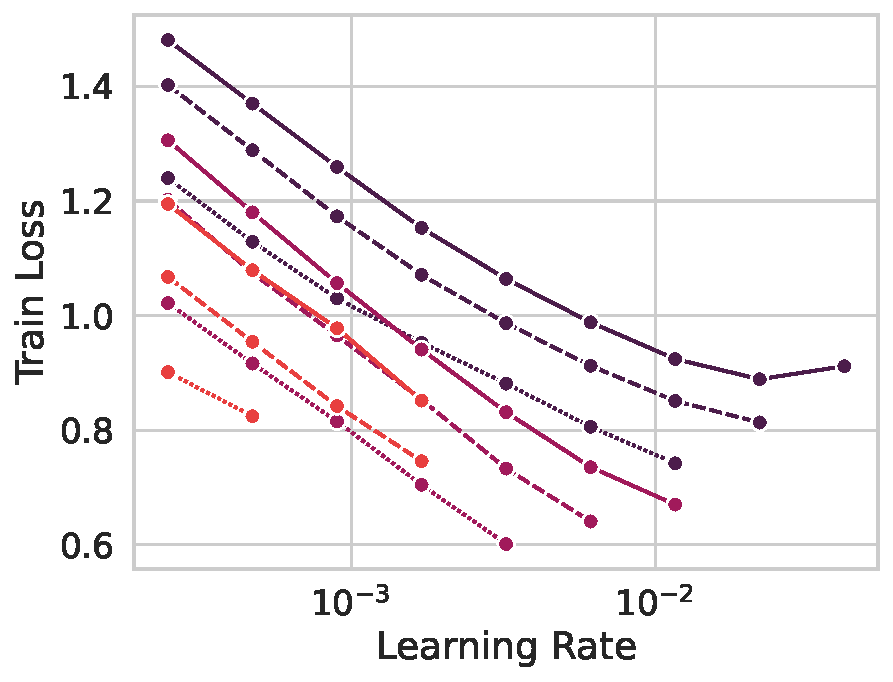
\includegraphics[width=0.425\linewidth]{figures/conv_cifar10_sp_small.pdf}}
    % 
    %\subfigure[ResNet, $\mu$P]{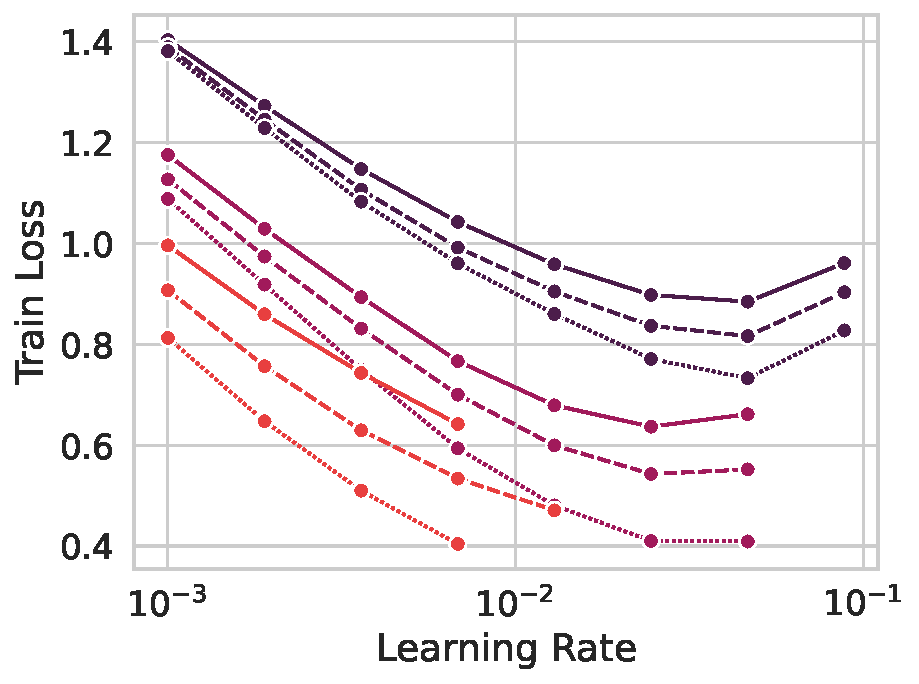
\includegraphics[width=0.44\linewidth]{figures/conv_cifar10_no_res_scaling_small.pdf}}
    % 
    %\subfigure[This work: $\frac{1}{\sqrt L}$-ResNet + $\mu$P]{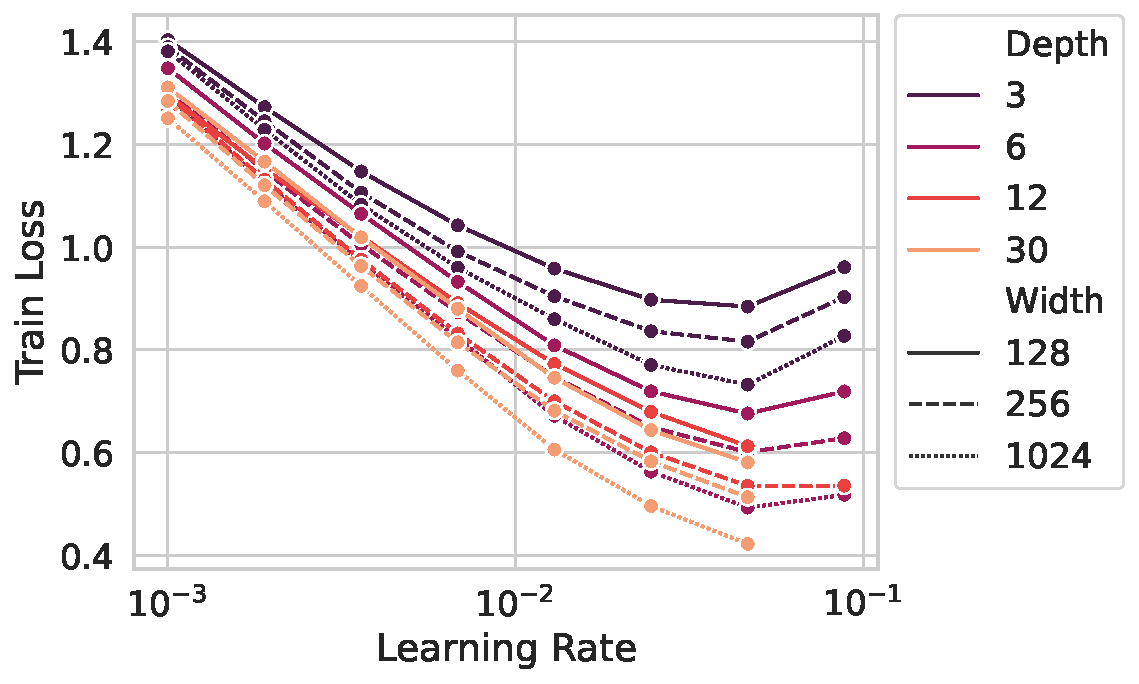
\includegraphics[width=0.545\linewidth]{figures/conv_cifar10_res_scaling_small.pdf}}
    \subfigure[ResNet, $\mu$P]{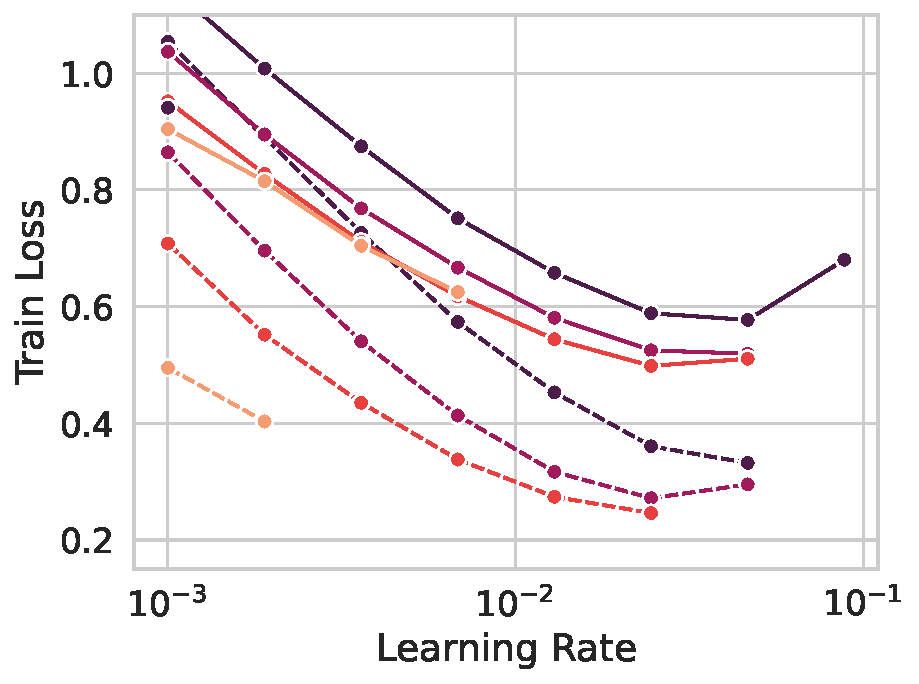
\includegraphics[width=0.44\linewidth]{figures/conv_cifar10_mup.pdf}}
    % 
    \subfigure[This work: $\frac{1}{\sqrt L}$-ResNet + $\mu$P]{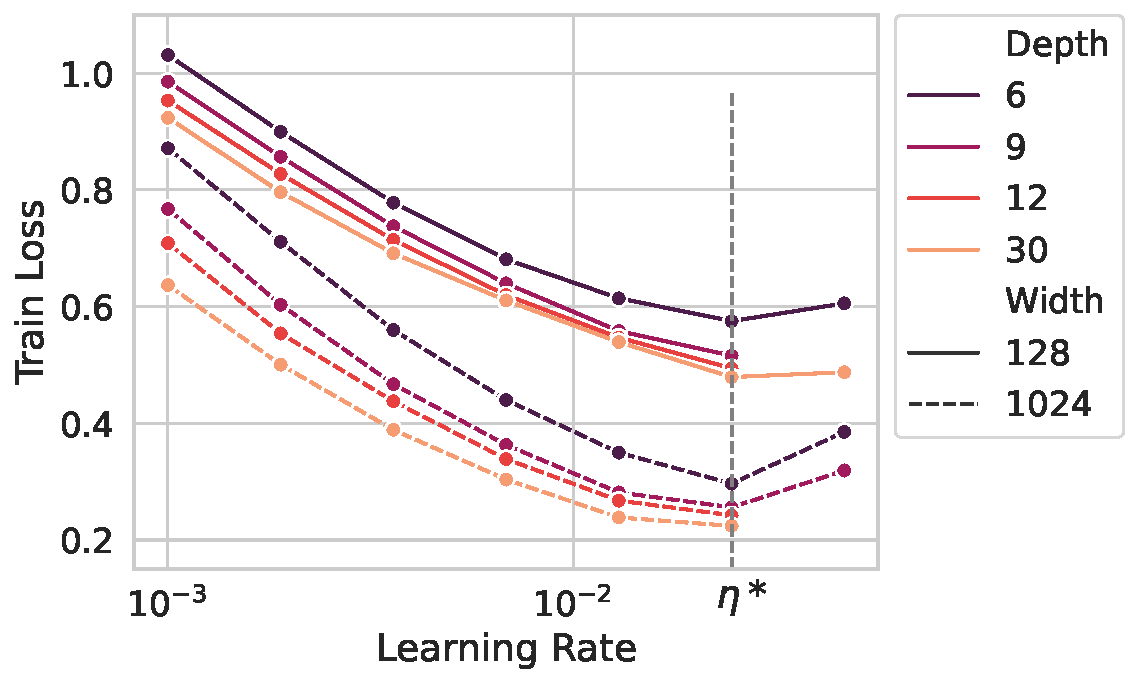
\includegraphics[width=0.545\linewidth]{figures/conv_cifar10_res_scaling_depth_beta_3.pdf}}
    \caption{The optimal learning rate $\eta^*$ transfers across both depth and width in our proposed parameterization but not in $\mu$P or standard parameterization (Fig.~\ref{fig:lr-transfer-sp}). Loss is plotted after $20$ epochs on CIFAR-10. %Points not shown represent divergences. 
    {\it All the missing datapoints indicate that the corresponding run diverged.} }% Loss is plotted after $20$ epochs on CIFAR-10. %Points not shown represent divergences. 
    %{\it All the missing datapoints indicate that the corresponding run diverged.} In particular, all depth $30$ runs diverged when using $\mu$P without $1/\sqrt{\text{depth}}$ scaling.{\color{blue} Our theory predicts larger depth in $\mu P$ corresponds to an effectively higher learning rate. $\mu P$ models are therefore expected to be closer to convergence, until the effective learning rate is so high they diverge altogether.}
    
    \label{fig:lr-transfer}
\end{figure}

%\begin{enumerate}
%    \item Figures
%    \item Hyperparameter transfer is important/costly
%    \item Introduce $\mu$P (no details?), transfers over width but does not scale with depth. 
%    \item We propose a scaling that works - here's what it is 
%    \item Discuss figures a bit 
%    \item This is motivated by theory and etc (axiomatically). 
%\end{enumerate}

% \cp{need to somehow point that missing points on the figure are diverging.} 

%{\color{blue}
%The typical pipeline for training modern neural networks involves searching over optimization hyperparameters, such as learning rates and their schedules. The computation required for such hyperparameter scans grows significantly with model size. To combat this, an influential recent line of work ? on the so-called $\mu$P parameterization seeks to develop principles by which  optimal hyperparameters from small networks can be reused — or transferred — to larger networks. The $\mu$P prescription focuses on transfer from narrower to wider models, but does not always transfer across depth (see Figure ?). The main empirical contributions of this article are as follows:

% \begin{itemize}

% 	\item We show that a simple variant of the $\mu$P parameterization allows for transfer of learning rates simultaneously across depth and width in residual networks with $1/\sqrt{\text{depth}}$ scaling on the residual branches (see \S ?? for the exact parameterization). Specifically,
%  \begin{itemize}
%      \item We show that learning rates in ResNets with $\mu$P parameterization do not transfer over depth (Figure ?)
%      \item We further show that, while learning rates transfer is improved in $\mu$P ResNets with normalization layers, the transfer is still not as good as with our $1/\sqrt{\text{depth}}$ residual branches (Figure ??). 
%      \item We show transfer for learning rates, as well as other important hyperparameters such as momentum coefficient and regularization strengths, in convolutional residual networks networks both with and without normalization trained on CIFAR-10, Tiny ImagaNet, and ImageNet. See Figures ?? and \S \ref{sec:?} for details.
%      \item We show ??? that not only do learning rates but also \textit{learning rate schedules} transfer simultaneously across depth and width in residual networks with $1/\sqrt{\text{depth}}$ scaled residual branches. 
%  \end{itemize}

% 	\item While most of our experiments concern residual convolutional networks, such as wide ResNets, we also  present preliminary evidence that our prescription leads to learning rate transfer in Vision Transformers. See Figures ??.

% \end{itemize}

% The key theoretical idea underpinning our prescription for hyperparameter transfer is that two neural networks will exhibit similar training dynamics (and hence similar optimal hyperparameters) if they are both finite size approximations to, or discretizations of, some common continuous model. Our main theoretical contributions are therefore:

% \begin{itemize}

% \item We show the infinite width and depth limit of a residual network with $1/\sqrt{\text{depth}}$ residual branch scaling and $\mu$P initialization can be characterized by a dynamical mean field theory (DMFT) ?? where the layer index takes on a continuous ``layer time." In general, the network's internal features evolve to fit the data. We show that a lazy limit of the DMFT dynamics, where features are frozen, can also be analyzed by solving the ODE at initialization. See \S ? and Theorems ??.

% \item We provide exact solutions of the DMFT dynamics in the rich (i.e. non-kernel) regime for a simple deep linear network. See \S ??.
% \end{itemize}
% }



%\cp{refer to the SP figure in the caption}
%Larger models have been consistently yielding better performance in many areas of deep learning recently, resulting in practitioners pursuing models with more than hundreds of billions of parameters \citep{kaplan2020scaling, hoffmann2022training, zhai2022scaling, klug2023scaling, openai2023gpt4}. 
% 
%However, to fine tune these algorithms to perform at their best, it is often necessary to conduct a trial-and-error style search over a grid of hyperparameters, in order to find the optimal choices. 
% 
%With the scale of the models at their incredible sizes today, this tuning procedure has become prohibitively expensive, thus becoming a bottleneck in a finite computing budget. 


Increasing the number of parameters in a neural network has led to consistent and often dramatic improvements in model quality \citep{kaplan2020scaling, hoffmann2022training, zhai2022scaling, klug2023scaling, openai2023gpt4}. To realize these gains, however, it is typically necessary to conduct by trial-and-error a grid search for optimal choices of hyperparameters, such as learning rates. Doing so directly in SOTA models, which may have hundreds of billions \citep{brown2020language} or even trillions of parameters \citep{fedus2022switch}, often incurs prohibitive computational costs.

%
%Ideally, one would like to perform hyperparameter tuning using a proxy of smaller networks, and then \emph{transfer} the optimal parameters to a larger scale setting using a principled parameterization of the network. 
% 
%This way, the best search results will extend to the largest network that their computing budget allows for. \lorenzo{TODO: add one or two references in this paragraph (e.g. scaling laws?) , Blake: I just added some, add more if I missed anything} 
%

%
To combat this, an influential recent line of work by \cite{yang2021tensor} proposed the so-called $\mu$P parameterization, which seeks to develop principles by which optimal hyperparameters from small networks can be reused — or \emph{transferred} — to larger networks \citep{yang2021tuning}. 
% 
The $\mu$P prescription focuses on transfer from narrower to wider models, but does not always transfer across depth (see Figure \ref{fig:lr-transfer}(a)).
%Towards this goal, \cite{yang2021tuning} devised the Maximal Update ($\mu$P) Parameterization for initializing a neural network that scales parameters such as learning rate, momentum and weight decay with respect to the width of the network, and showed that the optimal hyperparameters found using small networks transfer as the network width is increased\cp{cite, the first three sentences need some work. Discuss.}.
%
%A number of studies have since proposed schemes to tune hyperparameters using a proxy of smaller networks, with the hope that the best search results will extend to the largest network that their computing budget allows for. 
% 
%However, these optimal hyperparameters do not transfer to the desired larger depth networks (see Figure \ref{fig:lr-transfer}(b)). %\cp{add refs}\lorenzo{The thing is, I believe it is one of our contributions to show that muP does not transfer with depth for standard MLPs and ResNets. Not sure there is much out there. I'll look around :) }
%
%The reason is that crucial to a successful hyperparameter transfer is the existence of a well-defined infinite-limit with respect to the scaling quantities, such as the width and depth of the network. %\lorenzo{I think it's important to say that the model in Figure 1b does not have a well-defined depth limit, hence we should not expect the transfer to happen with respect to depth. This can be said in a number of different ways, maybe the simplest is: "and the ResNet model in Figure 1B does not admit a depth limit"}
% 
This leads us to pose the following problem: 
%
%The main source of difficulty arises from the fact that training dynamics of deep networks has a very complex interplay with architectural choices, such as the width and depth of the network. 
% 
%While existing work has an increasing grasp on the effect of width, depth scaling remains challenging to analyze. \lorenzo{We are repeating the same concept as above here.}
% 
%Without a careful parameterization, architectures such as MLPs and ResNets do not possess a non-degenerate infinite depth limit \citep{schoenholz2016deep, li2022neural}, hence the hyperparameters do not transfer as the architecture scales.
%
%For instance, one notable pathology with large depth is the degeneracy of correlation --- as the depth of a nonlinear network increases, the hidden layer correlations can often converge to a fixed point. 
% 
%The unstable forward pass results in unstable gradients and training dynamics, leading to an undesirable \emph{scaling limit}. 
%The unstable forward pass results in unstable gradients and training dynamics, but the core issue is the network parameterization leads to an undesirable \emph{scaling limit}. 
% 
%In particular, the training dynamics are \emph{inconsistent} in relation to the depth and width scaling.
%\cp{let's discuss this in person, I don't follow the argument here.} 
% 
% Therefore, the main problem of interest can be summarized as follows. 

%\textbf{Question: 
%\textit{Can we transfer hyperparameters across depths as well as widths?}}

\textbf{Question: 
\textit{Can we transfer hyperparameters simultaneously across depth and width?}}
% 
%\lorenzo{Not crucial, but should we mention feature learning as well? I wonder if in the current it might be misunderstood, in the sense that there are already well-defined depth-limits at initialization. CP: agreed, and added}

In this work, we provide an affirmative answer for a particular flexible class of residual architectures (including ResNets and transformers) with residual branches scaled like $1/\sqrt{\text{depth}}$ (see \Eqref{eq:res-model} and Table \ref{tab:parameterizations} for the exact parameterization). 
% 
%An example of learning rate transfer across depths (and widths) in our parameterization is provided in Figure \ref{fig:lr-transfer}(c).
% 
%Other hyperparameters that exhibits the transfer property include momentum, weight decay, and feature learning rate (see Figure \ref{fig:other_hyperparams_transfer}). 
% 
%Furthermore, learning rate transfer continues to hold in the presence of batch and LayerNormalization layers (see Figure \ref{fig:lr-transfer-norm-layers}). 
% 
More specifically, our empirical contributions can be summarized as follows: 
% 
\begin{itemize}
\setlength\itemsep{0em}
    \item We show that a simple variant of the $\mu$P parameterization allows for transfer of learning rates simultaneously across depth and width in residual networks with $1/\sqrt{\text{depth}}$ scaling on the residual branches (see \Eqref{eq:res-model} and Figure \ref{fig:lr-transfer}(b)). Moreover, we observe transfer not only for training with a fixed learning rate, but also with complex learning rate schedules (Figure \ref{fig:lr-transfer-vit}(a-d)).
     % 
    \item \looseness=-1 
     % 
      We show that the lack of learning rate transfer across depth in $\mu$P ResNets can be partly overcome by adding normalization layers (Figure \ref{fig:lr-transfer-norm-layers-bn}). However, we find on CIFAR-10, Tiny ImageNet, ImageNet, that the transfer can be significantly improved with our $1/\sqrt{\text{depth}}$ residual branches (Figures \ref{fig:lr-transfer-vit} and \ref{fig:ImageNet_expts}). 
     %Learning rate transfer also holds on Tiny ImageNet and ImageNet datasets (Figures \ref{fig:lr-transfer-vit} and \ref{fig:ImageNet_expts}).
    \item While most of our experiments concern residual convolutional networks, such as wide ResNets, we also present evidence that our prescription leads to learning rate transfer in Vision Transformers (ViTs),  both with and \emph{without} normalization
    (Figure \ref{fig:lr-transfer-vit}).
    %
     \item We demonstrate transfer for learning rates, as well as other hyperparameters such as momentum coefficients and regularization strengths in convolutional residual networks (Figure \ref{fig:other_hyperparams_transfer}).
    % 
\end{itemize}


\begin{figure}[t!]
    \centering
    \subfigure[ResNet + $\mu$P, BatchNorm]{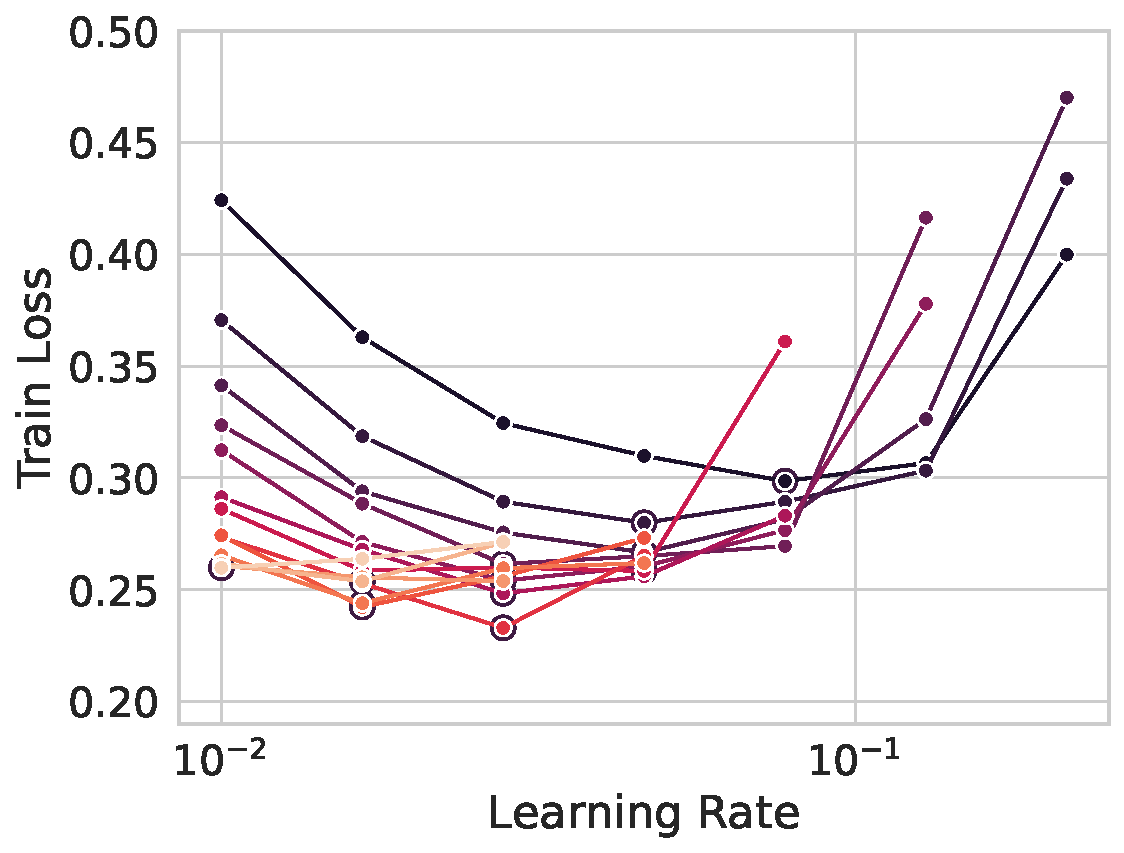
\includegraphics[width=0.43\linewidth]{figures/resnet_cifar10_bn_deep.pdf}}
    \subfigure[$\frac{1}{\sqrt L}$ ResNet + $\mu$P, BatchNorm]{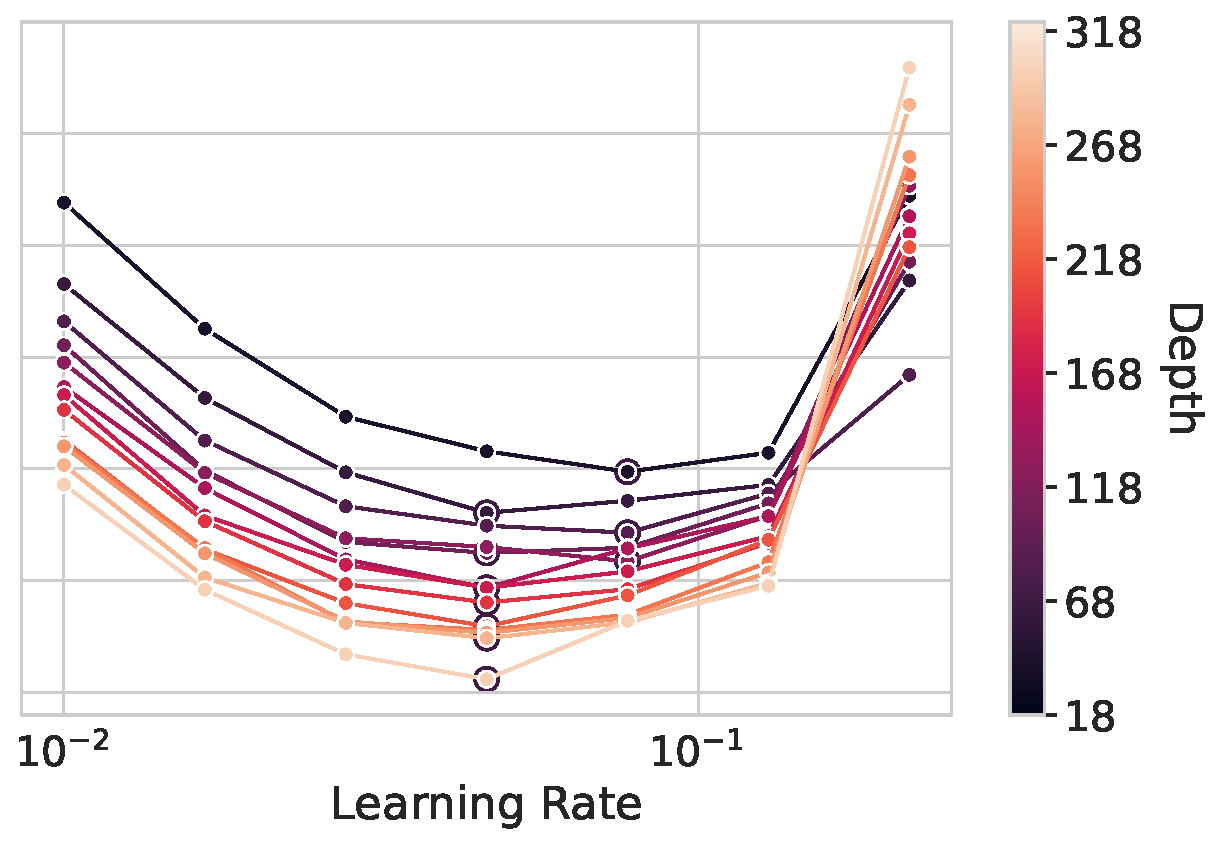
\includegraphics[width=0.466\linewidth]{figures/resnet_cifar10_res_scaling_bn_deep.pdf}}
    \caption{Effect of batch normalization on a standard Resnet18-type architecture \citep{he2016deep}. The above examples are taken after $20$ epochs on CIFAR-10. Normalization layers can slightly improve consistency and trainability across depths in standard ResNets, but consistency is much more reliable with the $1/\sqrt L$ scaling (precisely, we use $\beta_\ell = 3/\sqrt{L}$ here to increase feature learning at finite depth). Runs that exceed a target loss of 0.5 are removed from the plot for visual clarity.}
    \label{fig:lr-transfer-norm-layers-bn}
\end{figure}


%The study of neural network scaling limits started with the seminal work of Neal \citep{neal2012bayesian}, and thereafter a rich literature has formed around the topic of infinite width limits. 
% 
%The majority of these analyses, however, are contained in the kernel regime, where the math is simpler, but the limit fails to provide a faithful model of neural networks in practice. 
% 
%Recent progress suggests that a core property of good performing neural networks is feature learning, and more importantly, it is also closely tied with scalings that admit hyperparameter transfer. 
% 
The reason hyperparameters can transfer is due to the existence of a scaling limit where the network predictions and internal features of the model move at a rate independent of the size of the network. 
% 
The key underlying idea is that two neural networks will exhibit similar training dynamics (and hence similar optimal hyperparameters) if they are both finite size approximations to, or discretizations of, such a consistent scaling limit. 
% 
In fact, the success of the mean field or $\mu$P scaling \citep{yang2021tensor,bordelon2022self} is precisely due to the width-independent scale of feature updates. %leading to a well-behaved infinite-width limit with feature learning. 
% 
In the same spirit, we propose our parameterization so that the rate of feature updates and prediction updates are also independent of the \textit{depth} of the network. 
% 
%This is not true in standard feedforward models, or even models in ResNet models in $\mu$P (Figure\ref{fig:lr-transfer}(b)). 
% 
%Hyperparameter transfer across finite width/depth versions of our models is a natural corollary of these scaling rules. 
% 
%Therefore, it is an unsurprising consequence that the best hyperparameters continues to perform well as we increase the width towards infinity. 
% 
% The key theoretical idea underpinning our prescription for hyperparameter transfer is that two neural networks will exhibit similar training dynamics (and hence similar optimal hyperparameters) if they are both finite size approximations to, or discretizations of, some common continuous model. 
% 
Our main theoretical contributions can be summarized as follows:
% 
\begin{itemize}

\item Extending the infinite-width limit results of \citet{bordelon2022self}, we show the infinite-width-and-depth limit of a residual network with $1/\sqrt{\text{depth}}$ residual branch scaling and $\mu$P initialization can be characterized by a dynamical mean field theory (DMFT) (Section \ref{sec:large_limit_theory}, \ref{sec:large_width_depth_limit_equations}) where the layer index takes on a continuous ``layer time." In general, the network's internal features evolve during training in this limit. 
% 
We show that a lazy limit of the DMFT dynamics, where features are frozen, can also be analyzed as a special case. See Section \ref{sec:lazy_limit} and Proposition \ref{prop:lazy_limit}. 

\item We provide exact solutions of the DMFT dynamics in the rich (i.e.~non-kernel) regime for a simple deep linear network. See Section \ref{sec:deep_linear_DMFT}.
\end{itemize}

%We justify our proposed parameterization by deriving a large width and depth scaling limit. 
% 
%Using the framework of dynamical mean field theory (DMFT), we demonstrate that these networks indeed exhibit convergence of their training dynamics and feature learning toward the limit. 
% 
%For a special case, we can derive an exactly solveable model in Section \ref{subsec:special_exactly_solveable}. 
% 
% As a consequence, the hyperparameters can also transfer across both width and depth. 

%On the other hand, while the large depth regime has seen fruitful theories at initialization, training dynamics continues to evade tractable analysis. 
% 
%As mentioned earlier, a basic requirement for any large depth scaling is to prevent the degeneracy of correlations. 
% 
%To this end, many have proposed weakening the effect of nonlinearities with a depth dependent scaling, either by linearizing the activation function, or by reducing the residual connection weighting. 
% 
% To obtain consistent dynamics and transfer across depths, we weaken the entire block of a network with skip connections, and a $1/\sqrt{L}$ weighting on the residual branch for a ResNet with $L$ branches. 
% % 
% Finite depth ResNets of this type can be viewed as a discretization of a differential equation, hence the limit is well defined. 
% % 
% More precisely, the ResNet we consider will also be equipped with the $\mu$P scaling for the output and learning rate, as otherwise the scaling will remain in the kernel regime at large width. 
% % 
% [Add conclusion/transition] 



% Deep learning training and generalization dynamics have a nontrivial dependence on architectural choices such as network width and depth. In spite of the complexity of modern deep learning systems, recent progress has been made in identifying scaling rules and parameterizations of networks that give well defined infinite width limits which preserve feature learning. Further, these limits often behave similarly to finite networks in these parameterizations. In particular, the $\mu$P scaling has been shown to exhibit consistent optimal hyperparameters (learning rate, batch size, etc) across network widths. This consistency allows one to sweep over hyperparameters in a small model, selecting the optimal hyperparameters, and then training the larger model once with the optimal hyperparameters. 

% Given the success of $\mu$P in giving consistent dynamics and hyperparameter transfer across widths, we investigate the following natural question.

% \textbf{Question: \textit{Are there parameterizations of deep neural networks that give consistent dynamics and hyperparameter transfer across depths?}}

% Though we are not certain that \textit{any} general architecture will support such consistency, our work answers in the affirmative for a class of residual networks (ResNets). 
% 
%More concretely, we summarize our novel contributions as follows: 
% 
%\begin{itemize}
%    \item We show that ResNets with $\frac{1}{\sqrt L}$ branches and $\mu$P scaling of width exhibit convergent dynamics and hyperparameter transfer on CIFAR-10 and ImageNet training over depth and width. These models can train at large depths with or \textit{without normalization layers}.
%    % 
%    \item We justify this consistency in dynamics and hyperparameter dependence by characterizing a limiting process for the network's training dynamics in the the large width and depth limit $N,L \to \infty$. 
    % 
    %\item We show this limit can be characterized by a dynamical mean field theory (DMFT) where the layer index takes on a continuous ``layer time." In general, the network's internal features evolve to fit the data. A lazy limit of the dynamics, where features are frozen, can also be analyzed by solving the ODE at initialization. We provide exact solutions in the rich (non-kernel) regime for a simple deep linear network.
    % 
    %Throughout training, the preactivations follow an SDE and the kernels follow an ODE over layer time. We provide a special exactly solveable example of this ODE for a linear network.
    %\item We demonstrate that learning dynamics in this parameterization gives a nontrivial sequential infinite width $N \to \infty$ then infinite depth $L \to \infty$ limit with training time and the scale of feature learning independent of either $N$ or $L$. 
    % 
    %\item We characterize the finite width and depth approximation errors of the limit and provide simple experiments confirming the scaling.
%\end{itemize}

The rest of the article is organized as follows. In Section \ref{sec:framework}, we define our parameterization and scaling rules. In Section \ref{sec:empirical} demonstrate our empirical results on hyperparameter transfer. 
% 
Then in Section \ref{sec:large_limit_theory}, we proceed to characterize the limiting process at infinite width and depth and the approximation error at finite $N,L$. 
% 
Next we provide a brief overview of related works in Section \ref{sec:related_works}, before concluding with a discussion of limitations and future directions in Section \ref{sec:discussion}. 
% 
%Finally in Section \ref{sec:tradeoff}, we explore depth-consistency on ImageNet and explore the tradeoff between depth and width in this parameterization on CIFAR-10. 


% \section{Hyperparameter Transfer across Depth and Width}
% \section{High Level Instructions for Parameterization Depth-Transfer}
\section{Framework for Depthwise Hyperparameter Transfer}
\label{sec:framework}

We consider the following type of residual network (and suitable architectural/optimization generalizations, see Appendix \ref{app:arch_opt_extension}) of width $N$ and depth $L$ with inputs $\x \in \mathbb{R}^D$ which are mapped to $N$-dimensional preactivations $\h^\ell \in \mathbb{R}^N$ and outputs $f(\x) \in \mathbb{R}$:
\begin{align}
\label{eq:res-model}
    f(\x) = \frac{\beta_L}{\gamma} \w^L \cdot \phi(\h^L(\x)) \ , \quad 
    \h^{\ell+1}(\x) &=  \h^{\ell}(\x) +   \beta_\ell \W^\ell \phi(\h^\ell(\x))  
    \ , \quad \h^{1}(\x) = \beta_0 \W^0 \x ,
    %\\
    %&\text{Activation shaping}: \h^{\ell+1} = \sqrt{1-\alpha^2} \h^{\ell} + \frac{\alpha}{\sqrt N} \bm W^\ell \h^\ell + \frac{1}{\sqrt{N} L} \W^\ell \phi(\h^\ell)
    %\\
    %&\text{Weight Decoupling}: \h^{\ell+1} = \sqrt{1-\alpha^2} \h^{\ell} + \frac{\alpha}{\sqrt N} \bm V^\ell \h^\ell + \frac{1}{\sqrt{N L}} \W^\ell \phi(\h^\ell)
\end{align}
where $\gamma$ is a scaling factor, $\phi(\cdot)$ the activation function, and the weights are initialized as $\W^\ell_{ij}\sim\mathcal{N}(0,\sigma_\ell^2)$ with a corresponding learning rate $\eta(t)$. See Table \ref{tab:parameterizations}.

% \begin{table}[t!]
% \centering
%  \begin{tabular}{|c|c|c|c|c|} 
%  \hline
%   & SP (PyTorch) & NTP & $\mu$P / Mean Field & $\mu$P$+1/\sqrt{L}$-Residual (Ours) \\ [0.5ex] 
%  \hline
%  \rule{0pt}{2.2\normalbaselineskip}
%  $\beta_\ell$ & $1$ & 
%  $\begin{cases}
%     N^{-1/2}, & \ell > 0 \\ 
%     D^{-1/2}, & \ell = 0
%  \end{cases}$ & 
%  $\begin{cases}
%     N^{-1/2}, & \ell > 0 \\ 
%     D^{-1/2}, & \ell = 0
%  \end{cases}$ &
%  % 
%  $\begin{cases}
%     N^{-1/2}, & \ell = L \\ 
%     (LN)^{-1/2}, & 0 < \ell < L \\ 
%     D^{-1/2}, & \ell = 1
%  \end{cases}$
%  \\ [0.5ex]
%   \hline
%   \rule{0pt}{0.9\normalbaselineskip}
%  % 
%  $\gamma$ & $1$ & $1$ & $\gamma_0 N^{1/2}$ & $\gamma_0 N^{1/2}$ \\ [0.5ex]
%  % 
%   \hline
%   \rule{0pt}{1\normalbaselineskip}
%  $\eta(t)$ & $\eta_0(t)$ & $\eta_0(t)$ & $\eta_0(t) \gamma_0^2 N$ & $\eta_0(t) \gamma_0^2 N$ \\ [0.5ex]
%   \hline
%   \rule{0pt}{1.5\normalbaselineskip}
%  % 
%  $\sigma_\ell^2$ & 
%  $\begin{cases}
%      N^{-1}, & \ell > 0 \\ 
%      D^{-1}, & \ell = 0
%  \end{cases}$ & $1$ & $1$ & $1$ \\ 
%  % 
%  [1ex] 
%  \hline
%  \end{tabular}
%  \caption{In the framework of \Eqref{eq:res-model}, different choices of coefficients leads to standard parameterization (SP, PyTorch default \citep{paszke2019pytorch}), Neural Tangent Parameterization (NTP), $\mu$P or Mean Field parameterization, and our $\mu$P$+ 1/\sqrt{L}$-residual branch scaling which transfers over width and depth. }
%  \label{tab:parameterizations}
% \end{table}


\begin{table}[t!]
\centering
 \begin{tabular}{|c|c|c|c|c|} 
 \hline
  & SP (PyTorch) & $\mu$P / Mean Field & $\mu$P$+1/\sqrt{L}$-Residual (Ours) \\ [0.5ex] 
 \hline
 \rule{0pt}{2.25\normalbaselineskip}
 Branch Scale $\beta_\ell$ & $1$ & 
 $\begin{cases}
    N^{-1/2}, & \ell > 0 \\ 
    D^{-1/2}, & \ell = 0
 \end{cases}$  &
 % 
 $\begin{cases}
    N^{-1/2}, & \ell = L \\ 
    (LN)^{-1/2}, & 0 < \ell < L \\ 
    D^{-1/2}, & \ell = 0
 \end{cases}$
 \\ [3.5ex]
  \hline
  \rule{0pt}{1.0\normalbaselineskip}
 % 
 Output Scale $\gamma$ & $1$ & $\gamma_0 N^{1/2}$ & $\gamma_0 N^{1/2}$ \\ [0.5ex]
 % 
  \hline
  \rule{0pt}{1.1\normalbaselineskip}
 LR Schedule $\eta(t)$  & $\eta_0(t)$ & $\eta_0(t) \gamma_0^2 N$ & $\eta_0(t) \gamma_0^2 N$ \\ [0.7ex]
  \hline
  \rule{0pt}{1.6\normalbaselineskip}
 % 
 Weight Variance $\sigma_\ell^2$ & 
 $\begin{cases}
     N^{-1}, & \ell > 0 \\ 
     D^{-1}, & \ell = 0
 \end{cases}$ & $1$ & $1$ \\ 
 % 
 [2ex] 
 \hline
 \end{tabular}
 \caption{In the framework of \Eqref{eq:res-model}, different choices of coefficients leads to standard parameterization (SP, PyTorch default \citep{paszke2019pytorch}), $\mu$P / Mean Field parameterization, and our $\mu$P$+ 1/\sqrt{L}$-residual branch scaling which transfers over width and depth.} 
 \label{tab:parameterizations}
\end{table}
%
Compared to what is commonly done in practical residual architectures, such as ResNets and Transformers, our parameterization uses the $\sqrt{L}$ factor proposed in \cite{hayou2021stable, fischer2023optimal}, and the coefficient $\gamma$ from $\mu$P, but do not use normalization layers (Table \ref{tab:parameterizations}). 
% 
%\footnote{The $1/\sqrt{N}$ (and $1/\sqrt{D}$) factor is an equivalent parameterization to the one used in practice, where it is usually incorporated through the variance of the weight's initialization, i.e. $\W^\ell_{ij}\sim \mathcal{N}(0, 1/N)$ for $\ell>0$, $\W^0_{ij}\sim \mathcal{N}(0, 1/D)$. ResNets and Transformers usually have normalization layers,  but this is not necessary if the $1/\sqrt L$ is included since dynamics are stable in the infinite limit $L\to\infty$.} 
% 
% 
The parameters $\bm\theta = \{ \W^0 ,...,\w^L \}$ are updated with a gradient based learning rule. For concreteness consider SGD which we use in many experiments (we also allow for gradient flow and other optimizers in Appendix \ref{app:arch_opt_extension}): 
% 
\begin{align}
    \bm\theta(t+1)= \bm\theta(t) - \eta(t) \ \mathbb{E}_{\x \sim \mathfrak B_t} \nabla_{\bm 
    \theta} \ \mathcal{L}[f(\bm\theta, \x)] ,
\end{align}
% 
where $\mathfrak B_t$ is the minibatch at iteration $t$, $\eta(t)$ is the learning rate schedule, and the loss function $\mathcal{L}$ depends on parameters through the predictions $f$ of the model. 

% \textbf{Standard Parameterization.} \cp{This paragraph looks out of place. We can move it to the end of this section}
% \fTBD{ML: I'm trying to shift the ``practical content'' to the front of the section, and the ``theory content'' to the back, so that a practitioner can just read the first half - if that makes sense?}\cp{I would agree, but the section does not read in a linear fashion. Also, who is this practitioner we are talking about :)? }
% \fTBD{ML: yes I need to continue rewriting a lot more before this makes sense to read... and practitioner as in someone who just want to read instructions so they train their own networks and tune hyperparameters - this was one of the main points we discussed in yesterday's meeting, hence the shift in the introduction as well}
% % 
% Although the standard practice, e.g. in PyTorch \citep{paszke2019pytorch}, do not use the $1/\sqrt{N}$ prefactors, it is equivalent to the neural tangent parameterization (NTP) by choosing $\gamma,\eta$ as constants. 
% 
% \cp{you haven't introduced what goes to infinity}

% \textbf{$\mu$-Parameterization.} 
% % 
% In this work, we study the richer feature learning (\emph{mean field}) parameterization $\gamma = \gamma_0 \sqrt{N}$, $\eta(t) = \eta_0(t)  \gamma_0^2 \ N$, where $\gamma_0, \eta_0(t)$ are independent of $N$. 

The choice of how $(\gamma, \eta(t))$ should be scaled as width $N$ and depth $L$ go to infinity determines the stability and feature learning properties of the network. 
% 
If $\gamma,\eta \sim \mathcal{O}(1)$\footnote{We use $\mathcal{O}(1)$ to denote a constant independent of width $N$ and depth $L$.} (\emph{kernel regime}), then the network evolution is stable under gradient descent, but the network does not learn features at infinite width \citep{jacot2018neural, lee2019wide, yang2021tensor}. 
% 
In this work, we study the richer feature learning (\emph{mean field}) parameterization $\gamma = \gamma_0 \sqrt{N}$, $\eta(t) = \eta_0(t)  \gamma_0^2 \ N$, where $\gamma_0, \eta_0(t)$ are independent of $N$. 
% 
In this regime, the scaling factor of $1/\gamma$ in the last layer enables feature learning at infinite width, and the constant $\gamma_0$ controls the rate of feature learning. 
% 
At fixed depth $L$, this mean field parameterization is capable of generating consistent feature learning dynamics across network widths $N$ \citep{yang2021tensor, bordelon2022self}. 

One contribution of this work is identifying how $\eta_0, \gamma_0$ should be scaled with depth $L$ in order to obtain a stable feature-learning large $L$ limit. We argue that after the $\frac{1}{\sqrt L}$ factors have been introduced the correct scaling is simply 
\begin{align}
   \eta = \eta_0 \gamma_0^2 N \ , \ \gamma = \gamma_0 \sqrt{N} \ , \  \eta_0 , \gamma_0 \sim \mathcal{O}(1) .
\end{align}
We show both theoretically and experimentally that this parameterization exhibits consistent learning dynamics and hyperparameter optima across large network depths $L$. To justify this choice, we will characterize the large width and depth $N,L \to \infty$ limit of this class of models. 

\section{Experimental Verification of Hyperparameter Transfer} \label{sec:empirical}

We report here a variety of experiments on hyperparameter transfer in residual networks. 
% 
We begin with a basic modification of \eqref{eq:res-model} by replacing fully connected layers with convolutional layers.
% 
Apart from the proposed $1/\sqrt{L}$ scaling, notice that this convolutional residual model is similar to widely adopted implementations of ResNets \citep{he2016deep}, with the main difference being the absence of normalization layers, and a single convolution operator per residual block (details in Appendix~\ref{app:exp-details}). We use this residual convolutional architecture in figures \ref{fig:lr-transfer}, \ref{fig:other_hyperparams_transfer}, \ref{fig:lr-transfer-sp} and \ref{fig:param_envelope}. 
% 
We also experiment with a practical ResNet (in figures \ref{fig:lr-transfer-norm-layers-bn}, \ref{fig:lr-transfer-norm-layers-ln}, \ref{fig:ImageNet_expts}), which has two convolutional layers per block, and normalization layers (see Appendix \ref{sec:resnet}). 
% 
Finally, we also perform selected experiments on Vision Transformers \citep{dosovitskiy2020image}, to demonstrate the broad applicability of our theoretical insights (Figure \ref{fig:lr-transfer-vit}). 
% 
Below we list the the main takeaways from our experiments. 



\begin{figure}[t]
    \centering
    \subfigure[$\frac{1}{\sqrt L}$ ViT + $\mu$P]{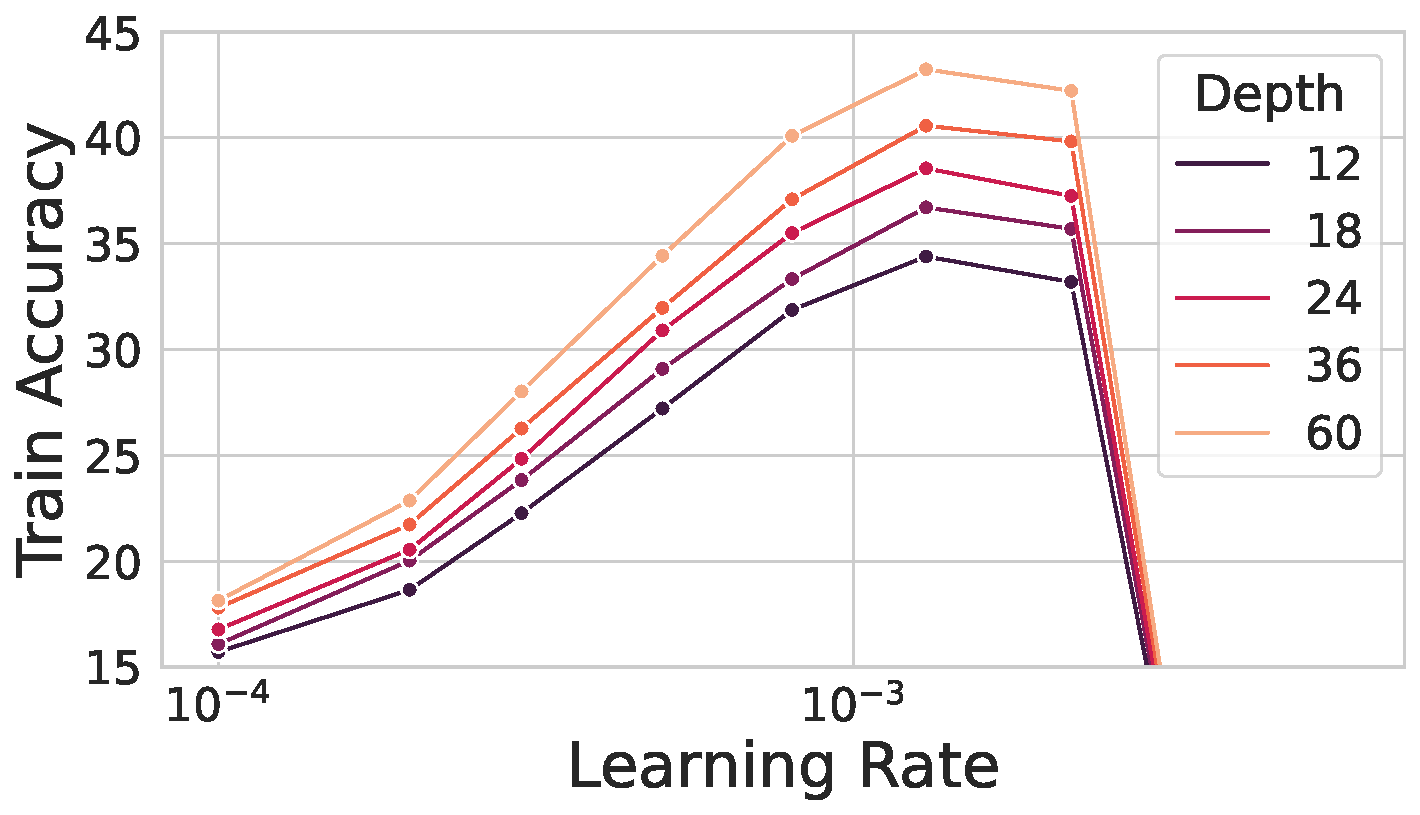
\includegraphics[width=0.32\linewidth]{figures/tiny_imgnet_vit_res_scaling_results_wu_1000.pdf}}
    \subfigure[$\frac{1}{\sqrt L}$ ViT + $\mu$P, LayerNorm]{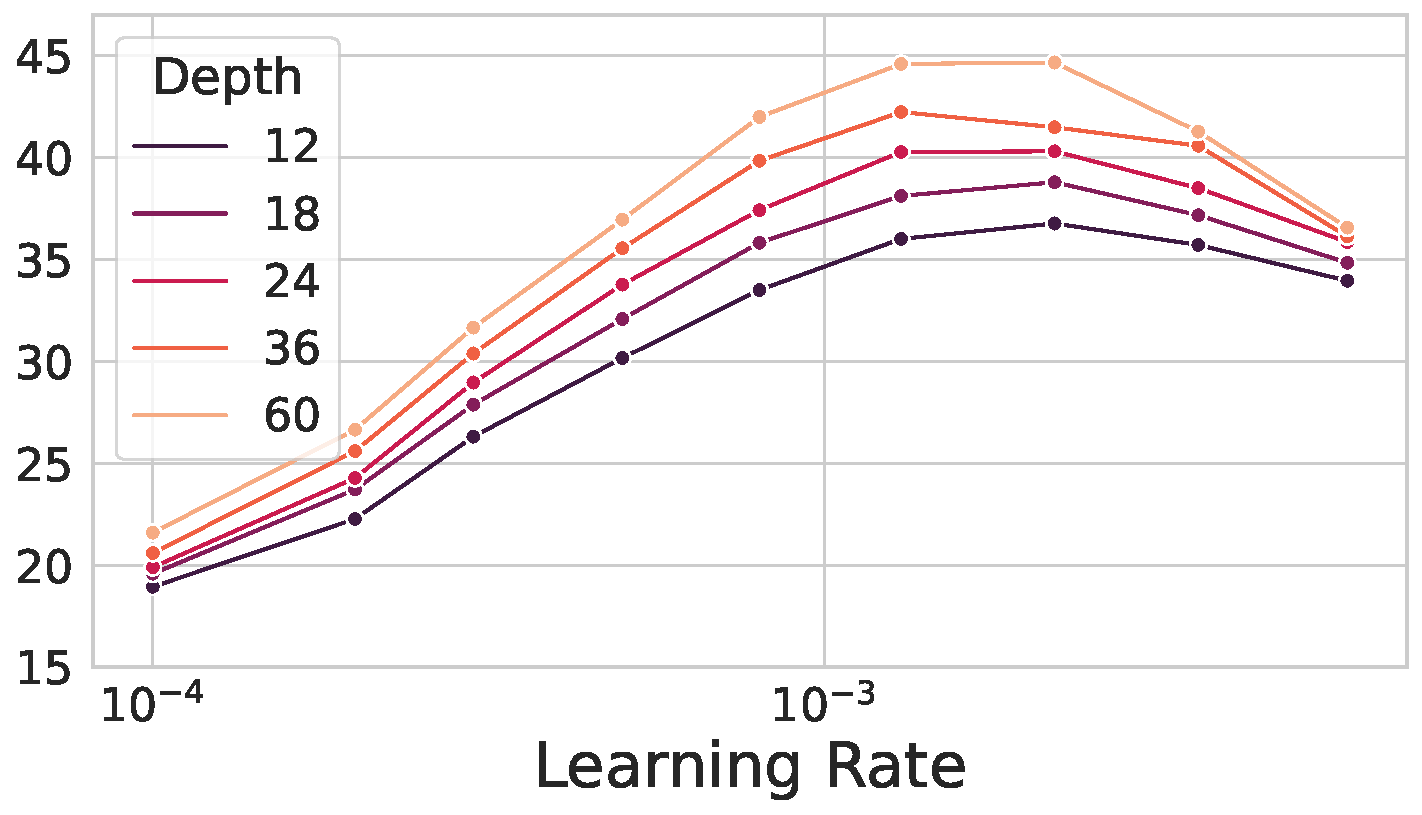
\includegraphics[width=0.32\linewidth]{figures/tiny_imgnet_vit_res_scaling_results_wu_1000_ln.pdf}}
    \subfigure[ViT + $\mu$P, LayerNorm]{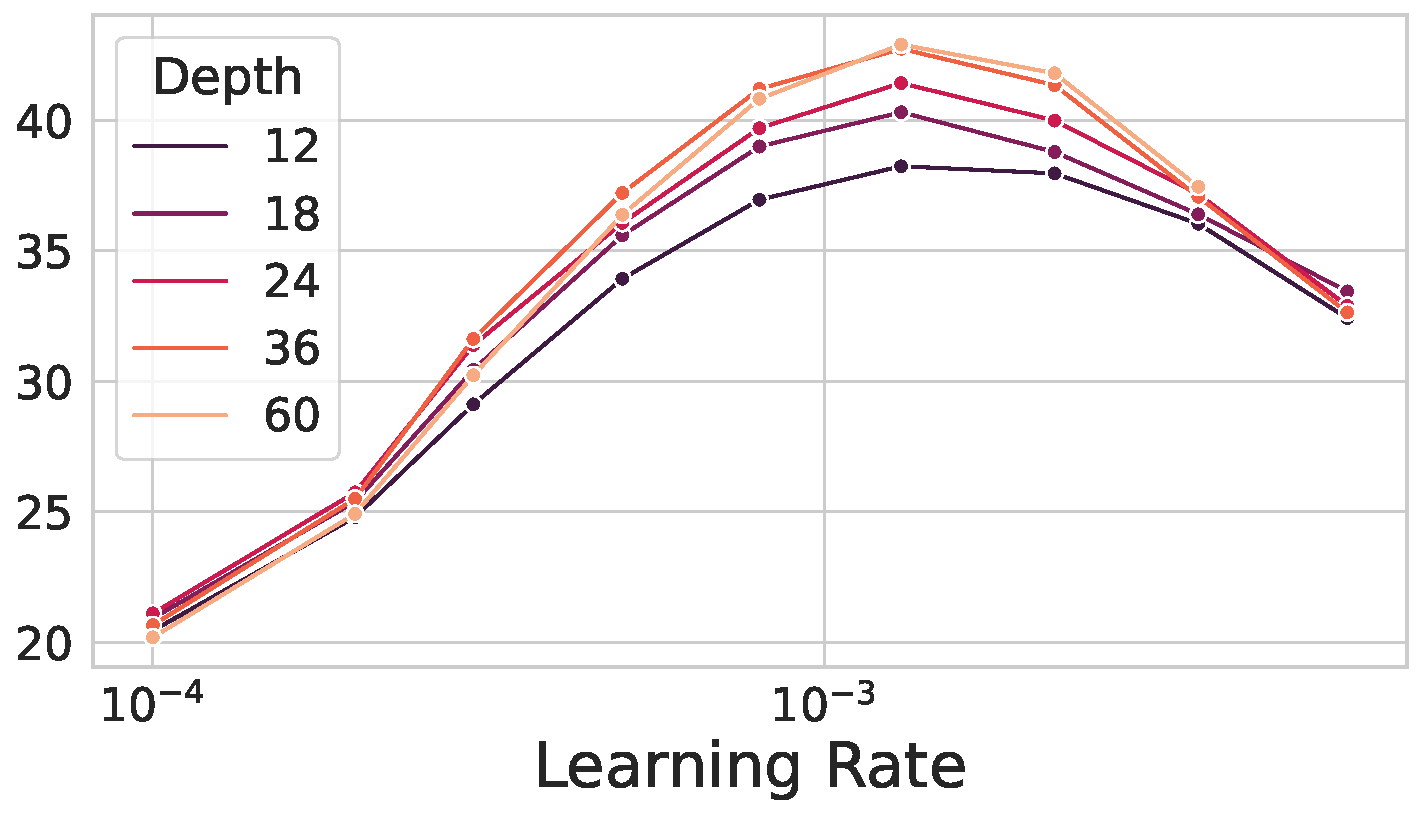
\includegraphics[width=0.32\linewidth]{figures/tiny_imgnet_vit_results_wu_1000_ln.pdf}}
    \subfigure[$\frac{1}{\sqrt L}$ ViT + $\mu$P, Cosine Annealing]{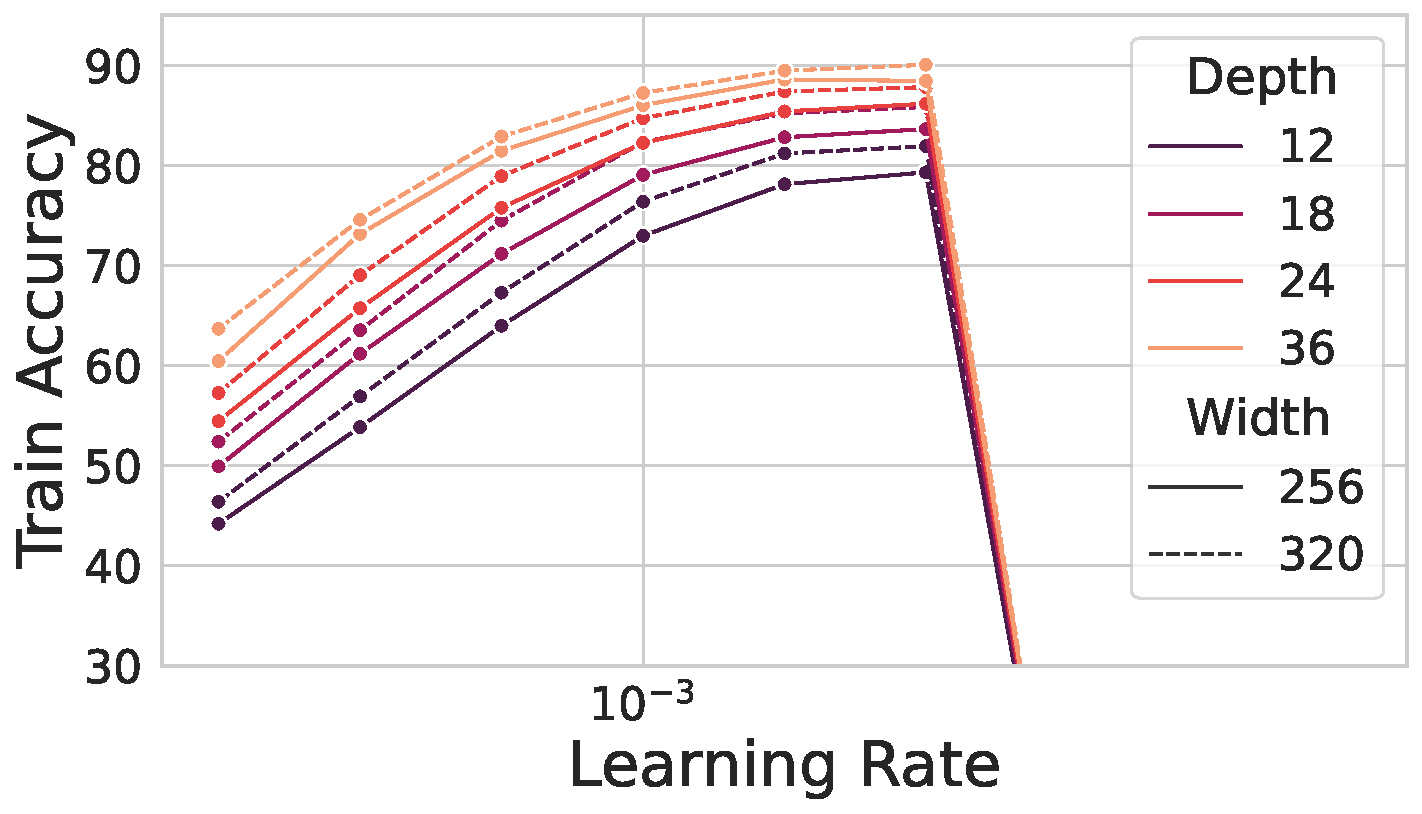
\includegraphics[width=0.33\linewidth]{figures/tiny_imgnet_vit_res_scaling_results_wu_2000_cos_schedule_100_epochs.pdf}}
    \subfigure[$\frac{1}{\sqrt L}$ ViT ImageNet Dynamics]{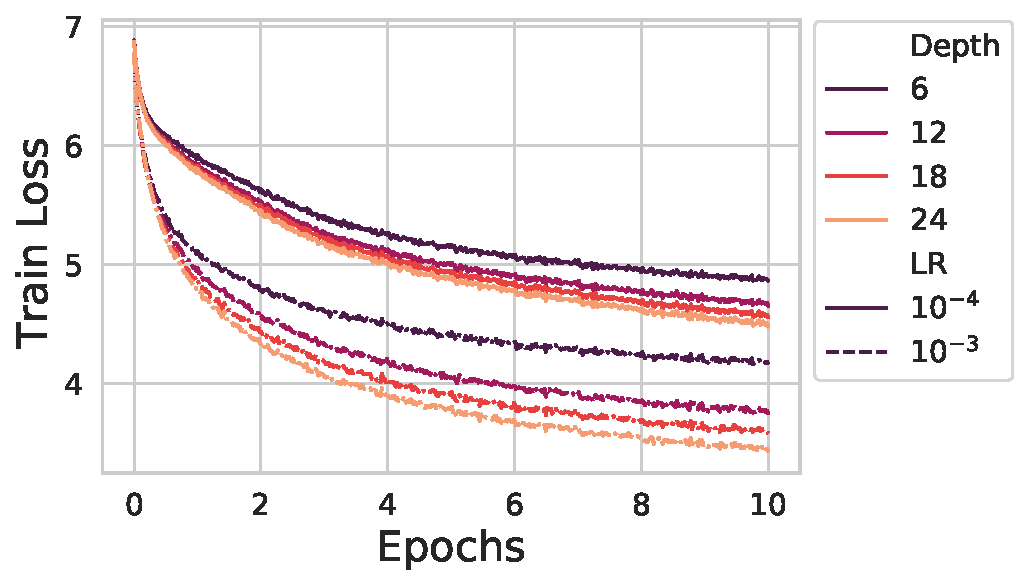
\includegraphics[width=0.34\linewidth]{figures/vit_imgnet_dynamics_deeper_better.pdf}}
    \subfigure[$\frac{1}{\sqrt L}$ ViT + $\mu$P, ImageNet ]{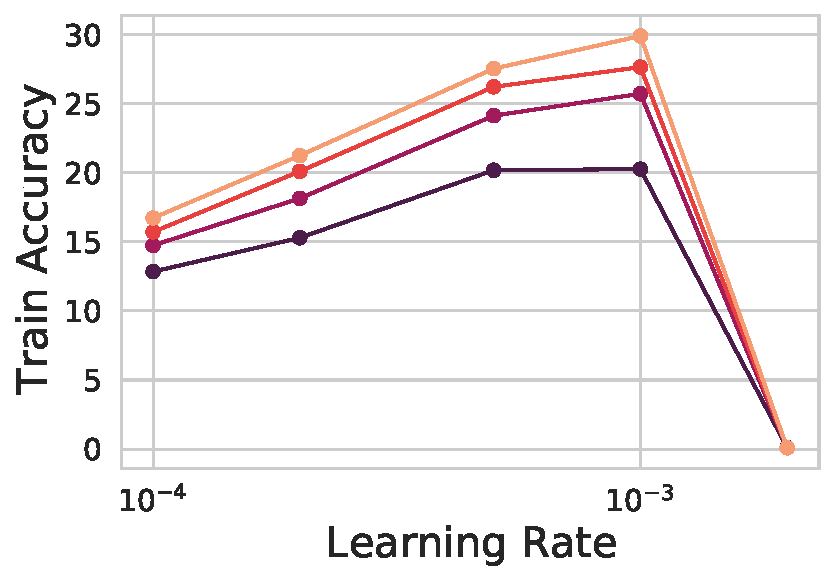
\includegraphics[width=0.3\linewidth]{figures/vit_imgnet_LR_transfer_train_acc.pdf}}
    \caption{ViTs trained with Adam also exhibit learning rate transfer, with or without LayerNorm and $1/\sqrt{L}$-scaling. The above examples are taken after 20 epochs on Tiny ImageNet for (a)-(d) and ImageNet after $10$ epochs for (e)-(f). In (a)-(c), the learning rate is linearly increased to the target in the first $1000$ steps. In (d), after $2000$ warm-up steps, the learning rate is decreased to zero with a cosine schedule in $100$ epochs.
    Notice that in addition to the transfer across all the settings, the $1/\sqrt{L}$ models show a stronger non-saturating benefit of deeper models. (e)-(f) ViTs on first few epochs of ImageNet. Also, notice that (a), (d), (e) and (f) refer to models \emph{without normalization layers}. %Here depth indicates the total number of residual layers, which is two times the number of blocks (one attention layer, one MLP layer). 
    }
    \label{fig:lr-transfer-vit}
\end{figure}
%
\textbf{$\mu$P does not Transfer at Large Depths.} While $\mu$P exhibits transfer over network widths, it does not immediately give transfer over network depths.  In Figure \ref{fig:lr-transfer}(a), we show the train loss after $20$ epochs on CIFAR-10. Notice how the network transfers over widths but not depths for $\mu$P. For completeness, in Fig.~\ref{fig:lr-transfer-sp} we  show that also SP does not transfer. 

%\lorenzo{I still think that we should incorporate intuitive explanation of why things do or do not transfer in this section and refer to other works / our own theoretical contributions. (e.g. I like how Greg Yang's paper does that). I do not want people experts in signal propagation to come and complain. In this case the non-trainability of the model comes from a bad initialization, in which the norm of preactivation explode. We should say that.}

\textbf{$1/\sqrt{L}$-scaled Residual Networks Transfer}. We repeat the same experiment, but now scale the residual branch by ${1}/{\sqrt L}$. The networks transfer over both width and depth (Figure \ref{fig:lr-transfer} (b)).

%\textcolor{red}{Figure 1: basic baselines + lr transfer across widths + depths on CIFAR }

\textbf{The Role of Normalization Layers}. Normalization layers, such as LayerNorm and BatchNorm, are commonly used instead of the $1/\sqrt{L}$-scaling in residual architectures. In Fig.~\ref{fig:lr-transfer-norm-layers-bn}, we repeat the learning rate transfer experiment with BatchNorm placed after the convolutional layer. In Fig.~\ref{fig:lr-transfer-norm-layers-ln} we repeat the same experiment with LayerNorm. In both cases, while it is known that the presence of normalization layers certainly helps the trainability of the model at larger depth \citep{daneshmand2021batch, joudaki2023impact}, we observe that the $1/\sqrt{L}$-scaled version exhibits a more consistent transfer across both width and depth.


\textbf{Empirical Verification on Vision Transformers with Adam.}
Despite our theory being primarily on (S)GD-based training, we empirically test whether the transfer results can be extended to Vision Transformers (ViTs) trained with $\mu$P-parameterized Adam optimizer \citep{yang2021tuning}. In particular, we consider Pre-LN Transformers \citep{xiong2020layer}, and adapt it to our setting by scaling all the residual branches by $1/\sqrt{L}$ (as in \cite{noci2022signal}), and make the architecture compatible with the $\mu$P framework of \cite{yang2021tuning} (see Appendix~\ref{sec:vit} for details). We test the variants both with and without LayerNorm. Results for 20 epochs training with the Tiny ImageNet dataset are shown in Fig.~\ref{fig:lr-transfer-vit} (a-c), where we also see a good transfer across all the settings. The observation of a good transfer with depth for Pre-LN Transformers was empirically observed for translation tasks in \cite{yang2021tuning}. Here, we additionally notice that while the performance benefits of Pre-LN Transformers saturates at large depth, the models with $1/\sqrt{L}$-scaling exhibits a more consistent improvement with depth. Finally, in Fig.~\ref{fig:lr-transfer-vit}(e-f) we successfully test scaling the learning rate transfer experiment of $1/\sqrt{L}$-scaled ViTs (without LayerNorm) to ImageNet (see Appendix \ref{app:more-exp} for ImageNet experiments with ResNets).

\textbf{Other Hyperparameters and Learning Rate Schedules also Transfer}.  Given the standard practice of using learning rate schedulers in optimizing Transformers \citep{dosovitskiy2020image, touvron2302llama}, we show that linear warm-up (Fig~\ref{fig:lr-transfer-vit}(a-c)), optionally followed by a cosine decay (Fig~\ref{fig:lr-transfer-vit}(d)) also transfer consistently. Finally, in Figure \ref{fig:other_hyperparams_transfer}, we plot the learning dynamics for momentum, weight decay, and the feature learning rate $\gamma_0$, which interpolates between the kernel and feature learning regimes \citep{bordelon2022self}. Despite the usual correct transfer, we highlight the \emph{consistency} of the dynamics, in the sense that learning curves with the same hyperparameter but different depths are remarkably similar, especially at the beginning of training.





\begin{figure}[t]
    \centering
    \subfigure[Momentum]{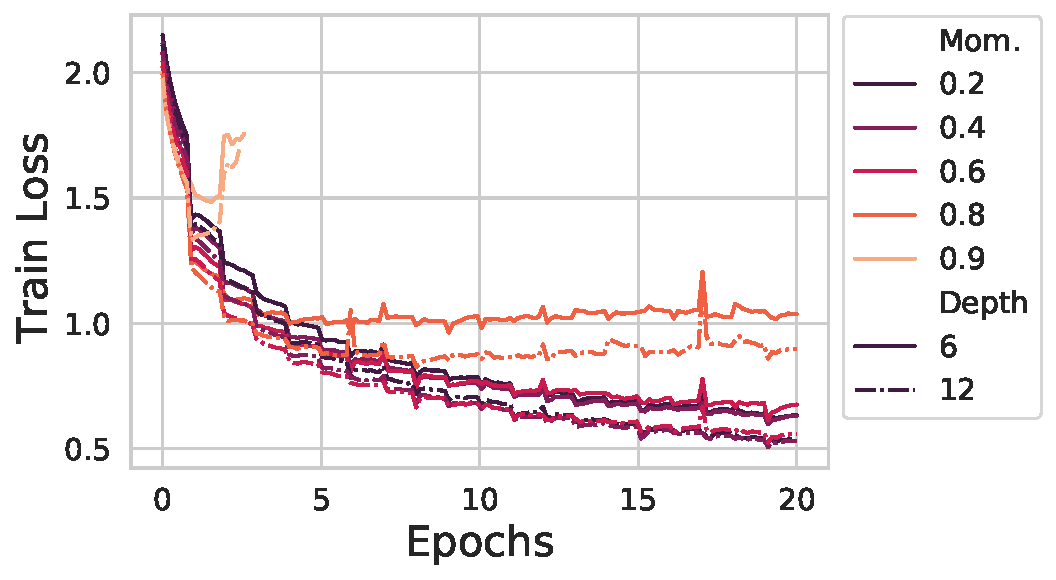
\includegraphics[width=0.475\linewidth]{figures/momentum_transfer_dynamics.pdf}}
    %\subfigure[Weight Decay]{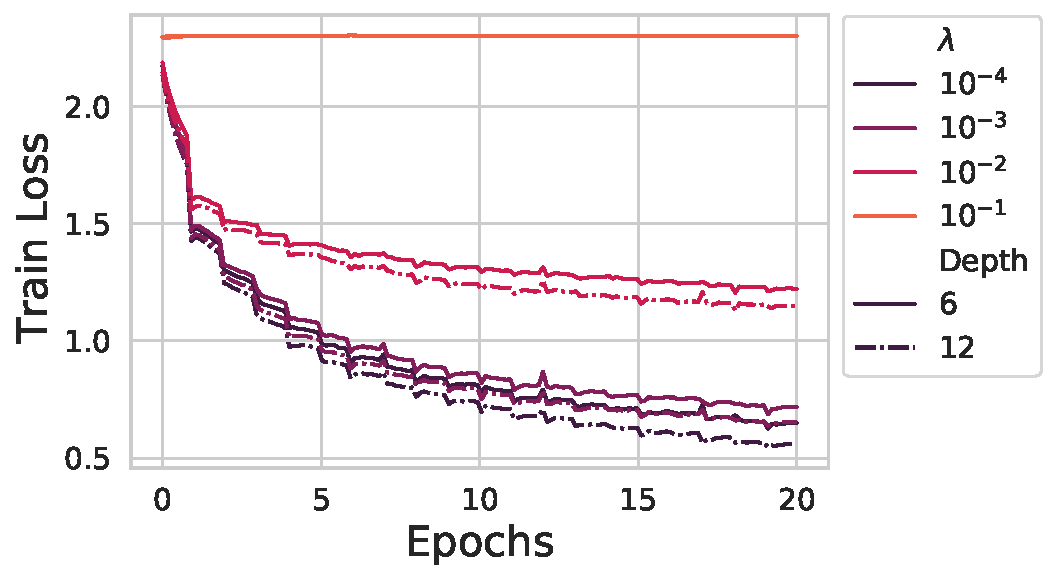
\includegraphics[width=0.335\linewidth]{figures/weight_decay_transfer_dynamics.pdf}}
    \subfigure[Feature Learning Rate $\gamma_0$]{{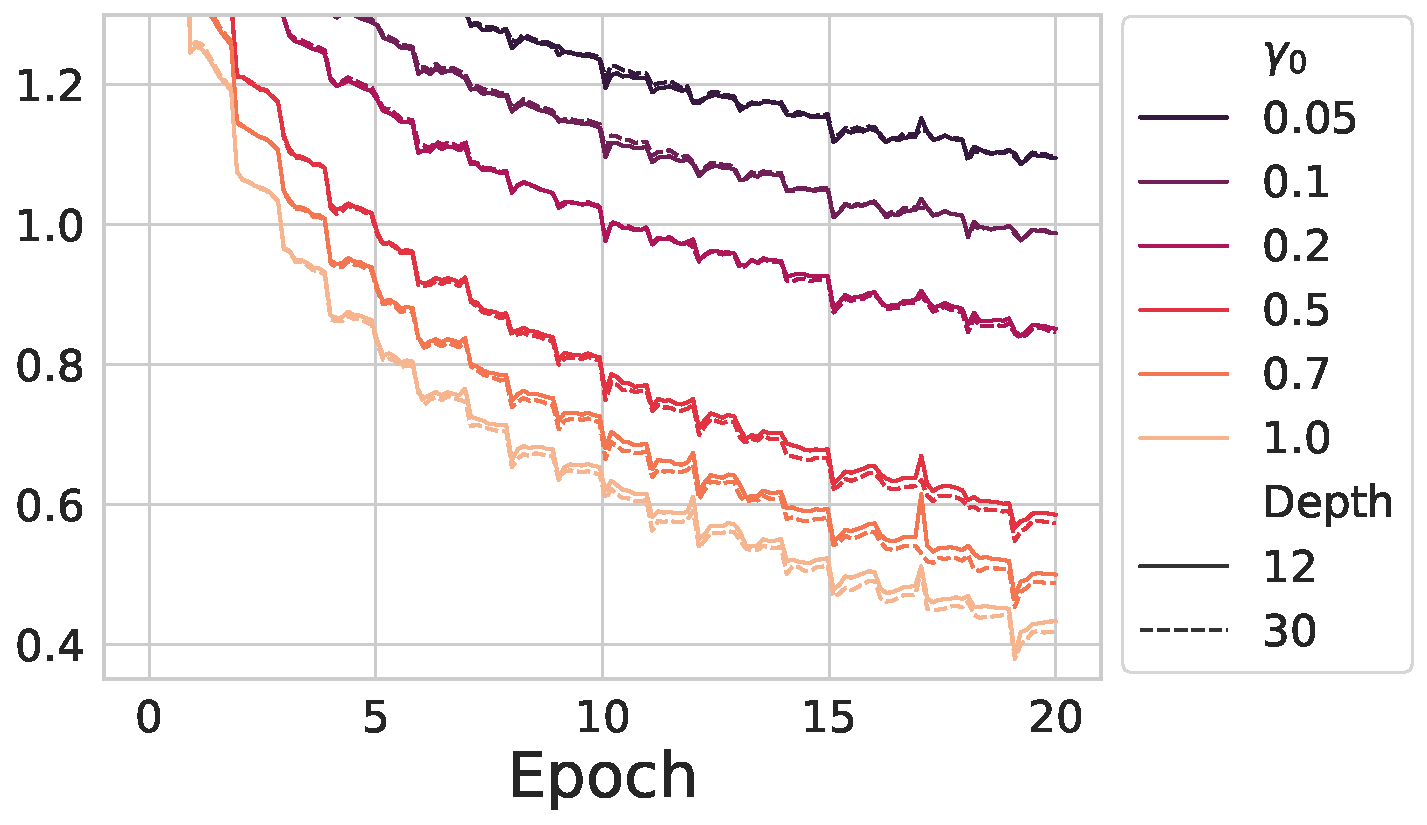
\includegraphics[width=0.45\linewidth]{figures/conv_cifar10_res_scaling_gamma_zero_sweep.pdf}}} 
    \caption{Other hyperparameters also transfer. This example shows training dynamics during the first $20$ epochs on CIFAR-10 (architecture details in Appendix \ref{app:exp-details}). The dynamics at two different depths are provided for (a) momentum (b) feature learning rate $\gamma_0$.  }
    \label{fig:other_hyperparams_transfer}
\end{figure}


\section{Convergence to the Large Width and Depth Limit}\label{sec:large_limit_theory}

We argued that width/depth-invariant feature and prediction updates are crucial for hyperparameter transfer. To formalize this, let $f_{N,L}(t)$ be the network output after $t$ steps of optimization, where we explicitly write the dependence on width $N$ and depth $L$. For hyperparameter transfer we want $f_{N,L}(t)$ to be close to $f_{N',L'}(t)$. One strategy to achieve this is to adopt a parameterization which makes finite networks as close as possible to a limit $f_{\infty, \infty}(t)$. Following this line of thought, we desire that a parameterization:
\begin{enumerate}
    \item Have a well-defined large depth and width limit, i.e. $\lim_{N,L \to \infty} f_{N,L}(t)$. %\lorenzo{I think we should not make it more formal than this (e.g. talk about Cauchy sequences, continuous functions, etc..). Also, should we say $\forall t$?} 
    \item Have internal features / kernels evolve asymptotically \emph{independent of width $N$ or depth $L$}.  
    \item Have minimal finite size approximation error. 
    %\item Have monotone improvement in performance as the size ($N$ or $L$) increases. 
\end{enumerate}
%\bb{Is this enough? Suppose I define a parameterization so that it is no feature learning for $N < 10^{6}$ but then $\mu$P for $N > 10^6$. This would have a well defined infinite width limit and would learn features in the limit. It would not be consistent in the way we want for $N < 10^6$. We need something about feature learning being independent of $N,L$!}
%
These desiderata\footnote{In addition, an ideal parameterization would also have the property that scaling up the width and depth of the model would monotonically improve performance, which empirically seems to hold in our parameterization.} motivated the $\frac{1}{\sqrt L}$-$\mu$P ResNet in \Eqref{eq:res-model} and Table \ref{tab:parameterizations}. The existence of the limit for the forward pass at initialization $t=0$ was shown in \cite{hayou2023width,cirone2023neural}. 
% 
Here, we study the learning dynamics in this model with $\mu$P parameterization, establish that the limit exists and show that feature updates are width and depth independent. 
% 
Further, we characterize the limit throughout training in Appendices \ref{app:dmft_derivation_finite_L}, \ref{app:large_L_dmft}, \ref{app:depth_first_then_width}.  
%To consider how closely finite networks approximate this limit, we consider the sources of approximation errors. Letting $f_{\infty,\infty} = \lim_{N , L \to \infty} f_{N,L}$ represent the logits of a model in the infinite limit, we find
%\begin{align}
%    \underbrace{||f_{N,L} - f_{\infty,\infty}||}_{\text{Total Finite Size Error}} \  \leq \ \underbrace{ ||f_{N,L} - \left<f_{N,L} \right>||  }_{\text{Finite Width Variance}} + \quad \underbrace{||\left<f_{N,L} \right> - f_{\infty,L}||}_{\text{Finite Width Mean Error}} \quad + \underbrace{||f_{\infty,L} - f_{\infty,\infty}||}_{\text{Finite Depth Error at Inf. Width}} ,
%\end{align}
%where $\left< \cdot \right>$ denotes an average over random initializations. We argue these three error terms asymptotically scale as $\sqrt{\frac{1}{N} \Sigma_\infty + \mathcal{O}(\frac{1}{NL})}$, $\mathcal{O}(N^{-1})$ and $\mathcal{O}(L^{-1})$ respectively where $\Sigma_\infty$ is a constant. See Appendix \ref{app:finite_N_fluctuation_scaling}, \ref{app:finite_N_L_error_analysis} for computation of the asymptotic scaling of these approximation errors. %\cp{We want to summarize the result of these computations here in a few sentences}.
%At fixed depth $L$, the predictor of the neural network converges to the infinite width feature learning limit at rate $||f_{N,L} - \left< f_{\infty,L} \right>||^2 \sim \frac{1}{N}\Sigma^\infty_f +  \mathcal{O}_{N,L}\left(\frac{1}{NL} \right)$ (see Appendix \ref{app:finite_N_fluctuation_scaling}, \ref{app:finite_N_L_error_analysis} and \cite{bordelon2023dynamics} for detailed computation of asymptotic finite-width variance $\Sigma_f^\infty$). \footnote{We note that this rate is specialized for the residual network with $\mathcal{O}(L^{-1/2})$ branch scaling. In the case of a vanilla MLP, random initializations deviate from the infinite width model as a function of $L/N$ which signal a failure for networks to converge to $f_{\infty,\infty}$ if $L$ is comparable to $N$.}. The error of the mean predictor scales as $||\left<f_{\infty,L} \right> - f_{\infty,L}||^2 \sim \mathcal{O}(N^{-2})$. Lastly, for infinite width models, we show that finite depth error goes as $||f_{\infty,L} - f_{\infty,\infty}||^2 \sim \mathcal{O}_{N,L}(L^{-2})$. %The first term is caused by a slow decay rate of the response functions with depth in the feature learning regime (App. \ref{app:response_fn_negligible}), while the second term is a discretization error of an underlying ODE (App. \ref{app:continuum_limit}).  
We attempt to visualize convergence to the limit in Figure \ref{fig:L_N_convergence plots} and Appendix Figure \ref{fig:app_ensemble_convergence_rate}. %Since we cannot compute the infinite width and depth predictor, we use a proxy $f_{\approx \infty,\infty}$: the ensemble averaged (over random inits) predictor of networks with $N=512$ and $L = 128$. 
See Appendix \ref{app:finite_N_fluctuation_scaling} and \ref{app:finite_N_L_error_analysis} for theoretical analysis of finite size approximation error and Figure \ref{fig:app_ensemble_convergence_rate} for additional tests of the sources of finite width/depth approximation error. 

\begin{figure}[t]
    \centering
    \subfigure[$N=512$ SGD Dynamics]{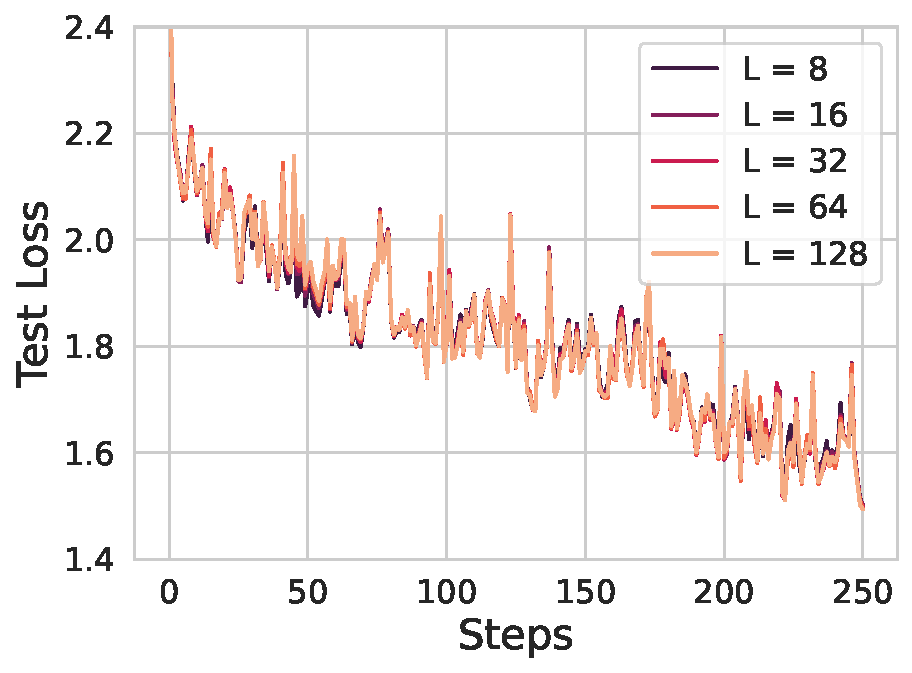
\includegraphics[width=0.375\linewidth]{figures/test_loss_consistency_early_cifar_convergence_beta_1.5.pdf}}    
    \subfigure[Convergence in $L, N$]{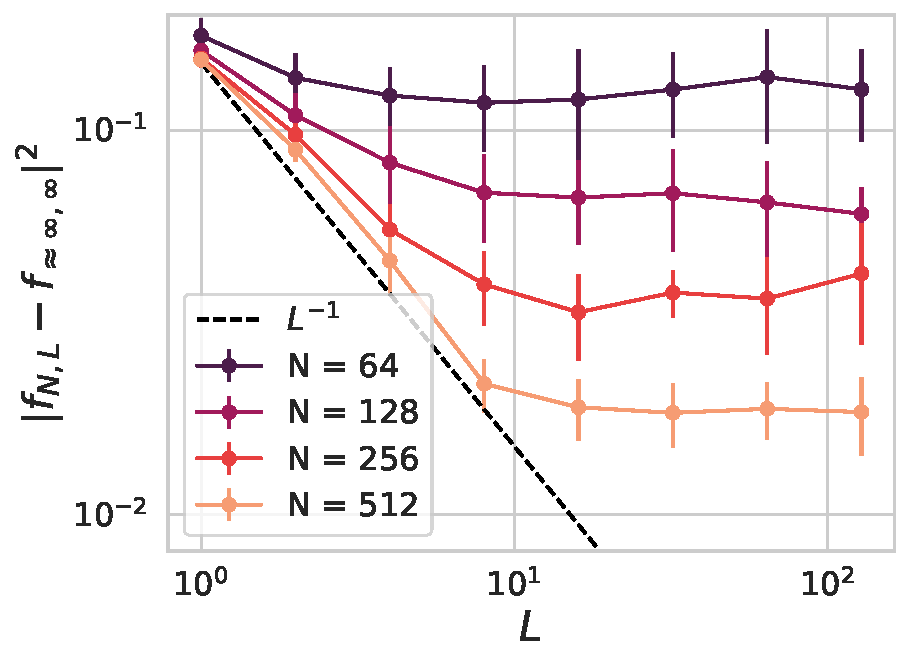
\includegraphics[width=0.375\linewidth]{figures/early_time_convergence_L_N_CIFAR_larger_batch_28_beta_1.5.pdf}}
    \caption{Approximation of the joint $N \to \infty$, $L \to \infty$ limit requires both sufficiently large $N$ and $L$. CNNs are compared after $250$ steps on CIFAR-10 with batchsize $32$ with $\gamma_0 = 1.0$. Since we cannot compute the infinite width and depth predictor, we use a proxy $f_{\approx \infty,\infty}$: the ensemble averaged (over random inits) predictor of networks with $N=512$ and $L = 128$. %Ensembled networks of of width $N=512$ and $L=128$ is used to approximate the infinite limit. 
    Error bars are standard deviation computed over $15$ random initializations. (a) SGD dynamics at large width are strikingly consistent across depths. (b) The convergence of $f_{N,L}$ to a large width and depth proxy $f_{\approx \infty, \infty}$ is bottlenecked by width $N$ for small $N$ while for large $N$, it decays like $\mathcal{O}(L^{-1})$. }
    \label{fig:L_N_convergence plots}
\end{figure}

\subsection{Primer on the DMFT in the $N \to \infty$ Limit}

To derive our theoretical results, we use a technique known as dynamical mean field theory (DMFT) \cite{bordelon2022self}. DMFT describes the dynamics of neural networks at (or near) infinite width (preserving feature learning). In this setting one tracks a set of kernel order parameters 
\begin{align}
    \Phi^{\ell}(\x,\x';t,s) = \frac{1}{N} \phi(\h^\ell(\x,t)) \cdot \phi(\h^\ell(\x',s)) \ , \quad G^{\ell}(\x,\x';t,s) = \frac{1}{N} \g^\ell(\x,t) \cdot \g^\ell(\x',s) ,
\end{align}
where $\g^\ell(\x,t) \equiv N \gamma_0 \frac{\partial f(\x,t)}{\partial \h^\ell(\x,t)}$ are the back-propagation signals. DMFT reveals the following facts about the infinite width limit:
\begin{enumerate}
    \item The dynamical kernels $\{\Phi^\ell$, $G^\ell\}$ and network outputs $f$ concentrate over random initializations of network weights throughout training. 
    \item The preactivations and gradient fields of each neuron $\{ h_i^\ell, g_i^\ell \}$ become i.i.d. random variables drawn from a \textit{single-site} (i.e. neuron marginal) density which depends on the kernels.
    \item The kernels can be computed as averages over this \textit{single-site} density.
\end{enumerate}
The last two facts provide a self-consistency interpretation: given the kernels, one can compute or sample the distribution of preactivations $\{h^\ell, g^\ell\}$. Given the density of $\{ h^\ell , g^\ell \}$, one can compute the kernels. Prior work on this limit has demonstrated that these equations can be approximately solved at finite $L$ with a Monte Carlo procedure (but with computational complexity cubic in the training iterations) \citep{bordelon2022self}. 

%Many objects concentrate at infinite width $\{ f, \Phi,G ,...\}$. \cp{the relevant objects  to the discussion below $\Phi, G, g$ should be introduced here.} The distribution of preactivation vectors factorize with a single site distribution that can be computed self-consistently. 

\subsection{The Large-Width-and-Depth Limit DMFT Equations}\label{sec:large_width_depth_limit_equations}

From the finite-$L$ DMFT equations (App. \ref{app:dmft_derivation_finite_L}), we calculate the large depth $L \to \infty$ limit, generating a continuum process over the \textit{layer time} $\tau = \frac{\ell}{L} \in [0,1]$, a concept introduced in \citet{li2022neural}. 
% 
\footnote{Alternatively, one can also take the large-$L$ limit to get a limiting \textit{distribution} over order parameters (kernels, output logits, etc) at fixed $N$, which yields the same limiting equations when $N \to \infty$ (see  App. \ref{app:depth_first_then_width}).} 

\begin{proposition}[Informal]
\label{prop:dmft_theory_expressions}
    %Consider gradient flow on data distribution $p(\x)$. The preactivations $h$ and gradient fields $g$ in the $N, L \to \infty$ limit satisfy the following stochastic dynamics 
    Consider network training dynamics of a ResNet as in \Eqref{eq:res-model} with our $\mu P$ $\frac{1}{\sqrt{L}}$ scaling and the appropriate choice of learning rate and $\gamma_0$ in the infinite width and depth limit. The preactivation $h(\tau;\x,t)$ drawn from the marginal density of neurons in a layer at layer-time $\tau$, data point $\x$ and training time $t$ obeys a stochastic integral equation
    \begin{align}
         h(\tau;\x;t) &=  h(0;\x;t) +  \int_0^\tau du(\tau';\x;t) + \eta_0 \gamma_0 \int_0^\tau d\tau' \int_0^t ds  \int d\x' C_h(\tau';\x,\x';t,s) g(\tau';\x';s)  
    %\\
    %g(\tau;\x;t) &=  g(1;\x;t) +  \int_\tau^1 dr(\tau';\x;t) \dot\phi(h(\tau';\x;t))  \nonumber
    %\\
    %&\quad+ \eta_0 \gamma_0 \int_\tau^1 d\tau' \dot\phi(h(\tau';\x;t)) \ \int_0^t ds \  \int d\x' \ %C_g(\tau';\x,\x';t,s)  g(\tau';\x';s)  .
    \end{align}
where $du(\tau;\x;t)$ is zero mean Brownian motion. The covariance of $du$ is the feature kernel $\Phi$ and the deterministic operator $C_h$ can be computed from the deterministic limiting kernels $\Phi, G$. The gradients $g(\tau)$ satisfy an analogous integral equation (See App. \ref{app:final_result_inf_width_depth} for formulas for $C_h$ and $g$). The stochastic variables $h,g$ and the kernels $\Phi, G$ satisfy a closed system of equations.
%\begin{align}
%    &C_h(\tau;\x,\x';t,s) = \Phi(\tau;\x,\x';t,s) \Delta(\x';s) p(\x') + \frac{1}{ \eta_0 \gamma_0} \left< \frac{\delta \phi(h(\tau;\x;t))}{\delta \ dr(\tau;\x';s)} \right> \nonumber
%    \\
%    &C_g(\tau;\x,\x';t,s) = G(\tau;\x,\x';t,s) \Delta(\x';s) p(\x') + \frac{1}{\eta_0 \gamma_0} \left< \frac{\delta g(\tau;\x;t)}{\delta \ du(\tau;\x';s)} \right>. 
%\end{align}
%Feature kernels $\Phi(\tau;\x,\x';t,s) = \left< \phi(h(\tau;\x;t)) \phi(h(\tau;\x';s)) \right>$ and gradient kernels $G(\tau;\x,\x';t,s) = \left< g(\tau;\x;t) g(\tau;\x';s) \right>$ are averages over the above stochastic process. 
\end{proposition}
A full proposition can be found in Appendix \ref{app:final_result_inf_width_depth}. We derive this limit in the Appendix \ref{app:large_L_dmft}, \ref{app:depth_first_then_width}. These equations are challenging to solve in the general case, as the $h$ and $g$ distributions are non-Gaussian. 
% 
Its main utility in the present work is demonstrating that there is a well-defined feature-learning infinite width and depth limit and that, in the limit, the predictions, and kernels evolve by $\mathcal{O}(1)$. 

%The NTK $K(\x,\x',t)$ at train time $t$ converges to an integral over $\tau$
%\begin{align}
%    K(\x,\x',t) = \frac{1}{L} \sum_{\ell=1}^L G^{\ell+1}(\x,\x';t,t) \Phi^{\ell}(\x,\x';t,t) \to \int_0^1 d\tau \ G(\tau; \x,\x'; t,t) \Phi(\tau; \x,\x'; t,t)
%\end{align}
%which will remain as a $\mathcal{O}(1)$ object in the large $L$ limit with error $\mathcal{O}(L^{-1})$. At infinite width, the preactivation feature in layer $\ell$, $h^\ell$ follows a stochastic process \bb{get rid of finite depth equations}
%\begin{align}\label{eq:large_depth_DMFT_h_asymptotic}
%    h^{\ell}(\x;t) &= h^{1}(\x;t) + \frac{1}{\sqrt L} \sum_{k=1}^{\ell} u^{k}(\x;t) \nonumber
%    \\
%    &+ \frac{\eta_0 \gamma_0}{L} \sum_{k=0}^{\ell-1} \int_0^t ds \ \int d\x' [ \Phi^{k}(\x,\x';t,s) \Delta(\x';s) \ p(\x') + A^{k}(\x,\x';t,s)] \ g^{k+1}(\x', s)  , 
    %\\
    %g^{\ell}(t) &\sim g^{\ell+1}(t) + \frac{1}{\sqrt L} \dot\phi(h^\ell(t)) \left[ r^\ell(t) + \frac{\eta \gamma}{\sqrt L} \int_0^t ds G^{\ell+1}(t,s) \phi(h^\ell(s))  \right]
%\end{align}
%where $u^\ell(\x,t) \sim \mathcal{GP}(0,\Phi^\ell(\x,\x';t,s))$ and $r^\ell(\x,t) \sim \mathcal{GP}(0, G^{\ell+1}(\x,\x';t,s))$ are Gaussian random sources. The response function satisfies $A^\ell(\x,\x';t,s) = \frac{\sqrt{L}}{\eta_0 \gamma_0} \left< \frac{\delta \phi(h^\ell(\x,t))}{\delta r^\ell(\x',s)} \right> \sim \mathcal{O}_L(1)$. 
% Since each of the $u^k$ terms are independent across layer index $k$, the sum with prefactor $\frac{1}{\sqrt L}$ will behave as integrated Brownian motion at large $L$. Next, the random gradient fields $g^\ell = g^{\ell+1} + \mathcal{O}(\frac{1}{\sqrt{L}})$ are \textit{correlated across all layers} due to the skip connections \footnote{Gradient fields $g^\ell$ and $g^{\ell'}$ are statistically independent for $\ell\neq \ell'$ in a vanilla feedforward (non-ResNet) model at infinite width. The long range correlations in the ResNet is what allows $\gamma_0 \sim \mathcal{O}(1)$ to give feature learning at infinite depth.}. Consequently, the final term will behave as an average over layers and converge to a $\mathcal{O}(1)$ integral. The resulting continuum limit takes the form of a stochastic process over layer time $\tau$, inputs $\x,\x'$ and training times $t,s$, \bb{introduce theorem statements}
% \begin{align}
%     &h(\tau;\x;t) =  h(0;\x;t) +  \int_0^\tau du(\tau';\x,t)  \nonumber
%     \\
%     &+ \eta_0 \gamma_0 \int_0^\tau d\tau' \ \int_0^t ds \  \int d\x' \ [ \Phi(\tau';\x,\x';t,s)\Delta(\x';s) p(\x') + A(\tau,\x,\x';t,s) ] g(\tau';\x';s)  .
% \end{align}
% The Brownian motion $du(\tau;\x;t)$ has zero mean $\left< du(\tau,\x,t) \right> = 0$ and covariance structure 
% \begin{align}
%     \left< du(\tau;\x;t) du(\tau';\x';s)  \right> = \Phi(\tau,\x,\x',t,s) \delta(\tau-\tau') d\tau
% \end{align}
% An analogous equation for $g(\tau;\x;t)$ (and also differential versions of the above) and an ODE for the feature kernels $\Phi(\tau;\x,\x';t,s), G(\tau;\x;\x';t,s)$ is provided in the Appendix \ref{app:kernel_ODEs}. We note that $\mathcal{O}(1)$ movement of the preactivation features is already achieved with $\gamma_0 \sim \mathcal{O}_L(1)$, justifying this parameterization as it gives the correct scale of feature updates at infinite depth. 

\subsection{Special Exactly Solveable Cases of the $N,L\to\infty$ DMFT equations}
\label{subsec:special_exactly_solveable}

\looseness=-1 Though the resulting DMFT equations for the kernels are intractable in the general case, we can provide analytical solutions in special cases to verify our approach. We first write down the training dynamics in the lazy limit by characterizing the neural tangent kernel (NTK) at initialization. Next, we discuss deep linear ResNets where the feature learning dynamics gives ODEs that can be closed while preserving Gaussianity of preactivations. 


\subsubsection{The Lazy Learning Limit}\label{sec:lazy_limit}

A special case of the above dynamics potentially of interest is the limit of $\gamma_0 \to 0$ where the feature kernels are frozen. In this limit the NTK $K$ is static and can be computed at initialization and used to calculate the full trajectory of the network dynamics (see Appendix \ref{app:lazy_limit}).
% 
\begin{proposition}[Informal]
\label{prop:lazy_limit}
Consider a ResNet with the $\frac{1}{\sqrt L}$-$\mu$P parameterization in the $N, L \to\infty$ limit. In the $\gamma_0 \to 0$ limit, the feature kernel $\Phi(\tau)$, gradient kernel $G(\tau)$ and NTK $K$ do not evolve during training and satisfy the following differential equations over layer time $\tau$
\begin{align}
    \partial_\tau H(\tau;\x,\x') &= \Phi(\tau;\x,\x') \ , \ \Phi(\tau;\x,\x') = \left< \phi(h) \phi(h') \right>_{h,h' \sim \mathcal{N}(0,\bm H_{\x,\x'}(\tau))} \nonumber
    \\ 
    \partial_\tau G(\tau;\x,\x') &= - G(\tau;\x,\x')\left< \dot\phi(h) \dot\phi(h') \right>_{h, h' \sim \mathcal{N}(0,\bm H_{\x,\x'}(\tau))} \nonumber 
    \\   
    \bm H_{\x,\x'}(\tau) &= \begin{bmatrix}
        H(\tau;\x,\x) & H(\tau;\x,\x')
        \\
        H(\tau;\x',\x) & H(\tau;\x',\x')
    \end{bmatrix} \  , \quad K(\x,\x') = \int_0^1 d\tau \  G(\tau,\x,\x') \Phi(\tau,\x,\x') .
\end{align}
The dynamics of the neural network outputs $f(\x,t)$ can be computed from $K(\x,\x')$.  
\end{proposition}
The forward ODE for $\Phi$ at initialization was studied by \cite{hayou2023width,cirone2023neural}. Figure \ref{fig:ReLU_at_init} shows this limiting NTK for a ReLU network. The finite depth kernels converge to the limiting large $L$ kernel (blue line in (a)) at a rate $\mathcal{O}(L^{-2})$ in square error. 

\begin{figure}[t]
    \centering
    \subfigure[ReLU NTKs at Initialization]{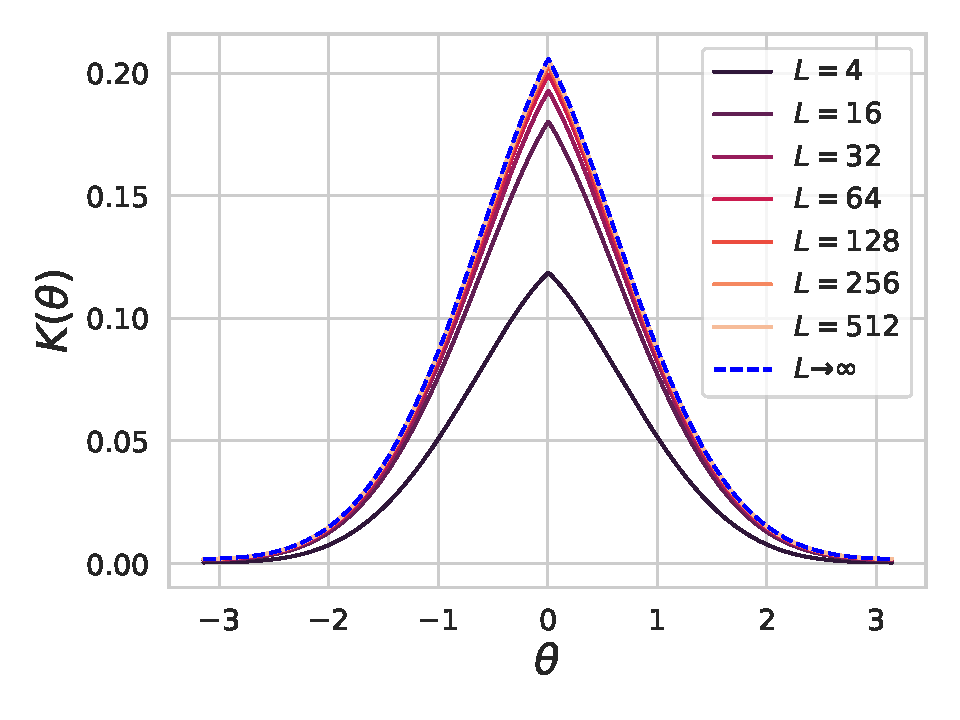
\includegraphics[width=0.38\linewidth]{figures/ntk_convergence_visual_inf_width.pdf}}
    %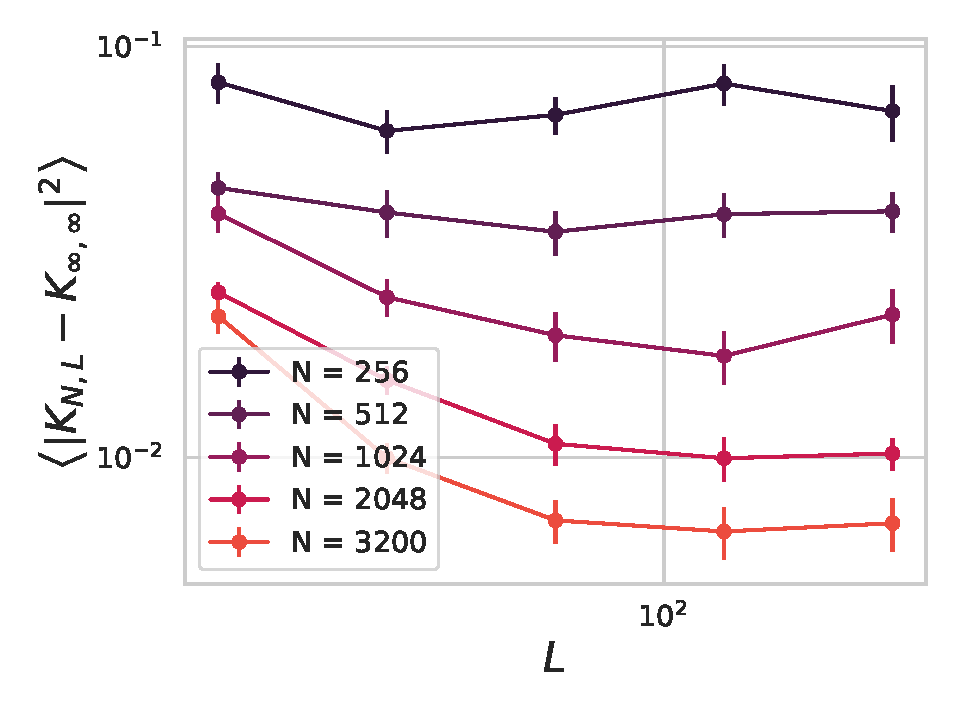
\includegraphics[width=0.32\linewidth]{figures/init_ntk_convergence_sqr_err.pdf}
    \subfigure[Initial NTK Convergence in $L$]{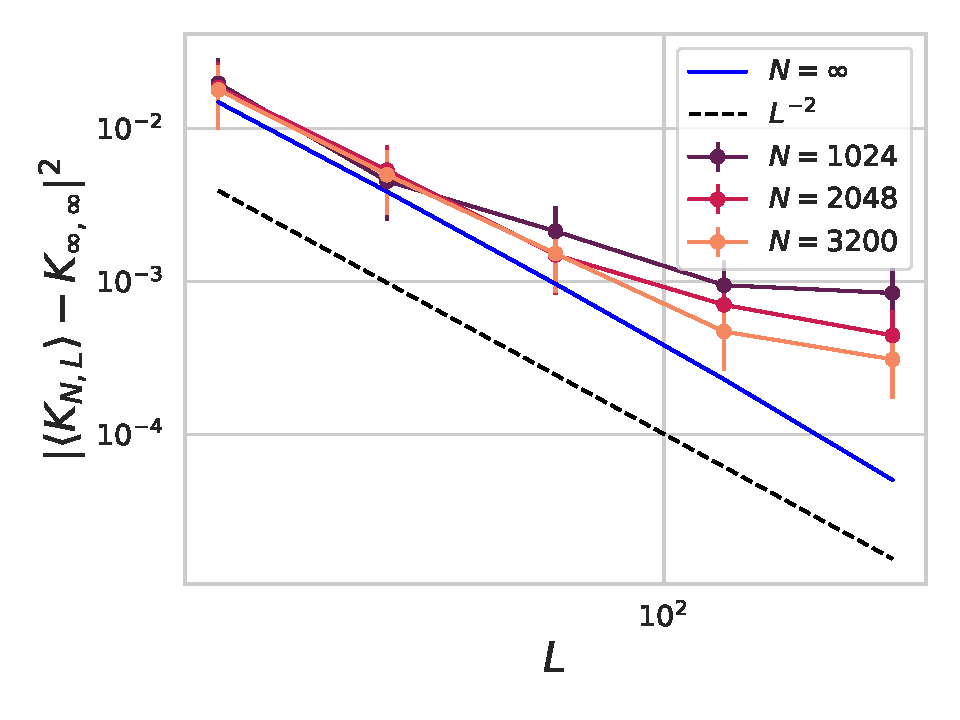
\includegraphics[width=0.38\linewidth]{figures/init_ntk_mean_convergence_sqr_err_more.pdf}}
    \caption{Convergence of the depth $L$ NTK to the limiting kernel at initialization. (a) The infinite width NTK for a ReLU residual multilayer perpectron (MLP) for two inputs $\x,\x'$ separated by angle $\theta \in [-\pi,\pi]$ over varying depth $L$. The kernel converges as $L \to \infty$. (b) The convergence rate of the initialization averaged NTK $\left< K \right>$ with network widths $N$ and network depths $L$ at initialization. For sufficiently large $N$, the \textit{initial} NTK will converge at rate $\mathcal{O}(L^{-2})$ in square error.  }
    \label{fig:ReLU_at_init}
\end{figure}

%At initialization, the kernel converges with rate $\mathcal{O}(L^{-2})$ in square error. This will also be the finite depth approximation error of the predictor function $|f_{\infty,L} - f_{\infty,\infty}|^2 \sim \mathcal{O}(L^{-2})$. 

\subsubsection{Deep Linear ResNets}\label{sec:deep_linear_DMFT}

Next we explore the dynamics of feature learning in a solveable infinite depth ResNet with linear activations. In this case, the preactivations $h$ and gradient fields $g$ remain Gaussian over the full time-course of learning, rendering the DMFT equations tractable without any need for Monte Carlo methods. As an example, in Figure \ref{fig:theory_verify} we show the kernel updates in a deep linear ResNet after a single training step on a single training example $(\x,y)$. The theoretical solution to the kernel ODE at initialization $H_0(\tau) = e^{\tau} H_0(0)$ and after one step $H_1(\tau)$ is (see Appendix \ref{app:linear_one_step} for derivation)
\begin{align}
    %&H_0(\tau) =  e^{\tau} H_0(0) \ , \ G_0(\tau) = e^{-\tau} + 1 - e^{-1} \\ \nonumber
    &H_1(\tau) = e^{\tau} H_1(0) + 2 \eta_0^2 \gamma_0^2 y^2 e^{\tau} \ \left[ \frac{1}{3} \tau^3 + \frac{1}{2}\tau^2 + (1+e^{-1})( \tau^2 e^\tau - \tau e^\tau + e^\tau - 1 ) \right] 
\end{align}
For networks with depths on the order of $\sim 100$ the infinite depth solution gives an accurate description of the profile of the kernel updates. More general equations for infinite depth linear networks are provided in Appendix \ref{app:linear_dmft_eqns}. 

\begin{figure}[t]
    \centering
    \subfigure[Kernels at initialization]{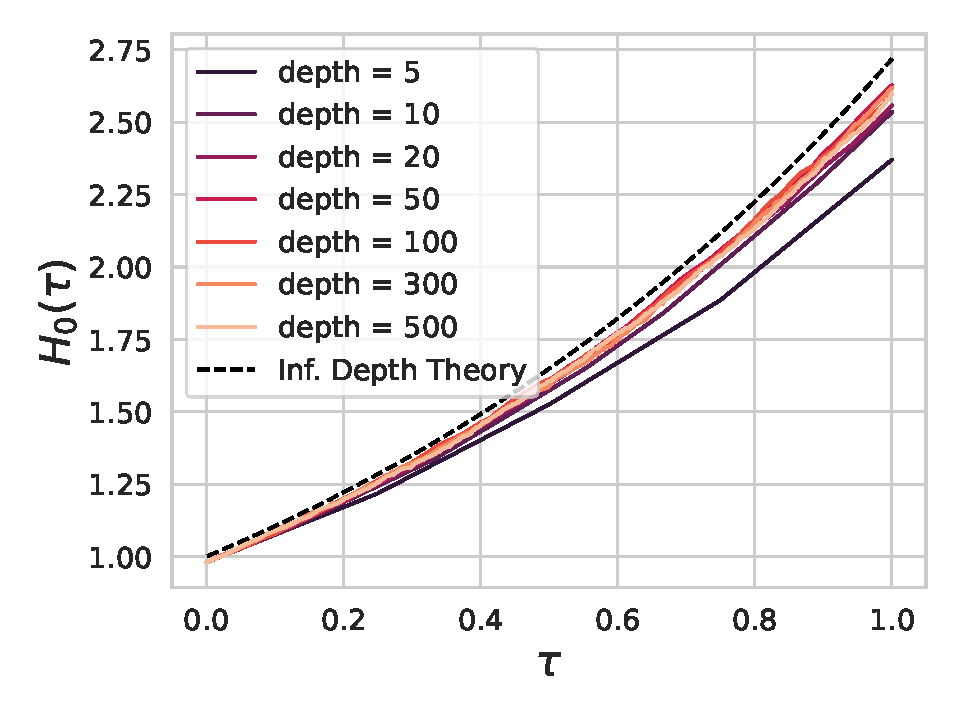
\includegraphics[width=0.38\linewidth]{figures/kernels_init_inf_theory.pdf}}
    \subfigure[Kernel Updates after 1 Step]{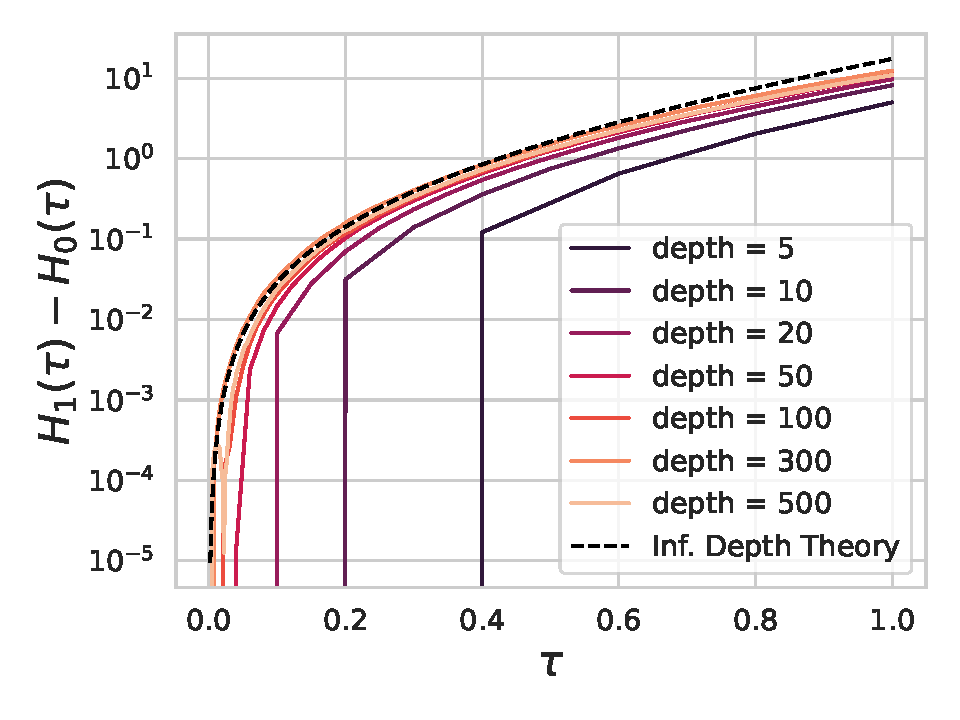
\includegraphics[width=0.38\linewidth]{figures/inf_depth_theory_linear.pdf}}
    \caption{We plot the feature kernels $H(\tau) = H^{\ell}|_{\ell = \tau L}$ in width $N = 1000$ residual linear networks before and after taking a gradient step in our parameterization. The kernel profiles at initialization $H_0(\tau)$ and the kernel changes $H_1(\tau) - H_0(\tau)$ converge for large $L$. We compare to the theoretical result expected from the $L \to \infty$ limit of the DMFT equations (dashed black).}
    \label{fig:theory_verify}
\end{figure}




%\subsection{Finite width corrections: how noisy is this limit?}

%\textcolor{red}{reason about the finite width fluctations} 

%\textcolor{red}{Show that at fixed $L, N$ the variance of the NTK and the predictor scale as $\mathcal{O}\left( \frac{1}{N L} \right)$.}

%Conjectures + expts showing correct scaling (toy models)

%\section{Depth/Width Tradeoff}
%\label{sec:tradeoff}

%Given that each finite width and depth model approximates a limiting infinite width and depth model, it is natural to wonder which kinds of approximation errors are most harmful to performance. Equivalently, how should one choose to increase width and depth to obtain the best performance? In Figure \ref{fig:param_envelope} we investigate this in CIFAR-10 with ResNet architectures. 


\section{Related Works}
\label{sec:related_works}

The $1/\sqrt{L}$-scaled residual model \citep{he2016deep} adopted in this work belongs to a rapidly expanding research domain. 
% 
This approach has several advantageous characteristics in signal propagation, in terms of dynamical isometry \citep{tarnowski2019dynamical}, as well as stable backward and forward kernels \citep{ balduzzi2017shattered, hayou2021stable, fischer2023optimal}. 
% 
As a result, this has paved the way for the development of reliable initialization methods \citep{taki2017deep, zhang2019fixup}, including Transformers without normalization layers \citep{huang2020improving, noci2022signal}. 

The study of neural network scaling limits started with MLPs in the infinite-width kernel regime \citep{jacot2018neural, neal2012bayesian, matthews2018gaussian, lee2017deep}, where the preactivations are also Gaussian with deterministic covariance. 
% 
However, the joint depth and width limit has been shown to be non-Gaussian \citep{hanin2020products, noci2021precise} and have a stochastic covariance \citep{li2021future}. 
% 
In particular, the feature covariance of particular classes of networks have a limit described by stochastic differential equations (SDEs) \citep{li2022neural,noci2023shaped}, where the layer time is the depth-to-width ratio in this case. 
% 
On the other hand, \cite{hayou2023width} study the forward signal propagation in ${1}/{\sqrt L}$-scaled ResNets at initialization, where the preactivations converge to a Gaussian distribution with a \emph{deterministic} covariance described by an ODE. 
% 
% This is a distinctive feature of this model. 
% % 
% % For MLPs the infinite-width limit converges to the well-established NTK/NNGP regime. 
% % 
% % As the randomness in the weights is taken into account by taking the limit, the covariance will stay deterministic at all depths. 
% % 
% Another line of work has analyzed the proportional limit of large width and depth \citep{hanin2020products, noci2021precise, li2021future}, showing convergence to a log-normal distribution. In this setting, it can be shown that the covariance matrix is \emph{stochastic} and its distribution can be described by stochastic differential equations (SDEs) \citep{li2022neural}. 
% % 
% Thus, width and depth limits do not commute for conventional MLPs. 
% 
% Even for residual models, there exists an alternative scaling for which the large depth-and-width limit exists and results in stochastic covariance \citep{li2021future, noci2023shaped}. 
% 
% We leave the study of feature learning and hyperparameter transfer in the stochastic-covariance limit as an interesting future work.


Transfer across width and depth was achieved on non-residual networks with the Automatic Gradient Descent algorithm proposed by \cite{bernstein2020distance, bernstein2023automatic}. Successful hyperparameter transfer across network widths in $\mu$P was shown in \cite{yang2021tuning}. Width-consistent early time prediction and representation dynamics were also observed in an empirical study of \cite{vyas2023featurelearning}. The infinite width limits of feature learning networks have been characterized with a mean-field PDE in two layer networks \citep{chizat2018global, mei2019mean, chizat2020implicit}, Tensor programs \citep{yang2020tensor, yang2021tensor}, and DMFT techniques \citep{bordelon2022self, bordelon2022influence, bordelon2023dynamics}, which have been proven useful to understand the gradient dynamics in other settings as well \citep{ mignacco2020dynamical, gerbelot2022rigorous}. This present work extends the DMFT technique to ResNets to analyze their feature learning behavior at large depth $L$. 

Understanding feature learning in non-residual feedforward networks close to the asymptotic regime has also been studied with finite width and depth corrections from the corresponding infinite limit, both in the lazy \citep{chizat2019lazy} NTK \citep{hanin2018neural, hanin2019finite} and NNGP limits \citep{antognini2019finite,  yaida2020non, li2021statistical, zavatone2021asymptotics, segadlo2022unified, hanin2022correlation}, and more recently in the rich feature learning regime \citep{bordelon2023dynamics}. At any finite width and depth the analysis is even more challenging and has been studied in special cases using combinatorial approaches and hypergeometric functions \citep{noci2021precise, zavatone2021exact, hanin2023bayesian}.

%It would be interesting to see whether alternative large depth limits beyond the residual case could be 


\section{Discussion}
\label{sec:discussion}
% 
In this work, we have proposed a simple parameterization of residual networks. In this parameterization, we have seen empirically that hyperparameter transfer is remarkably consistent across both width and depth for a variety of architectures, hyperparameters, and datasets.
%
The experimental evidence is supported by theory, which shows that dynamics of all hidden layers are both non-trivial and independent of width and depth while not vanishing in the limit. 
% 
We believe that these results have the potential to reduce computational costs of hyperparameter tuning, allowing the practitioner to train a large depth and width model only once with near optimal hyperparameters.

\textbf{Limitations.} While we demonstrate the existence of an infinite width and depth feature learning limit of neural network dynamics using statistical field theory methods and empirical tests, our results are derived at the level of rigor of physics, rather than formal proof. We also do not consider joint scaling limits in which the dataset size and number of optimization steps can scale with width $N$ or depth $L$. Instead, we treat time and sample size as $\mathcal{O}(1)$ quantities. Due to computational limits, most of our experiments are limited to $10$-$20$ epochs on each dataset.
%\bb{maybe discuss computational limits}

\textbf{Future Directions.} This paper explores one possible scaling limit of infinite width and depth networks. Other parameterizations and learning rate scaling rules may also be worth exploring in future work \citep{jelassi2023depth, li2022neural, noci2023shaped}. 
% 
It would be especially interesting to see if an stochastic limit for the kernels can be derived for the training dynamics in ResNets without the $1/\sqrt{L}$ scaling factor. This parameterization makes it especially convenient to study depth-width trade-offs while scaling neural networks since hyperparameter dependencies are consistent across widths/depths (see Figure \ref{fig:param_envelope}). 
% 
It would also be interesting to study our limiting dynamics in further detail to characterize what kinds of features are learned. 
% 
Finally, it remains an open problem theoretically why hyperparameters transfer across widths and depths even when the actual predictions/losses differ across width and depth.  

%Other ways to take a large depth limit?  derive different learning rate scaling rules for large depth ReLU networks without skip connections to keep preactivation updates $\mathcal{O}(1)$. It would be interesting to see if these alternative limits could be characterized, but would probably require more sophisticated technology (SDEs for the kernels). 

%Rigorous proof?

\section*{Acknowledgements}

BB is supported by a Google PhD research fellowship. BB and CP are also supported by NSF Award DMS-2134157. This work has been made possible in part by a gift from the Chan Zuckerberg Initiative Foundation to establish the Kempner Institute for the Study of Natural and Artificial Intelligence. BH and MBL are supported by NSF grant DMS-2133806. BH is further supported by NSF CAREER grant DMS-2143754, NSF grant DMS-1855684 and an ONR MURI on Foundations of Deep Learning. We would like to thank Jacob Zavatone-Veth, Mary Letey, Alex Atanasov for comments on early versions of this manuscript. 


\bibliography{biblio}
\bibliographystyle{iclr2024_conference}

\vfill
\pagebreak

\appendix
\counterwithin{figure}{section}

\section*{Appendix}

\section{Experimental Details}
\label{app:exp-details}

\subsection{Simplified ResNet}
\label{sec:s-resnet}
We design a residual architecture following the footprint of Eq.~\ref{eq:res-model}, and replacing the weight matrices with $1$-strided convolutional layers with $3 \times 3$ kernel size. We max-pool the feature map at three selected layers equally distributed across depth. For instance, for a depth=$12$ model, we perform average pooling after the third, 6-th and 9-th layer. After each average pooling, we apply an extra convolutional layer to double the number of channels, which play the role of width in a convolutional network. Hence, also the width doubled three times across the depth (one time per average pooling). The final feature map is then flattened and passed through a final readout layer. The reported width in all the figures is the last width before the flattening operations. In the experiment with the $1/\sqrt{L}$-scaling, we divide by the total number of layers instead of the number of residual blocks (i.e. $L = 3 + \text{\# blocks}$). This extra factor does not affect the scaling limit.   

\subsection{ResNet}
\label{sec:resnet}

Compared to the simplified ResNet architecture of the previous section, the ResNet family as proposed in \cite{he2016deep} are augmented with two convolutional layers per residual block, each followed by batch normalization normalization. The subsampling is performed by $2$-strided convolutional layers, for a total of $4$ times across the depth. For further details, we refer to \cite{he2016deep}. In some experiments (e.g. Fig.~\ref{fig:lr-transfer-norm-layers-ln}), we replace batch norm with LayerNorm applied across each two dimensional channel. 


\subsection{Vision Transformer}
\label{sec:vit}
We use the standard ViT architecture as in \cite{dosovitskiy2020image}, i.e. we tokenize the input images by splitting it into patches of fixed size, and embed it to $N$ dimension using a linear layer. Then we apply a number of the usual Transformer blocks, each one composed of two residual blocks, a Softmax-based self attention block, and an MLP block with GeLU activation function. If used, we place LayerNorm at the beginning of each residual branch (Pre-LN configuration). Finally, we apply the following modification to make it compatible with $\mu$P \citep{yang2021tuning}:
\begin{itemize}
    \item We re-scale the Softmax logits (i.e. the product of queries and keys) of each attention layer by $1/N_q$. The usual convention would be to use instead $1/\sqrt{N_q}$.
    \item Initialize the queries to zero. 
    \item Initialize all the other weights to have standard deviation of $1/\sqrt{N}$, where $N$ here is the model dimension.
\end{itemize}

\subsection{Details}
We always use data augmentation, in particular the following random transformations:
\begin{itemize}
    \item CIFAR-10: horizontal flips, 10-degree rotations, affine transformations, color jittering.
    \item Tiny ImageNet and ImageNet: crops, horizontal flips.
\end{itemize}
Across all the experiments, we fix the batch size to 64. Unless stated otherwise, all the hyperparameters that are not tuned are set to a default value: $\beta, \gamma_0, \sigma_\ell=1$. For ViTs, we use a patch size 
We use the $\mu$P implementation of the $\mu$-Readout layer, and optimizers (SGD, and Adam under $\mu$P parametrizstion) as in the released \href{https://github.com/microsoft/mup}{$\mu$P package}. 

\section{Additional Experiments}
\label{app:more-exp}
\subsection{Depth Width Trade-Off}
While tuning the architecture at small widths/depths, it is interesting to study along which direction --- width or depth --- the architecture should be scaled. To test this, we train the residual convolutional model (Sec.~\ref{sec:s-resnet}) at relatively large scale (up to almost a billion parameters), for 20 epochs on CIFAR-10 with fixed learning rate of $0.046$ (using data augmentation, see Sec.~\ref{app:exp-details}). We report the results in Fig.~\ref{fig:param_envelope}, where we plot the train loss as a function of parameters. In particular, in Fig.~\ref{fig:param_envelope}(a) we highlight models of same widths, while in Fig.~\ref{fig:param_envelope}(a) models of equal depth. We find that the Pareto optimal curve coincides by the depth $12$ model for the range of widths/depths used for the experiment. As shown in Fig.~\ref{fig:param_envelope}, we then fit power laws to the curves of constant depth, which seems to predict an optimal depth 30 at very large widths. Notice that we fix the number of epochs. We hypothesize the optimal curve to shift to different trade-offs as the number of epochs increases. We also expect different trade-offs for different datasets and models. However, extensively studying width-depth trade-off is beyond the scope of this work, thus we leave it as a potential direction for future work. 

\begin{figure}[h]
    \centering
    \subfigure[Envelope of Depth-Width Trade-off]{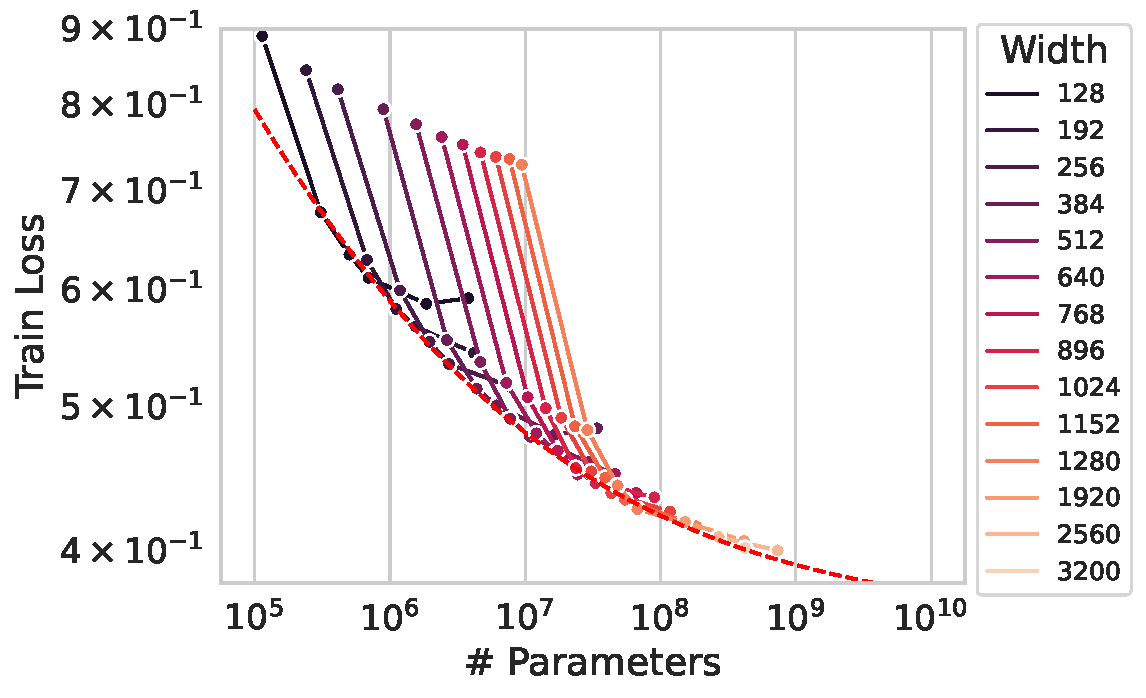
\includegraphics[width=0.52\linewidth]{figures/pareto_optimal_parameters_conv_cifar10.pdf}}
    \subfigure[Optimal Intermediate Depths]{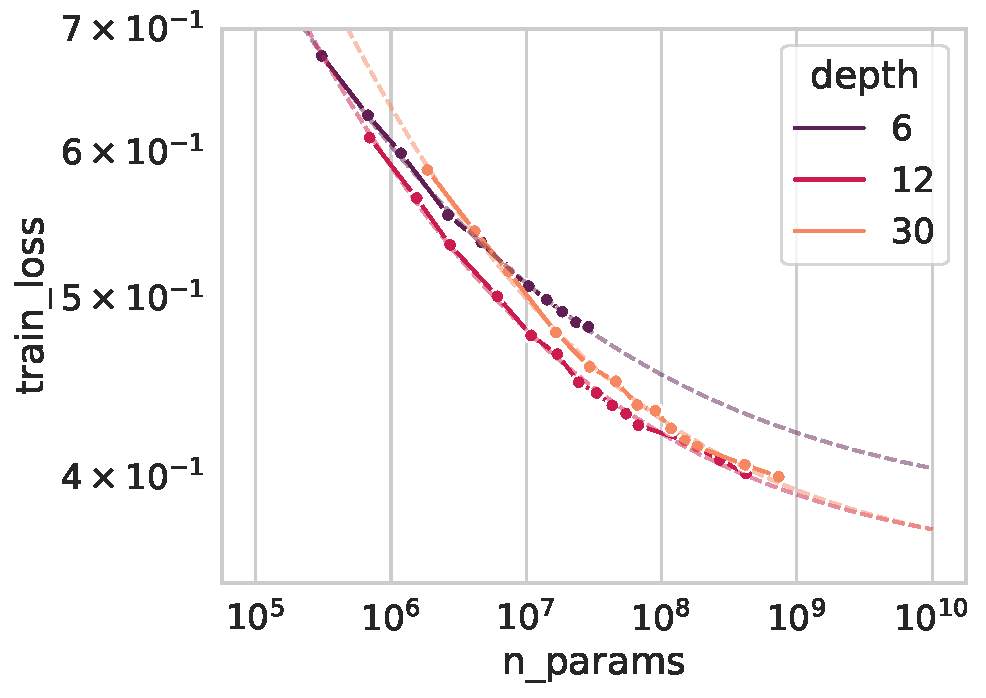
\includegraphics[width=0.45\linewidth]{figures/pareto_optimal_parameters_conv_cifar10_depth.pdf}}
    \caption{ Since all models have hyperparameter transfer across depths and widths, one can explore a trade-off between depth and width at the optimal learning rate. We illustrate this idea with a simple experiment on CIFAR-10. (a) We plot the final train loss as a function of parameters for different widths.  (b) intermediate depth of $\sim 9-12$ is preferred at fixed parameter count.   }
    \label{fig:param_envelope}
\end{figure}

\begin{figure}[h]
    \centering
    \subfigure[ResNet, SP]{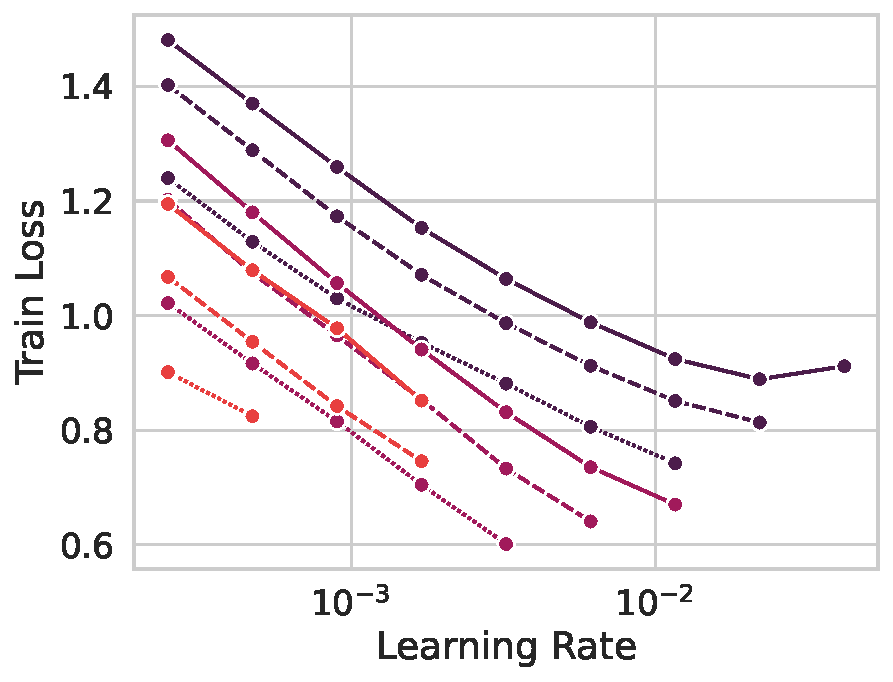
\includegraphics[width=0.4\linewidth]{figures/conv_cifar10_sp_small.pdf}}
    \subfigure[$\frac{1}{\sqrt L}$ ResNet SP]{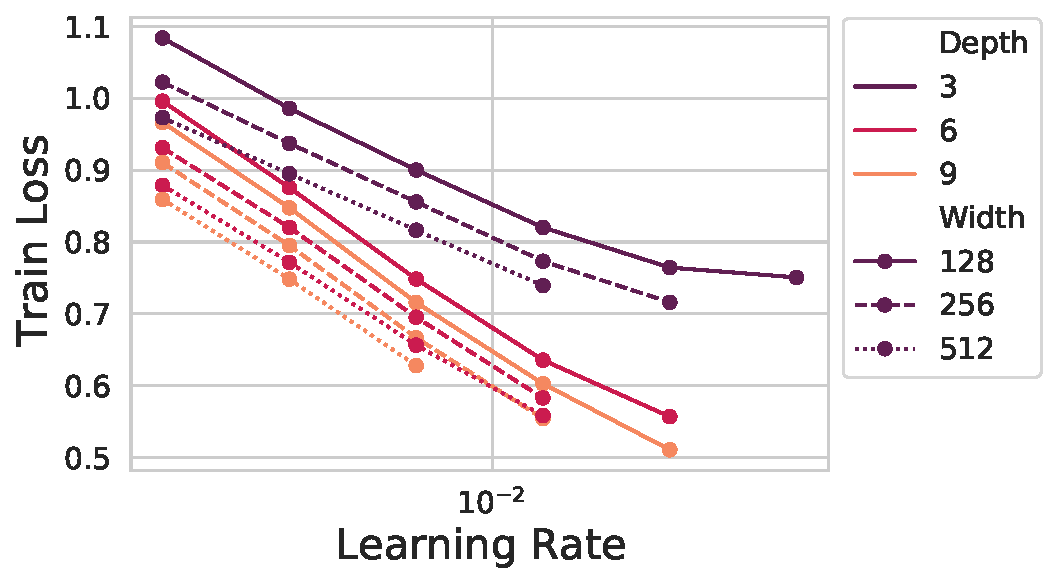
\includegraphics[width=0.55\linewidth]{figures/SP_sqrtL_LR_transfer.pdf}}
    % 
    \caption{Learning rates transfer across both depth and width in our proposed parameterization but not in standard parameterization (SP) or $\mu$P. Loss is plotted after $20$ epochs on CIFAR-10. %Points not shown represent divergences. 
    {\it All the missing datapoints indicate that the corresponding run diverged.} In particular, all depth $30$ runs diverged when using $\mu$P without $1/\sqrt{\text{depth}}$ scaling. }
    \label{fig:lr-transfer-sp}
\end{figure}

\subsection{How Long Should you Train for Accurate Transfer?}
An important question is after how many steps the optimal hyperparameters are fixed and can hence be selected without training for longer. In Fig.~\ref{fig:lr-dynamics}(a), we plot the training loss profiles for two different depths and 4 different learning rates for a residual convolutional network of width $512$ trained on CIFAR-10. Notice how after the first few epochs it is already possible to decide the optimal learning rate. We confirm this for a ViT trained on Tiny ImageNet in Fig.~\ref{fig:lr-dynamics}(b-c), where the optimal learning rate at two selected epochs (3 and 9) is the same. 

\begin{figure}[h]
    \centering
    \subfigure[LR dynamics]{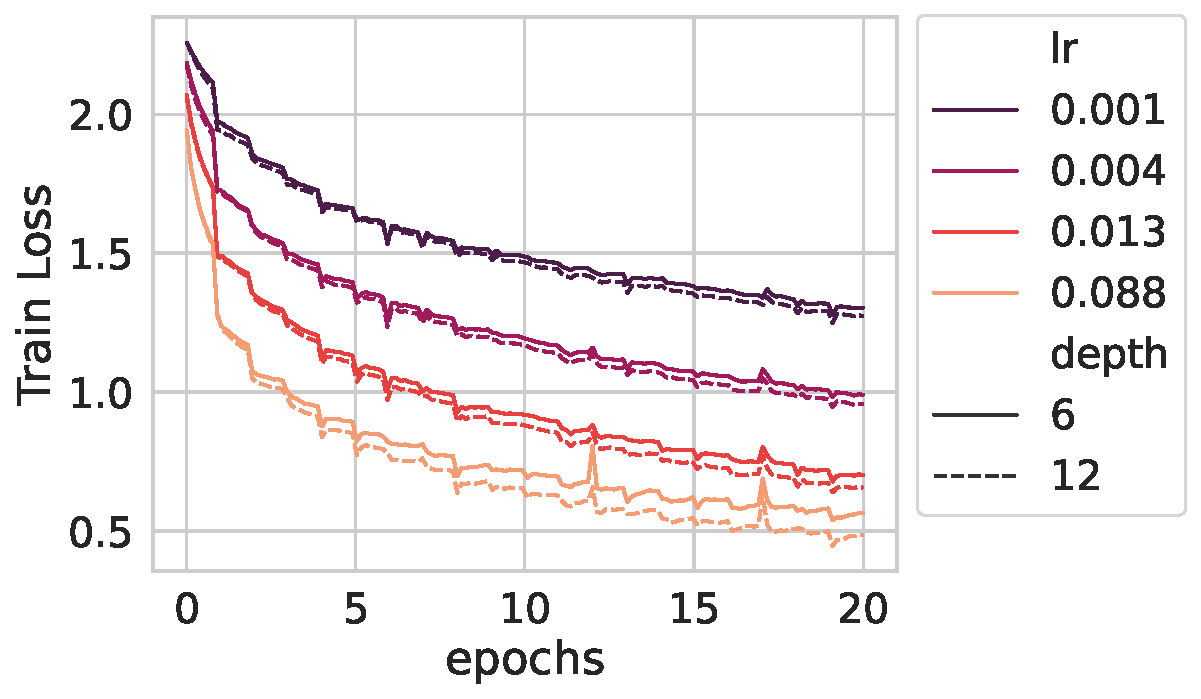
\includegraphics[width=0.37\linewidth]{figures/conv_cifar10_res_scaling_small_lr_dynamics.pdf}}
    \subfigure[Epoch 3]{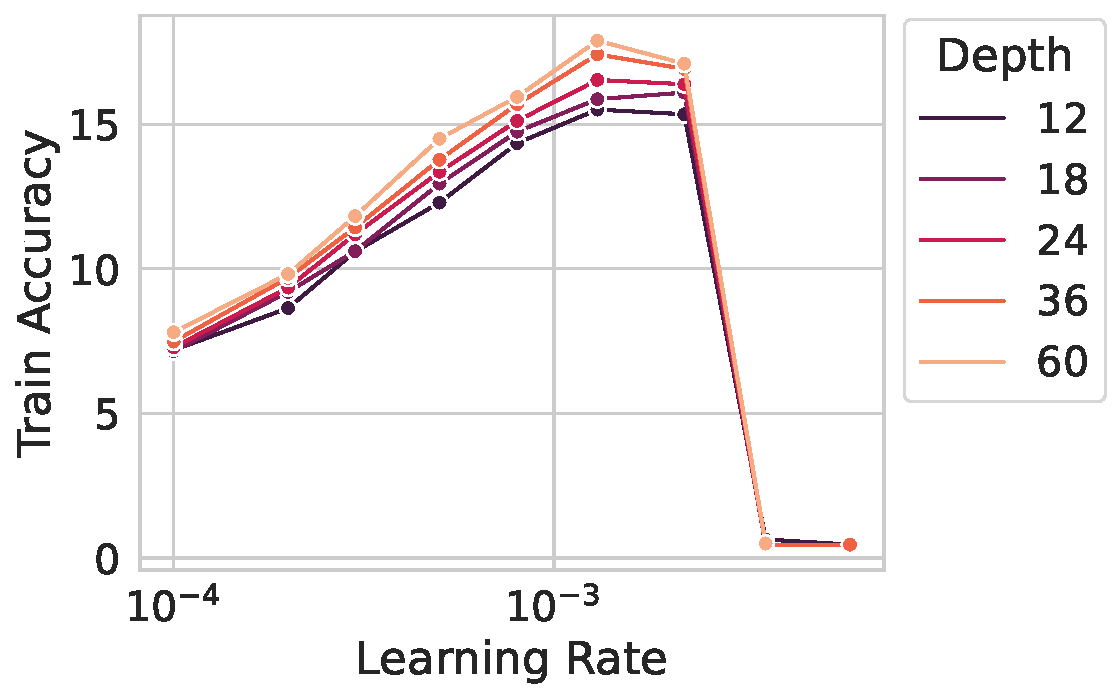
\includegraphics[width=0.34\linewidth]{figures/tiny_imgnet_vit_res_scaling_results_wu_1000_epoch3.pdf}}
    \subfigure[Epoch 9]{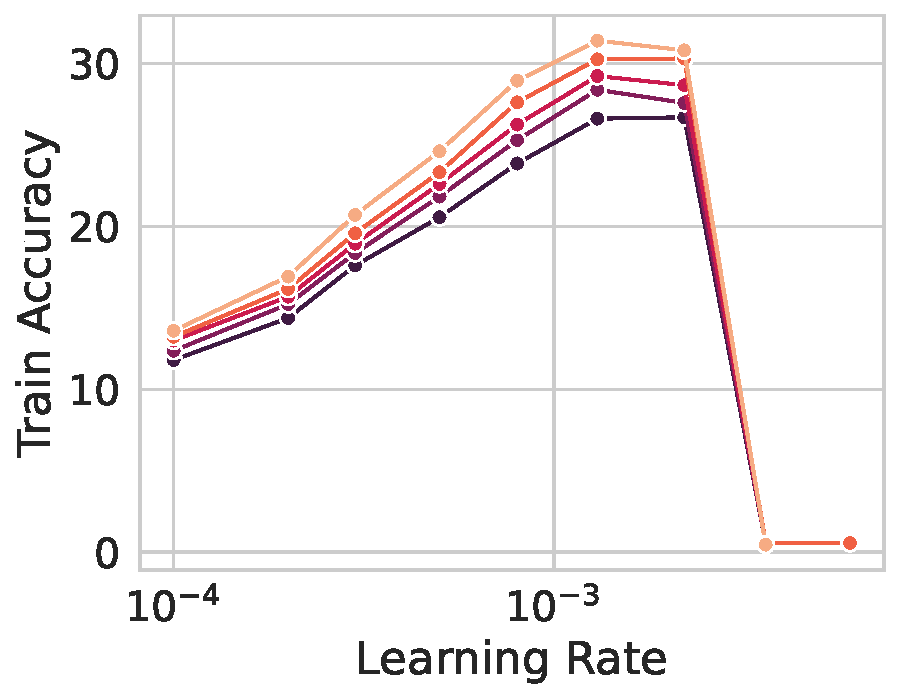
\includegraphics[width=0.27\linewidth]{figures/tiny_imgnet_vit_res_scaling_results_wu_1000_epoch9.pdf}} 
    \caption{(a) dynamics of train loss for different depths and learning rates. The network is the residual convolutional network trained on CIFAR-10. (b-c) learning rate tranfer plots for the same ViT at two different checkpoints (epoch $3$ and $5$). Notice how the optimal learning rate is determined after the first few epochs of training.}
    \label{fig:lr-dynamics}
\end{figure}

\subsection{Other Experiments}
In Fig.~\ref{fig:lr-transfer-sp}, we show how the learning rate does not transfer under SP for the residual model considered in this work, both with and without the $1/\sqrt{L}$-scaling.
%
In Fig.~\ref{fig:lr-transfer-norm-layers-ln}, we train models from the ResNets family, replacing BatchNorm with LayerNorm, concluding that the version with $1/\sqrt{L}$ scaling exhibits a better transfer.
%
In Fig.~\ref{fig:ImageNet_expts} we show our results on learning rate transfers for ImageNet, and in Fig.~\ref{fig:weight-decay}, we show how also weight decay transfer under the proposed $1/\sqrt{L}$-scaling and has very consistent dynamics. The model used is the simplified residual convolutional model, trained for 20 epochs on CIFAR-10.  

\begin{figure}[h]
    \centering
    \subfigure[ResNet + $\mu$P, LayerNorm]{\includegraphics[width=0.4\linewidth]{figures/ResNet_cifar10_no_res_scaling_ln.pdf}}
    \subfigure[$\frac{1}{\sqrt L}$ ResNet + $\mu$P, LayerNorm]{\includegraphics[width=0.52\linewidth]{figures/ResNet_cifar10_res_scaling_ln.pdf}}

    \caption{Effect of normalization layers. The above examples are taken after $20$ epochs on CIFAR-10. Normalization layers can slightly improve consistency across depths in standard ResNets, but consistency is much more reliable with the $1/\sqrt L$ scaling. }
    \label{fig:lr-transfer-norm-layers-ln}
\end{figure}

\begin{figure}[t!]
    \centering
    \subfigure[ResNet + $\mu$P, BatchNorm]{\includegraphics[width=0.42\linewidth]{figures/ResNet_cifar10_no_res_scaling_bn.pdf}}
    \subfigure[$\frac{1}{\sqrt L}$ ResNet + $\mu$P, BatchNorm]{\includegraphics[width=0.54\linewidth]{figures/ResNet_cifar10_res_scaling_bn.pdf}}
    \caption{Effect of normalization layers. The above examples are taken after $20$ epochs on CIFAR-10. Normalization layers can slightly improve consistency across depths in standard ResNets, but consistency is much more reliable with the $1/\sqrt L$ scaling. }
    \label{fig:lr-transfer-norm-layers-bn-width-depth}
\end{figure}

\begin{figure}[h]
    \centering
    \subfigure[Dynamics]{\includegraphics[width=0.46\linewidth]{figures/ImageNet_5_epoch_dynamics.pdf}}
    \subfigure[Learning Rate Transfer]{\includegraphics[width=0.43\linewidth]{figures/ImageNet_5_epoch_lr_transfer.pdf}}
    %\includegraphics[width=0.4\linewidth]{figures/ResNet_one_epoch_ImageNet_consistent_dynamics.pdf}
    %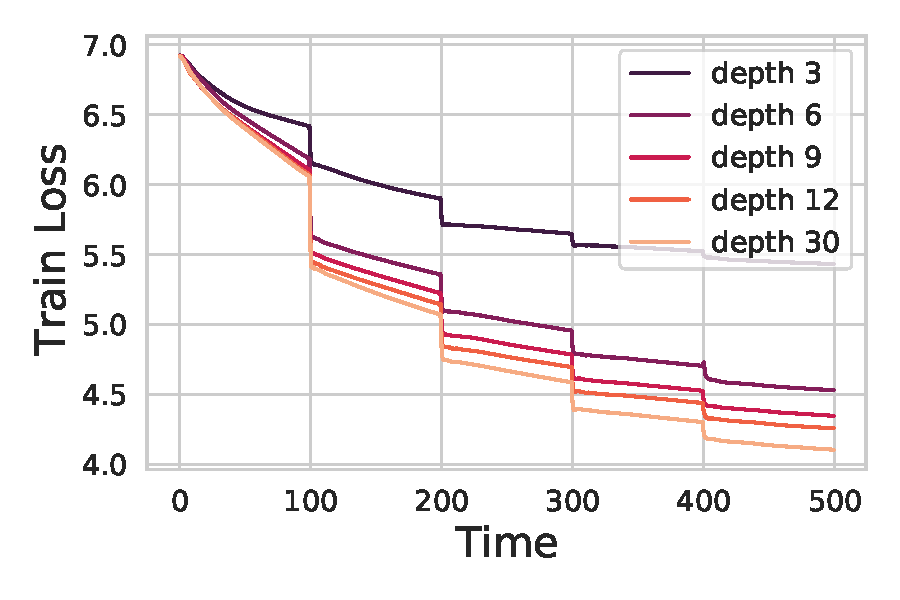
\includegraphics[width=0.4\linewidth]{figures/imgnet_epochs_5_loss_curves_time.pdf}    
    %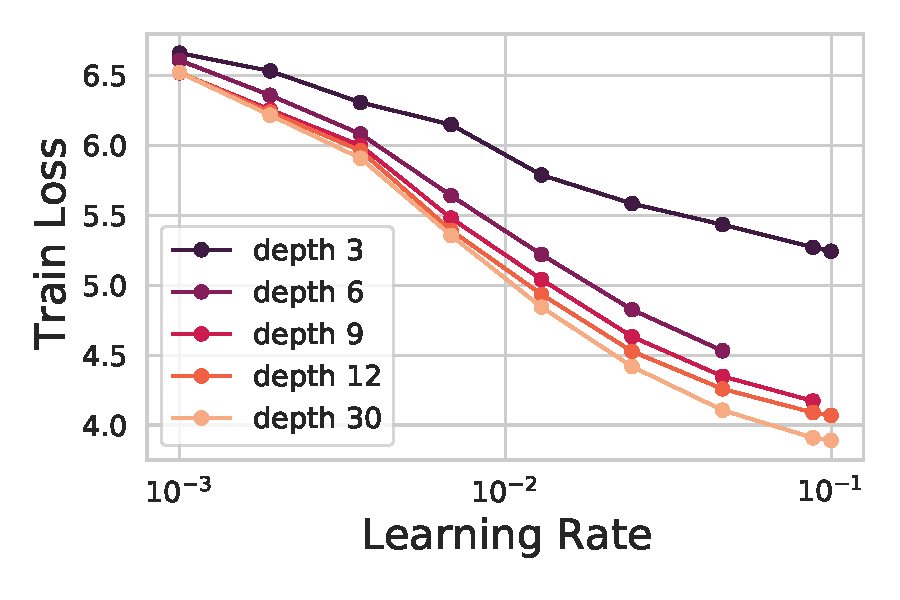
\includegraphics[width=0.4\linewidth]{figures/imgnet_lr_sweep_5_loss_epoch.pdf}
    %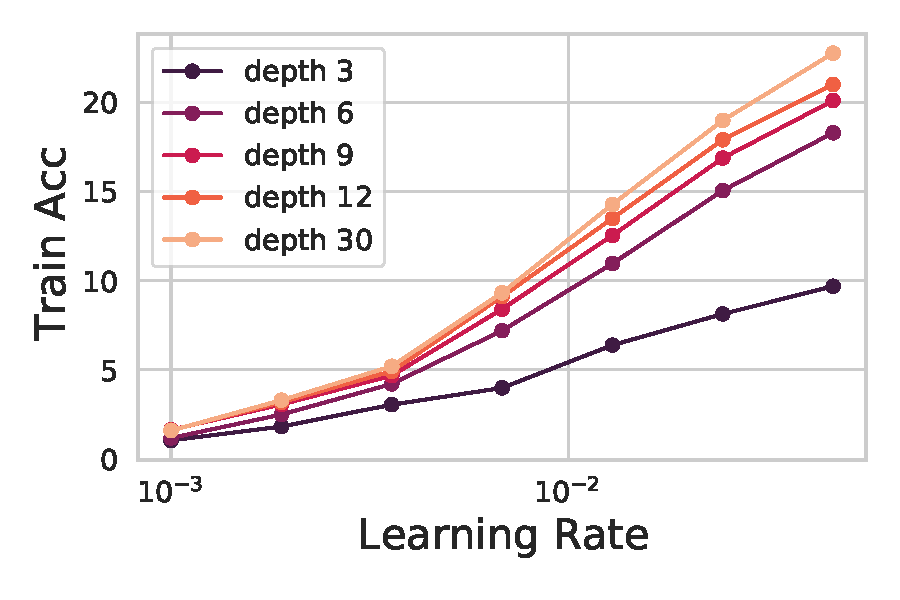
\includegraphics[width=0.32\linewidth]{figures/imgnet_lr_sweep_5_acc_epoch.pdf}
    \caption{Learning rate + depth sweep on ImageNet for $5$ epochs with depth extrapolations of ResNet-18 \emph{without any normalization layers}. Training is performed with SGD with momentum $0.9$ and batchsize $128$. (a) The loss curves for different learning rates (each learning rate is a distinct linestyle) and for different depths (colors). Dynamics are strikingly consistent across depths for each learning rate.  (b) The optimal learning rate is preserved across depths. }
    \label{fig:ImageNet_expts}
\end{figure}


\begin{figure}[h]
    \centering
    \subfigure[Fixed $L$ Convergence in $N$]{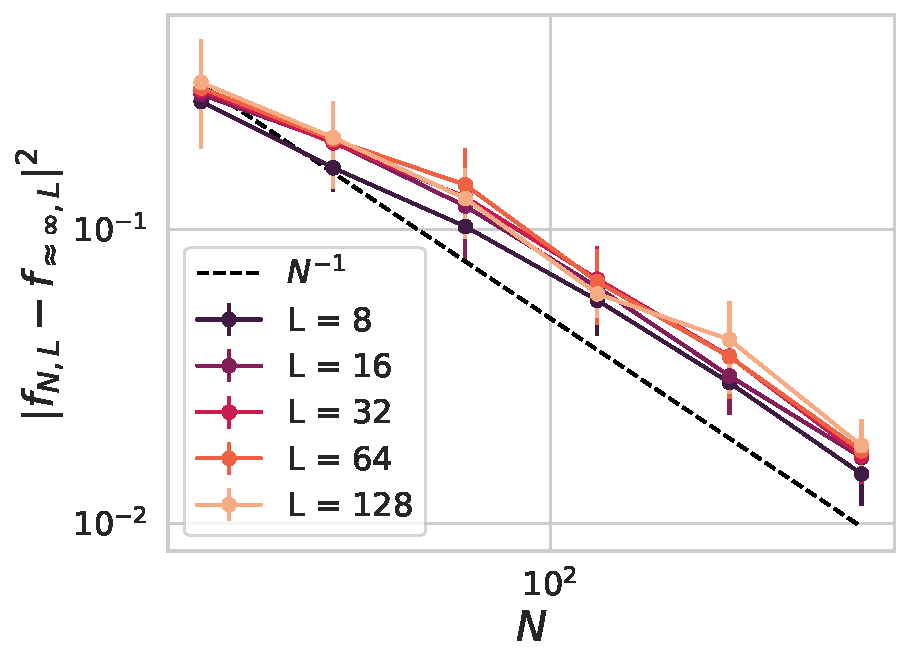
\includegraphics[width=0.32\linewidth]{figures/early_time_convergence_L_N_varyN_CIFAR_larger_batch_28_beta_1.5.pdf}}
    \subfigure[Average Square Error]{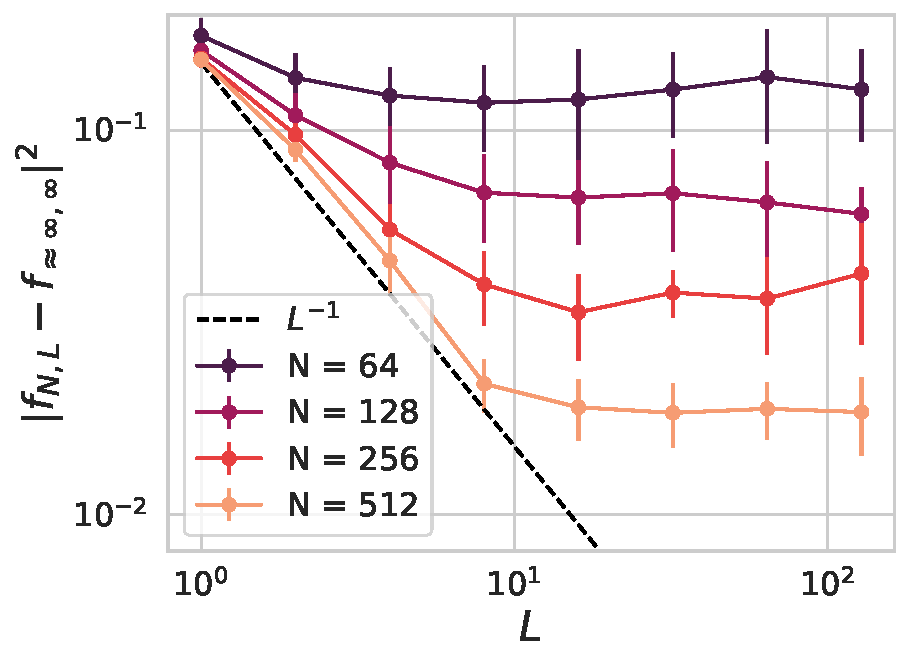
\includegraphics[width=0.32\linewidth]{figures/early_time_convergence_L_N_CIFAR_larger_batch_28_beta_1.5.pdf}}
    \subfigure[Error of Ensembled Logits]{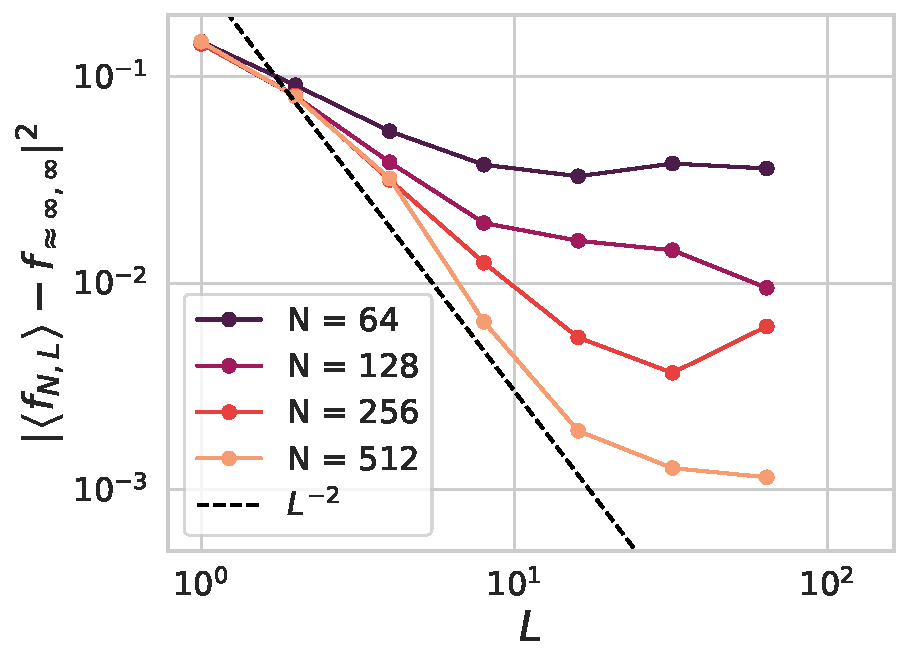
\includegraphics[width=0.32\linewidth]{figures/early_time_mean_log_convergence_L_N_CIFAR_larger_batch_28_beta_1.5.pdf}} 
    \caption{Further numerical support of our finite $N,L$ error decomposition in Appendix \ref{app:finite_N_L_error_analysis} through ensembling logits over $E=15$ random seeds in the same experimental setting as Figure \ref{fig:L_N_convergence plots}. (a) At each depth $L$, the finite width $N$ network converges in square error as $\mathcal{O}_{N,L}(N^{-1})$, independent of $L$. (b) The full expected square error from Figure \ref{fig:L_N_convergence plots} shows a convergence rate of $\mathcal{O}(L^{-1})$ for sufficiently large $N$, consistent with theory. (c) The ensemble averaged logits $\left< f_{L,N} \right>$ converge to the infinite depth proxy at a faster rate, which is consistent with the theoretical $\mathcal{O}(L^{-2})$ for sufficiently large $N$. }
    \label{fig:app_ensemble_convergence_rate}
\end{figure}


\begin{figure}[h]
    \centering
    \subfigure[Weight Decay Dynamics]{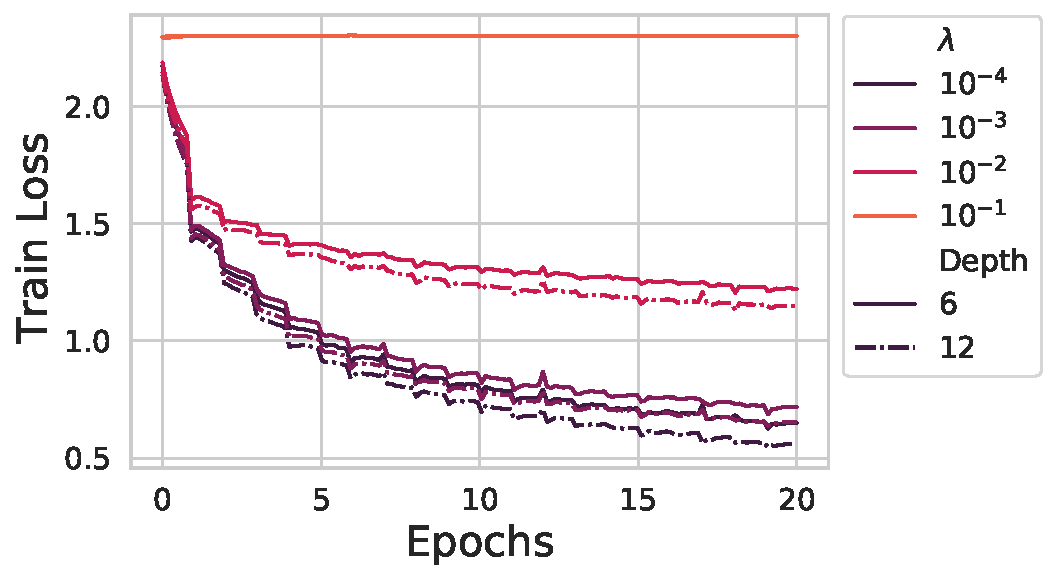
\includegraphics[width=0.5\linewidth]{figures/weight_decay_transfer_dynamics.pdf}}
    \subfigure[Final Loss vs Depth]{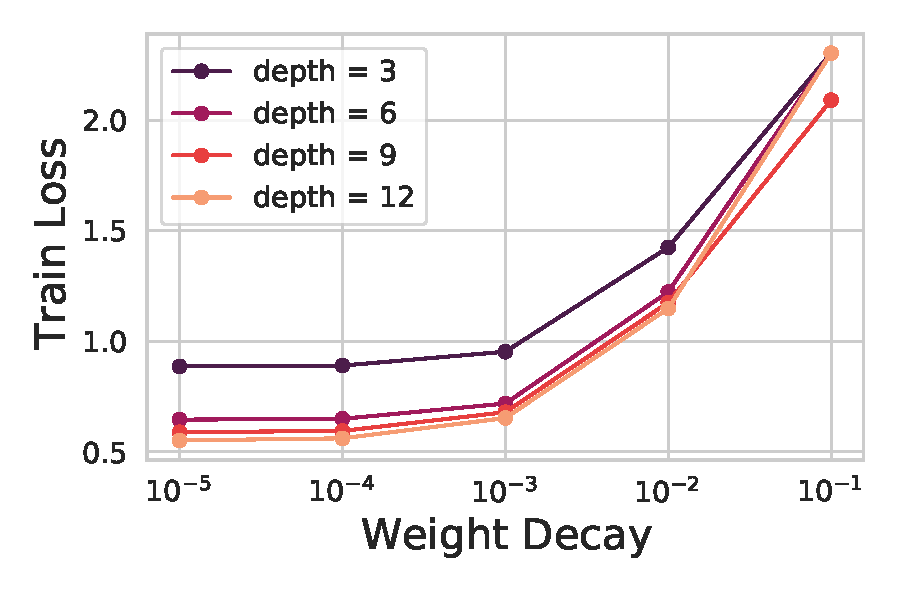
\includegraphics[width=0.425\linewidth]{figures/weight_decay_transfer.pdf}}
    \caption{Weight decay dynamics also transfer across depths. }
    \label{fig:weight-decay}
\end{figure}

\pagebreak
\pagebreak

\section{A Review of Various Width Parameterizations}

In this section, we discuss various parameterizations of neural networks with respect to the width of the model. We will discuss and compare their large width behaviors. First we will discuss the Neural-Tangent parameterization (NTP) which gives rise to a kernel limit. Next, we will discuss the Mean Field /$\mu$P parameterization which allows for feature learning at infinite width. In all models, we focus on 
\begin{align}
    f = \frac{1}{\sqrt{N} \gamma} \w^L \cdot \phi(\h^L) 
\end{align}
The choice of whether one is in NTP or $\mu$P depends on how $\gamma$ is scaled with respect to $N$. When training with a learning rate $\eta = \gamma^2 \eta_0$ (to ensure $\frac{d}{dt} f|_{t=0} = \mathcal{O}_\gamma(1)$), we have the following scale of internal preactivation updates \citep{bordelon2022self}
\begin{align}
    \frac{d}{dt} \h^\ell = \mathcal{O}(\gamma N^{-1/2}) .
\end{align}
Depending on how $\gamma$ is scaled with $N$, we can either have vanishing, constant, or diverging feature learning with respect to width $N$. In discrete time, a diverging parameterization is \textit{unstable} \citep{yang2021tensor}. Below we discuss two of the popular stable scalings for analysis.

\subsection{Neural Tangent Parameterization}
In NTP, the parameter $\gamma = \mathcal{O}_N(1)$ is a constant with respect to width $N$. As a consequence finite width $N$ models only exhibit $\mathcal{O}(N^{-1/2})$ movement of preactivations and $\mathcal{O}(N^{-1})$ movement of kernels. In this parameterization, models at very large width are well approximated by a kernel method \citep{jacot2018neural, lee2019wide}.
 
\subsection{Mean Field/$\mu$P Parameterizations}

On the other hand, if $\gamma=\gamma_0 \sqrt{N}$ for some constant $\gamma_0$, then the network converges to a feature learning infinite width limit. This is precisely the mean-field/$\mu$P parameterization \citep{yang2021tensor, bordelon2022self, bordelon2022influence}. The work of \cite{yang2021tensor} also gives a precise sense in which this parameterization is \textit{maximal}: each layer is learning features so that the preactivations in the sense that
\begin{align}
    \frac{1}{\sqrt N} \left( \frac{d}{dt} \W^\ell \right) \phi(\h^\ell) = \mathcal{O}(1)
\end{align}
Thus, the dynamics for $\frac{d}{dt} \h^{\ell+1} = \frac{d}{dt} \h^\ell +  \frac{1}{\sqrt N} \left( \frac{d}{dt} \W^\ell \right) \phi(\h^\ell) + \frac{1}{\sqrt N} \W^\ell \left(\frac{d}{dt} \phi(\h^\ell) \right) = \mathcal O_N(1)$. Because the underlying feature learning updates within the network are approximately constant as width $N$ is increased, this model exhibits more consistent dynamics and better hyperparameter transfer across widths \citep{yang2022tensor, vyas2023featurelearning}. 

We note that the code for $\mu$P released in the paper by \cite{yang2022tensor} uses an equivalent version of this dynamical system where learning rates do not need to be explictly scaled with $N$. 

\section{Derivation of the $N \to \infty$ limit at fixed $L$}\label{app:dmft_derivation_finite_L}

In this section, we characterize the feature learning dynamics of the $N \to \infty$ limit of fixed depth $L$ residual networks. Our derivation is an extension of the approach presented in \citep{bordelon2022self}. Before taking the limit, we first identify our order parameters and weight space dynamics. Then we take the $N \to \infty$ limit using a technique known as Dynamical Mean Field Theory (DMFT). 


\subsection{Finite $N,L$ Function and Weight Dynamics}
We start by computing the neural tangent kernel (NTK). For the sake of brevity, we will first write the equations where the read-in $\W^0$ weights are held fixed and will add their contribution to the dynamics in Appendix \ref{app:readin_readout}. Excluding these two weight matrices from the present discussion does not alter any of the scalings with width $N$ or depth $L$. The dynamics of the prediction $f$ under gradient flow take the form
\begin{align}
    \frac{d}{dt} f(\x;t) = \eta_0 \  \mathbb{E}_{\x'} K(\x,\x';t) \Delta(\x';t)
\end{align}
where $\Delta(\x;t) = - \frac{\partial \mathcal{L}(f(\x,t))}{\partial f(\x,t)}$ is an error signal and $K$ is the NTK of this model, which takes the form
\begin{align}
    K(\x,\x') = \gamma_0^2 N \sum_{\ell=1}^L \frac{\partial f(\x)}{\partial \W^{\ell}} \cdot \frac{\partial f(\x')}{\partial \W^{\ell}} . 
\end{align}
Explicitly calculating the gradients of the output with respect to the weights $\W^\ell$ gives
\begin{align}
    N \gamma_0 \frac{\partial f(\x)}{\partial \W^\ell} = \frac{1}{\sqrt{N L }} \g^{\ell+1}(\x) \phi(\h^\ell(\x))^\top \ , \ g_i^{\ell} \equiv N \gamma_0 \frac{\partial f(\x)}{\partial h_i^{\ell}(\x)} \sim \mathcal{O}_{N,L}(1) 
\end{align}
Using this above formula, we find that the NTK is $\mathcal{O}(1)$ with respect to $N, L$ 
\begin{align}
    K(\x,\x') = \frac{1}{L} \sum_{\ell=1}^{L}  G^{\ell+1}(\x,\x') \Phi^\ell(\x,\x')
\end{align}
where we introduced the $\mathcal{O}(1)$ feature kernel $\Phi^\ell$ and gradient kernels $G^\ell$ which have the form
\begin{align}
    \Phi^\ell(\x,\x') = \frac{1}{N} \phi(\h^\ell(\x)) \cdot \phi(\h^\ell(\x')) \ , \ G^{\ell}(\x,\x') = \frac{1}{N} \g^\ell(\x) \cdot \g^\ell(\x')
\end{align}
The base cases for the feature and gradient kernels are given by
\begin{align}
    \Phi^0(\x,\x') = \frac{1}{D} \x \cdot \x' \ , \ G^{L+1}(\x,\x') = 1 .
\end{align}

We next start by computing the dynamics of the weights under gradient flow
\begin{align}
    \frac{d}{dt} \W^{\ell} = \frac{\eta_0 \gamma_0}{\sqrt{L N}} \ \mathbb{E}_{\x} \ \Delta(\x;t) \g^{\ell+1}(\x,t) \phi(\h^\ell(\x,t))^\top  .
\end{align}
Integrating this equation from time $0$ to time $t$, we get the following 
\begin{align}
    \h^{\ell+1}(\x,t) =& \h^{\ell}(\x,t) + \frac{1}{\sqrt{N L}} \W^\ell(0) \phi(\h^\ell) \nonumber
    \\
    &+ \frac{\eta_0 \gamma_0}{L} \int_0^t ds \mathbb{E}_{\x'} \Delta(\x',s) \g^{\ell+1}(\x',s) \Phi^{\ell}(\x,\x';t,s)
\end{align}
where $\Phi^{\ell}(\x,\x';t,s) = \frac{1}{N} \phi(\h^\ell(\x,t)) \cdot \phi(\h^\ell(\x';s))$ is the double time-index generalization of the feature kernel. Similarly, we obtain a backward pass relation of the form
\begin{align}
    \g^{\ell}(\x,t) =& \g^{\ell+1}(\x,t) + \frac{1}{\sqrt{NL}} \dot\phi(\h^\ell(\x,t)) \odot  \W^{\ell}(0)^\top \g^{\ell+1} \nonumber
    \\
    &+ \frac{\eta_0 \gamma_0}{L}  \dot\phi(\h^\ell(\x,t)) \odot  \int_0^t ds   \mathbb{E}_{\x'} \Delta(\x',s)  G^{\ell+1}(\x,\x';t,s) \phi(\h^\ell(\x',s))
\end{align}

These equations define update rules for the preactivations $\h^\ell$ and the gradients $\g^\ell$ in terms of the feature and gradient kernels $\{ \Phi^\ell,  G^{\ell} \}$. However the above equations explicitly depend on the random initial weights $\W^\ell(0)$ through which time-varying signals propagate. Our ultimate goal is to gain insight into the effective dynamics over random initializations in the large $N$ limit. To do that, we will invoke dynamical mean field theory. In the next section, we characterize how these terms behave at large $N$ using a saddle point argument. 

\subsection{Intuitive Explanation of Large Width Feature Learning Limit}

In the limit of $N \to \infty$ with $\gamma_0$ held fixed, the above equations can be simplified. The two key effects that occur at large width are
\begin{itemize}
    \item Kernels (feature kernels, gradient kernels, NTK) and output logits concentrate by a law of large numbers.
    \item At each layer, each of the hidden neuron's activities becomes independent draws from a \textit{single site stochastic process} which is characterized by the kernels. 
\end{itemize}
Once the single site density is known, the kernels can be computed as averages over the single site density. The next section derives this result formally from a Martin-Siggia-Rose Path Integral derivation of the Dynamical Mean Field Theory \citep{martin1973statistical}. 

\subsection{Path-integral and Saddle Point Equations in $N \to \infty$ Limit}

This computation sketches the DMFT derivation of the limiting large $N$ process. Examples of detailed computations of the DMFT action $\mathcal S$ can be found in the Appendix of \cite{bordelon2022self, bordelon2022influence}. Our notation is chosen to match the derivations found in their Appendix. 

To characterize the effect of the random initial weights, we will attempt to characterize the distribution of $\h^\ell(\x,t), \g^\ell(\x,t)$ by tracking the moment generating functional of these fields 
\begin{align}
    Z[\{ \bm j^h, \bm j_g \}] = \mathbb{E}_{\{\W^\ell(0) \}} \exp\left( \sum_{\ell=1}^L \int d\x \int dt \  [ \bm j_h^\ell(\x,t) \cdot \h^\ell(\x,t) + \bm j_g(\x,t) \cdot \g^\ell(\x,t) ] \right)
\end{align}
Moments of the fields can be obtained with differentiation near zero source, for example
\begin{align}
    \lim_{\{\bm j_h^\ell,\bm j_g^\ell\} \to 0} \frac{\delta}{\delta j^\ell_{h, i_1}(\x_1,t_1) } ... \frac{\delta}{\delta j^\ell_{h, i_k}(\x_k,t_k) } Z[\{ \bm j^h, \bm j_g \}] = \left< h_{i_1}^{\ell_1}(\x_1,t_1) ... h_{i_k}^{\ell_k}(\x_k,t_k) \right> .
\end{align}
Now, following \cite{bordelon2022self}, we introduce the following useful auxiliary fields
\begin{align}
    \bm\chi^{\ell+1}(\x,t) = \frac{1}{\sqrt N} \W^{\ell}(0) \phi(\h^\ell(\x,t)) \ , \  \bm\xi^{\ell}(\x,t) = \frac{1}{\sqrt N} \W^{\ell}(0)^\top \g^{\ell+1}(\x,t)
\end{align}
The choice to introduce these auxiliary fields is apparent once one realizes that the $h$ and $g$ fields can be regarded as functions of $\chi, \xi$ and the kernels $\Phi, G$. We enforce the constraints defining these fields with Dirac-delta functions by repeatedly multiplying by unity
\begin{align}
    1 &= \int d \bm\chi^{\ell+1}(\x,t) \  \delta\left( \bm\chi^{\ell+1}(\x,t) - \frac{1}{\sqrt N} \W^\ell(0) \phi(\h^\ell(\x,t))  \right) \nonumber
    \\
    &= \int \frac{  d \hat{\bm\chi}^{\ell+1}(\x,t) d\bm\chi^{\ell+1}(\x,t) }{(2\pi)^N} \exp\left( i \hat{\bm\chi}^{\ell+1}(\x,t) \cdot \left[\bm\chi^{\ell+1}(\x,t) - \frac{1}{\sqrt N} \W^\ell(0) \phi(\h^\ell(\x,t))  \right]\right)
\end{align}
for all $\ell,\x,t$. And similarly for the $\g^\ell$ fields. After this insertion, the averages over $\{\W^\ell(0)\}$ can be performed with Gaussian integration. Concretely, we obtain the following average over Gaussian initialization $\W^\ell(0)$
\begin{align}
    &\ln \mathbb{E}\exp\left( - \frac{i}{\sqrt N} \text{Tr} \ \W^\ell(0)^\top  \int d\x \int dt \left[ \bm{\hat\chi}^{\ell+1}(\x,t) \phi(\h^\ell(\x,t))^\top + \g^{\ell+1}(\x,t) \bm\xi^\ell(\x,t)^\top  \right]  \right) \nonumber
    \\
    =& -\frac{1}{2} \int dt ds  d\x d\x' \ \bm{\hat \chi}^{\ell+1}(\x,t) \cdot \bm{\hat \chi}^{\ell+1}(\x',s) \Phi^{\ell}(\x,\x';t,s) \nonumber
    \\
    &- \frac{1}{2} \int dt ds  d\x d\x' \ \bm{\hat \xi}^\ell(\x,t) \cdot \bm{\hat \xi}^\ell(\x',s) G^{\ell+1}(\x,\x';t,s) \nonumber
    \\
    &- i \int dt ds  d\x d\x' \ \bm{\hat \chi}^{\ell+1}(\x,t) \cdot \g^{\ell+1}(\x',s) \ A^{\ell}(\x,\x';t,s)
\end{align}
where we introduced the following order parameters
\begin{align}
    \Phi^{\ell}(\x,\x';t,s) &= \frac{1}{N} \phi(\h^\ell(\x,t)) \cdot \phi(\h^\ell(\x',s))  \ , \ G^{\ell}(\x,\x';t,s) = \frac{1}{N} \g^\ell(\x,t) \cdot \g^\ell(\x',s) 
    \\
     A^{\ell}(\x,\x';t,s) &= - \frac{i}{N} \phi(\h^\ell(\x,t)) \cdot \bm{\hat\xi}^\ell(\x',s)
\end{align}
As we did with the $\bm\chi,\bm\xi$ fields, we can enforce the definition of the above order parameters with integral representations of Dirac-delta functions. For example, the $\Phi$ kernels can be enforced by inserting 
\begin{align}
    1 = \int \frac{d \Phi^{\ell}(\x,\x';t,s) d \hat \Phi^{\ell}(\x,\x';t,s)}{2\pi i N^{-1}} &\exp\left( N \Phi^{\ell}(\x,\x';t,s) \hat \Phi^{\ell}(\x,\x';t,s) \right) \nonumber
    \\
    &\exp\left( - \hat \Phi^{\ell}(\x,\x';t,s)  \phi(\h^\ell(\x,t)) \cdot \phi(\h^\ell(\x',t')) \right)
\end{align}
where the $\hat\Phi$ integral is performed along the imaginary axis $(-i \infty, i\infty)$ in the complex plane. The same trick is performed for $G^\ell$ and $A^\ell$ which have conjugate variables $\hat G^\ell, B^\ell$ respectively. After inserting these new variables, we find that the moment generating function can be expressed as an integral over a collection of order parameters $\bm q$,
\begin{align}
    \bm q = \text{Vec}\{ \Phi^\ell(\x,\x';t,s) , \hat\Phi^\ell(\x,\x';t.s) , G^\ell(\x,\x',t,s), 
    \hat G^\ell(\x,\x',t,s),  A^{\ell}(\x,\x',t,s) B^{\ell}(\x,\x',t,s)  \},
\end{align}
which is vectorized over all layers $\ell$ time points $t,s$ and samples $\x,\x'$. The moment generating function takes the form
\begin{align}
    Z[\{\bm j_h, \bm j_g\}] = \int d\bm q \exp\left( N \mathcal S[\bm q, \bm j_h, \bm j_g] \right)
\end{align}
where $\mathcal S$ is the $\mathcal{O}_N(1)$ DMFT action which has the following form
\begin{align}
    \mathcal S = &\sum_{\ell} \int d\x d\x' dt ds \left[ \Phi^\ell(\x,\x';t,s) \hat\Phi^\ell(\x,\x';t.s) + G^\ell(\x,\x',t,s)
    \hat G^\ell(\x,\x',t,s) \right] \nonumber
    \\
    &-\sum_{\ell} \int d\x d\x' dt ds \  A^{\ell}(\x,\x',t,s) B^{\ell}(\x',\x,s,t) + \frac{1}{N} \sum_{i=1}^N \mathcal{Z}_i[\bm q, \bm j_h, \bm j_g]
\end{align}
The functions $\mathcal Z_i$ are \textit{single-site} moment generating functions (MGFs) which express the distribution of $h_i, g_i$ for a given value of the order parameters $\bm q$ and sources $\bm j_h, \bm j_g$. 
\begin{align}
    \mathcal Z_i = \int \prod_{\ell, \x,t} d\hat{\chi}^\ell(\x,t) d\hat{\chi}^\ell(\x,t) d\hat{\chi}^\ell(\x,t) d\hat{\chi}^\ell(\x,t) \exp\left( - \sum_\ell \mathcal{H}_i^\ell[\hat\chi, \hat\xi,\chi,\xi, j_{h,i} , j_{g,i}] \right)   
\end{align}
where $\mathcal H_i^\ell$ are the single-site Hamiltonians
\begin{align}
    \mathcal H_i^\ell =& \frac{1}{2} \int d\x d\x' dt ds \left[ \Phi^{\ell-1}(\x,\x';t,s) \hat\chi^{\ell}(\x,t) \hat\chi^{\ell}(\x',s)  +  G^{\ell+1}(\x,\x';t,s) \hat\xi^{\ell}(\x,t) \hat\xi^{\ell}(\x',s)    \right] \nonumber
    \\
    &+ \int d\x d\x' dt ds \left[ \hat \Phi^{\ell}(\x,\x';t,s) \phi(h^\ell(\x,t)) \phi(h^\ell(\x',t')) + \hat G^{\ell}(\x,\x';t,s) g^\ell(\x,t) g^\ell(\x',s)  \right] \nonumber
    \\
    &+ i \int d\x d\x' dt ds \left[ A^{\ell-1}(\x,\x';t,s) \hat\chi^\ell(\x,t) g^{\ell}(\x',s) + B^{\ell}(\x,\x';t,s) \hat\xi^\ell(\x,t) \phi(h^\ell(\x',s))   \right] \nonumber
    \\
    &- \int d\x dt  \left[ i \hat\chi^\ell(\x,t) \chi^\ell(\x,t) + i \hat\xi^\ell(\x,t) \xi^\ell(\x,t) + j_{h,i}^\ell(\x,t) h^\ell(\x,t) + j_{g,i}^\ell(\x,t) g^\ell(\x,t) \right] 
\end{align}
In the above formulas, the $h, g$ fields should be regarded as functions of the $\chi, \xi$ fields. 

Since the moment generating function has the form $Z = \int d\bm q \exp\left( N \mathcal S[\bm q] \right)$, the $N \to \infty$ limit can thus be characterized by the steepest-descent method (saddle-point integration over $\bm q$). The result is that all of the order parameters take on definite values (concentrate) at infinite width. The saddle point equations $\frac{\partial \mathcal S}{\partial \bm q} = 0$ state that each of the kernels takes on definite values
\begin{align}
    \Phi^\ell(\x,\x';t,s) &= \frac{1}{N} \sum_{i=1}^N \left< \phi(h^\ell(\x,t)) \phi(h^\ell(\x',s) ) \right>_{i} \nonumber
    \\ 
    G^\ell(\x,\x';t,s) &= \frac{1}{N} \sum_{i=1}^N \left< g^\ell(\x,t) g^\ell(\x',s) \right>_{i} \nonumber
    \\
    A^\ell(\x,\x';t,s) &=- \frac{i}{N} \sum_{i=1}^N \left< \phi(h^\ell(\x,t)) \hat \xi^\ell(\x',s)   \right>_i \nonumber 
    \\ 
    B^\ell(\x,\x';t,s) &= - \frac{i}{N} \sum_{i=1}^N \left< g^{\ell+1}(\x,t)  \hat\chi^{\ell+1}(\x',s)   \right>_i \nonumber
    \\
    \hat \Phi^\ell(\x,\x';t,s) &= - \frac{1}{2 N} \sum_{i=1}^N \left< \hat\chi^{\ell}(\x,t) \hat\chi^\ell(\x',s) \right>_{i} \nonumber
    \\ 
    \hat G^\ell(\x,\x';t,s) &= -  \frac{1}{2 N} \sum_{i=1}^N \left< \hat\xi^{\ell}(\x,t) \hat\xi^\ell(\x',s) \right>_{i}
\end{align}
where $\left< \right>_i$ denotes averaging over a \textit{single site stochastic process} defined by the moment generating function $\mathcal Z_i$. At zero source $\bm j \to 0$ all of the single site MGF functions $\mathcal Z_i$ are identical so all averages $\left< \cdot \right>_i$ are also identical. At zero source, the kernels have the simple expressions such as $\Phi^\ell(\x,\x';t,s) =  \left< \phi(h^\ell(\x,t)) \phi(h^\ell(\x',s) ) \right>$. 

\subsubsection{Hubbard-Stratonovich transform}

Now that we know the kernels $\Phi^\ell, G^\ell$ take on definite values at $N \to \infty$, we can perform a Hubbard-Stratonovich transformation to introduce Gaussian sources
\begin{align}
    &\exp\left( - \frac{1}{2} \int d\x d\x' dt ds \  \hat\chi^\ell(\x,t) \hat\chi^\ell(\x',t') \Phi^{\ell-1}(\x,\x';t,s) \right) \nonumber 
    \\
    &= \left< \exp\left( - i \int d\x dt \  \hat\chi^\ell(\x,t) u^\ell(\x,t)   \right) \right>_{u^\ell \sim \mathcal{GP}(0,\Phi^{\ell-1})}
    \\
    &\exp\left( - \frac{1}{2} \int d\x d\x' dt ds \  \hat\xi^\ell(\x,t) \hat\xi^\ell(\x',t') G^{\ell+1}(\x,\x';t,s) \right) \nonumber 
    \\
    &= \left< \exp\left( - i \int d\x dt \  \hat\xi^\ell(\x,t) r^\ell(\x,t)   \right) \right>_{r^\ell \sim \mathcal{GP}(0,G^{\ell+1})}
\end{align}
After introducing these Gaussian sources $u^\ell, r^\ell$, we have linearized the single site Hamiltonians $\mathcal H_i^\ell$ with respect to $\hat\chi$ and $\hat\xi$. Integration over these variables gives us the following Dirac-Delta function constraints
\begin{align}
    \chi^\ell(\x,t) &= u^\ell(\x,t) + \int d\x ds \  A^{\ell-1}(\x,\x';t,s) g^{\ell}(\x',s) \nonumber
    \\
    \xi^{\ell}(\x,t) &= r^\ell(\x,t) + \int d\x ds \ B^\ell(\x,\x';t,s) \phi(h^\ell(\x',s))  
\end{align}
Using similar manipulations, we can simplify the expressions for $A^\ell, B^\ell, \hat\Phi, \hat G$ at zero source $\bm j = 0$
\begin{align}
    A^{\ell}(\x,\x';t,s) &= \left< \frac{\delta \phi(h^\ell(\x,t))}{\delta r^\ell(\x',s)} \right> \nonumber
    \\
    B^{\ell}(\x,\x';t,s) &= \left< \frac{\delta g^{\ell+1}(\x,t)}{\delta u^\ell(\x',s)} \right> \nonumber
    \\
    \hat\Phi^\ell(\x,\x';t,s) &= 0 \ , \ \hat G^\ell(\x,\x';t,s)  = 0
\end{align}
Plugging the dynamics for $\chi, \xi$ into the formulas for $h^\ell, g^\ell$, we obtain the following final equations for the stochastic process of $h^\ell, g^\ell$. 

\begin{subequations}
\begin{empheq}[box=\fbox]{align}
   h^{\ell+1}(\x,t) &= h^{\ell}(\x,t) + \frac{1}{\sqrt L} u^{\ell+1}(\x,t) + \frac{1}{\sqrt L} \int d\x' ds \ A^{\ell}(\x,\x';t,s) g^{\ell+1}(\x',s) \nonumber
    \\
    &+ \frac{\eta_0 \gamma_0}{L} \mathbb{E}_{\x'} \  \int_0^t ds \  \Delta(\x',s)  \Phi^{\ell}(\x,\x';t,s) \  g^{\ell+1}(\x',s) \ , \ u^\ell \sim \mathcal{GP}(0, \Phi^{\ell-1}) \nonumber
    \\
    g^{\ell}(\x,t) &= g^{\ell+1}(\x,t) + \frac{1}{\sqrt L} \dot\phi(h^\ell(\x,t)) z^\ell(\x,t) \nonumber \ , \ 
    \\
    z^\ell(\x,t) &= r^\ell(\x,t) +  \int d\x' ds \ B^\ell(\x,\x';t,s) \phi(h^\ell(\x',s)) \ , \ r^\ell \sim \mathcal{GP}(0, G^{\ell+1}) \nonumber
    \\
    &+ \frac{\eta_0 \gamma_0}{\sqrt L} \mathbb{E}_{\x'} \int_0^t ds \ \Delta(\x',s) G^{\ell+1}(\x,\x';t,s) \phi(h^\ell(\x',s)) 
\end{empheq}
\end{subequations}

where the order parameters satisfy the the following saddle point equations

\begin{subequations}
\begin{empheq}[box=\fbox]{align}
  &\Phi^\ell(\x,\x';t,s) =  \left< \phi(h^\ell(\x,t)) \phi(h^\ell(\x',s) ) \right>
    \ , \ G^\ell(\x,\x';t,s) =  \left< g^\ell(\x,t) g^\ell(\x',s) \right>\nonumber
    \\
    &A^{\ell}(\x,\x';t,s) = \left< \frac{\delta \phi(h^\ell(\x,t))}{\delta r^\ell(\x',s)} \right> 
    \ , \ B^{\ell}(\x,\x';t,s) = \left< \frac{\delta g^{\ell+1}(\x,t)}{\delta u^{\ell+1}(\x',s)} \right> \nonumber
    \\
    & \frac{d f(\x,t)}{dt} = \eta_0 \mathbb{E}_{\x'} K(\x,\x',t) \Delta(\x',t) 
 \ , \     \Delta(\x,t) = - \frac{\partial \mathcal L}{\partial f(\x,t)} \nonumber
    \\
    &K(\x,\x',t) = \frac{1}{L} \sum_{\ell=1}^L G^{\ell+1}(\x,\x';t,s) \Phi^{\ell}(\x,\x';t,s) 
\end{empheq}
\end{subequations}

Up to the residual skip connections and the factors of $\frac{1}{\sqrt L}$, this agrees with the $N \to \infty$ limit DMFT derived in \cite{bordelon2022self}. At fixed $L$ this above equation can be solved with a self-consistent Monte Carlo sampling procedure. For deep linear networks, the equations close since all $h, g$ fields are Gaussian. In the next section, we analyze the behavior of the above equations at large depth $L$ so that we can take a large depth limit. 



\section{The $L \to \infty$ limit from the DMFT Saddle Point Equations}\label{app:large_L_dmft}

In this section, we consider how the infinite width dynamics behaves at large depth. We will show that the limiting dynamics takes the form of a system of ODEs for the kernels in terms of layer time $\tau = \ell/ L$. First, we will show that the response functions need to be rescaled with respect to $L$. Then we will take a continuum limit over layers to arrive at the final ODEs for the $\Phi$ and $G$ correlation functions. 


\subsection{Unfolding the Layer Recursion}
A useful first step which we will use in the following analysis is ``unfolding" the recurrence to get explicit formulas for $h^\ell$ in terms of all of the Gaussian sources $u$ and all of the gradient fields $g^\ell$.     
\begin{align}
    h^\ell(\x,t) =& h^1(\x,t) + \frac{1}{\sqrt L} \sum_{k=0}^{\ell} u^{k}(\x,t) + \frac{1}{\sqrt L} \sum_{k=1}^{\ell-1} \int d\x' ds \ A^{k}(\x,\x';t,s) g^{k+1}(\x',s) \nonumber
    \\
    &+\frac{\eta_0 \gamma_0}{L}  \mathbb{E}_{\x'} \int_0^t ds \  \Delta(\x',s) \sum_{k=0}^{\ell-1} \Phi^k(\x,\x',t,s) g^{k+1}(\x',s) 
\end{align}
and similarly for the backward pass, we have
\begin{align}
    g^\ell(\x,t) =& g^L(\x,t) + \frac{1}{\sqrt L} \sum_{k=\ell}^{L} \dot\phi(h^k(\x,t)) r^{k}(\x,t) \nonumber
    \\
    &+ \frac{1}{\sqrt L} \sum_{k=\ell}^{L} \dot\phi(h^k(\x,t)) \int d\x' ds \ B^{k}(\x,\x';t,s)  \phi(h^k(\x',s)) \nonumber
    \\
    &+\frac{\eta_0 \gamma_0}{L}   \sum_{k=\ell}^{L} \dot\phi(h^k(\x,t)) \mathbb{E}_{\x'} \int_0^t ds \  \Delta(\x',s) \sum_{k=1}^{\ell-1} G^k(\x,\x',t,s) \phi(h^k(\x',s))
\end{align}
A very useful fact that can be immediately gleaned from the above equations is that 
\begin{align}
    \forall k \leq \ell \ , \ \frac{\delta h^\ell(\x,t)}{\delta u^k(\x,t)} \sim \mathcal{O}\left(\frac{1}{\sqrt L}\right) \nonumber
    \\
    \forall k \geq \ell \ , \ \frac{\delta g^\ell(\x,t)}{\delta r^k(\x,t)} \sim \mathcal{O}\left(\frac{1}{\sqrt L}\right)
\end{align}
These facts will be utilized to obtain the scale of the response functions in the large depth limit. 

\subsection{Characterizing Response Functions at Large Depth}\label{app:response_fn_negligible}

First, we will study the response functions $A^\ell, B^\ell$. We note that from the saddle point equations,
\begin{align}
    A^{\ell}(\x,\x';t,s) = \left< \frac{\delta \phi(h^\ell(\x,t'))}{\delta r^\ell(\x',s)} \right> .
\end{align}
Since $\frac{\delta \phi(h)}{\delta r} = \dot\phi(h) \frac{\delta h}{\delta r}$, it suffices to consider the scale of the derivative $\frac{\delta  h^\ell(\x,t')}{\delta r(\x',s)}$
\begin{align}
    A^\ell(\x,\x';t,s) =&  \ \frac{1}{\sqrt L} \sum_{k=1}^\ell \int d\x'' dt' A^{k}(\x,\x'';t,t') \left< \dot\phi(h^\ell(\x,t)) \frac{\delta g^{k+1}(\x'',t')}{\delta r^{\ell}(\x',s)} \right> \nonumber
    \\
    &+ \frac{\eta_0 \gamma_0}{L} \sum_{k=0}^{\ell-1} \mathbb{E}_{\x'} \int_0^t dt' \Delta(\x',s)  \Phi^{k}(\x,\x';t,s) \  \left< \dot\phi(h^\ell(\x,t)) \frac{\delta g^{k}(\x'',t')}{\delta r^{\ell}(\x',s)} \right>
\end{align}
Next, we use the fact that $\frac{\delta g^{k}(\x'',t')}{\delta r^{\ell}(\x',s)} \sim \mathcal{O}(L^{-1/2})$. Therefore, the second sum (the one which depends on $\eta_0 \gamma_0 L^{-1}$) scales as $\mathcal{O}(\eta_0 \gamma_0 L^{-1/2})$. Solving the $A^\ell$ recursion iteratively from the first layer, we arrive at the conclusion that
\begin{align}
    A^{\ell}(\x,\x';t,s) \sim \mathcal{O}(\eta_0 \gamma_0 L^{-1/2}) .
\end{align}
Indeed, as a sanity check, plugging this in gives a consistent solution to the above equation. Repeating an identical argument for the backward pass reveals an identical scaling for $B^\ell$ with depth $L$
\begin{align}
    B^\ell(\x,\x';t,s) \sim \mathcal{O}(\eta_0 \gamma_0 L^{-1/2}) 
\end{align}
We therefore need to introduce a rescaled version of the response functions
\begin{align}
    A^\ell(\x,\x',t,s) \leftarrow \frac{\sqrt L}{\eta_0 \gamma_0} \  A^\ell(\x,\x',t,s)
    \\
    {B}^\ell(\x,\x',t,s) \leftarrow  \frac{\sqrt L}{\eta_0 \gamma_0} \  B^\ell(\x,\x',t,s)
\end{align}
After this rescaling, we have
\begin{align}
    A^\ell(\x,\x',t,s) = \frac{\sqrt{L}}{\eta_0\gamma_0} \left< \frac{\delta\phi(h^\ell(\x,t))}{\delta r^\ell(\x',s)} \right>
\end{align}
To calculate this rescaled response function, we can derive a closed set of equations for all of the cross layer correlators
\begin{align}
    \frac{\delta h^\ell(\x,t)}{\delta r^{\ell'}(\x',s)} &= \frac{\eta_0 \gamma_0}{L} \sum_{k=1}^\ell \int d\x''  ds \ C_h^k(\x,\x'',t,s) \frac{\delta g^k(\x'',s)}{\delta r^{\ell'}(\x',s)} \nonumber
    \\
    \frac{\delta g^\ell(\x,t)}{\delta r^{\ell'}(\x',s)} &= \frac{1}{\sqrt L} \Theta( \ell' - \ell ) \delta(\x-\x') \delta(t-s) \dot\phi(h^{\ell'}(\x,t)) \nonumber
    \\
    &+  \frac{1}{\sqrt L} \sum_{k=\ell}^{L} r^k(\x,t)  \frac{\delta \dot\phi(h^k(\x,t))}{\delta r^{\ell'}(\x',s)} \nonumber
    \\
    &+ \frac{\eta_0 \gamma_0}{L} \sum_{k=\ell}^{L} \dot\phi(h^k(\x,t)) \int d\x'' ds C_g^k(\x,\x'',t,s) \frac{\delta \phi(h^k(\x'',s))}{\delta r^{\ell'}(\x',s)} \nonumber
    \\
    &+ \frac{\eta_0 \gamma_0}{L} \sum_{k=\ell}^{L} \frac{\delta \dot\phi(h^k(\x,t))}{\delta r^{\ell'}(\x',s)} \int d\x'' ds C_g^k(\x,\x'',t,s) \phi(h^k(\x'',s))
\end{align}
where we introduced the shorthand
\begin{align}
    C_h^\ell(\x,\x',t,s) &= A^{\ell-1}(\x, \x',t,s) + \Phi^{\ell-1}(\x,\x',t,s) \Delta(\x',s) p(\x') \nonumber
    \\
    C_h^\ell(\x,\x',t,s) &= B^{\ell}(\x, \x',t,s) + G^{\ell+1}(\x,\x',t,s) \Delta(\x',s) p(\x')
\end{align}
Similar equations exist for all derivatives with respect to $u^\ell(\x,t)$. Once the above equations are solved, then one can compute the response functions $A^\ell, B^\ell$ by averaging the necessary field derivatives.
%The dynamics then have the form
%\begin{align}
%    A^\ell(\x,\x',t,s) &= \frac{1}{L} \sum_{k=1}^{\ell-1} \int d\x'' dt' A^k( \x,\x'',t,t') \left< \dot\phi(h(\tau,\x,t)) \frac{\delta g(\tau, \x'',t')}{\delta r(\tau,\x',s)} \right>
%    \\
%    &+ \eta_0 \gamma_0 \mathbb{E}_{\x'} \int_0^t dt' \Delta(\x',t') \Phi(\tau,\x,\x';t,s) \left< \dot\phi(h^\ell(\x,t)) \frac{\delta g(\tau,\x'',t')}{\delta r(\tau,\x',s)} \right>
%\end{align}

\subsection{Continuum Layer-time Limit at Infinite Depth}\label{app:continuum_limit}

In this section, we argue the infinite depth limit can be viewed as a continuum limiting process defined by ODEs for the kernels and SDEs for the preactivation and gradient fields for a layertime $\tau = \ell / L$. We start by examining the asymptotic structure of the preactivation $h^\ell$ dynamics 
\begin{align}
    h^{\ell}(\x;t) &\sim h^{1}(\x;t) + \frac{1}{\sqrt L} \sum_{k=1}^{\ell} u^{k}(\x;t) \nonumber
    \\
    &+ \frac{\eta_0 \gamma_0}{L} \sum_{k=0}^{\ell-1} \int_0^t ds \ \mathbb{E}_{\x'} C_h^k(\x,\x';t,s) \ g^{k+1}(\x', s) \Delta(\x';s) 
\end{align}
The Gaussian source variables $u^k$ are all uncorrelated across layers. So the first sum is also a mean zero Gaussian with variance
\begin{align}
    \left< \left(  \frac{1}{\sqrt L} \sum_{k=1}^{\ell} u^{k}(\x,t) \right) \left(  \frac{1}{\sqrt L} \sum_{k=1}^{\ell} u^{k}(\x',s) \right)  \right> = \frac{1}{L} \sum_{k=1}^\ell \Phi^{k-1}(\x,\x';t,s) \sim \mathcal{O}(1)
\end{align}
At large depth $L$, this term will behave as integrated Brownian motion since each layer's contribution is independent and order $\sqrt{d\tau} \sim \frac{1}{\sqrt L}$. Next, we reason about the scale of feature learning update
\begin{align}
    \frac{\eta_0^2 \gamma_0^2}{L^2} &\sum_{k=0}^{\ell-1} \sum_{k'=0}^{\ell-1} \int_0^t ds' \int_0^t ds \ \mathbb{E}_{\x', \x''} \ \Delta(\x';s) \Delta(\x'';s') \nonumber
    \\
    &\times C_h^{k}(\x,\x';t,s) \ C_h^{k'}(\x,\x';t, s)  \ \left< g^{k+1}(\x', s) g^{k'+1}(\x'',s')  \right> \sim \mathcal{O}(1)
\end{align}
The above double sum is $\mathcal{O}(1)$ because we have $\left< g^k g^{k'} \right> \sim \mathcal{O}(1)$ for all $k, k'$. This fact arises from the skip connections, which generate \textit{long-range correlations} across layers. This behavior is very different from non-residual networks where $g^{\ell}$ and $g^{\ell'}$ are independent for all $\ell \neq \ell'$ \citep{bordelon2022self}.

To take the continuum limit, we define functions of a continuous layer time variable $\tau \in [0,1]$, 
\begin{align}
    h(\tau,\x,t) &= h^\ell(\x,t)|_{\ell = \tau L }  \ , \ g(\tau,\x,t) = g^\ell(\x,t)|_{\ell= \tau L } \nonumber
    \\
    \Phi(\tau;\x,\x';t,s) &= \Phi^{\ell}(\x,\x';t,s)|_{\ell = \tau L} \ , \ G(\tau;\x,\x';t,s) = G^{\ell}(\x,\x';t,s)|_{\ell = \tau L} .
\end{align}
The key idea when taking the continuum limit is the following relations based on a notion an infinitesimal layer increment $d\tau \sim \frac{1}{L}$. Let $F^\ell$ be a deterministic function of the layer index and let $F(\tau)$ be its continuous analogue which satisfies $F(\tau) = F^\ell|_{\ell = \tau L}$. Then, 
\begin{align}
    \lim_{L \to \infty} \frac{1}{L} \sum_{\ell=1}^{\tau L} F^\ell \to \int_0^\tau d\tau' F(\tau) \nonumber
    \\
    \lim_{L \to \infty}  L \left[ F^{\tau L + 1} - F^{\tau L} \right] \to \frac{\partial}{\partial \tau} F(\tau) . 
\end{align}
We will use these relations when deriving continuum limits of the DMFT process. We note that standard error analysis for Euler discretizations can be used to argue that finite depth averages converge to the $\tau$ integral at rate
\begin{align}
    \left|\frac{1}{L} \sum_{\ell=1}^{\tau L} F^\ell-  \int_0^\tau d\tau' F(\tau') \right| \sim \mathcal{O}(L^{-1})
\end{align}
This is merely the approximation error of a Riemann sum which is proportional to the step size \citep{rudin1953principles}, which in this case is $1/L$. This idea can be used to generate a convergence rate of the NTK and the network output predictions at large depth as we discuss in \ref{app:finite_N_L_error_analysis}. 

\subsection{Preactivation Dynamics}

As discussed in the main text, the large $L$ limit for the dynamics of $h^\ell$ can be viewed as a stochastic integral over $\tau$ and over Brownian motion for the $u^k$ sum 
\begin{align}
    h(\tau;\x,t) &= \ h(0;\x,t) + \ \int_0^\tau du(\tau', \x,t)  \nonumber
    \\
    &+ \eta_0 \gamma_0 \int d\x' \int_0^t ds  \int_0^\tau d\tau' \left[\Phi(\tau';\x,\x';t,s)\Delta(\x';s) p(\x')  + A(\tau',\x,\x';t,s) \right] g(\tau',\x',s)   
\end{align}
where $du$ is Brownian motion term with covariance structure
\begin{align}
    \left< du(\tau,\x,t) du(\tau',\x',s) \right> = \delta(\tau-\tau') \Phi(\tau,\x,\x',t,s) d\tau  .
\end{align}
Similarly, the gradient fields have an analogous structure 
\begin{align}
    g(\tau;\x,t) =& \ g(\tau;\x,t) + \int_\tau^1 dr(\tau', \x,t) \dot\phi(h(\tau',\x,t))  
 \nonumber
    \\
    &+ \eta_0 \gamma_0 \mathbb{E}_{\x'} \int_0^t ds \  \int_{\tau}^1 d\tau' \dot\phi(h(\tau',\x,t)) G(\tau';\x,\x';t,s) \Delta(\x';s)  \phi(h(\tau';\x',s))  \nonumber
    \\
    &+ \eta_0 \gamma_0 \int d\x' \int_0^t ds \  \int_{\tau}^1 d\tau' \dot\phi(h(\tau',\x,t))  B(\tau',\x,\x';t,s)  \phi(h(\tau';\x',s))  .
\end{align}
where $dr$ is Brownian motion with covariance structure  
\begin{align}
    \left< dr(\tau,\x,t) dr(\tau',\x',s) \right> = \delta(\tau-\tau') G(\tau,\x,\x',t,s) d\tau  .
\end{align}
We note that, due to the nonlinearities, the $h, g$ fields are \textit{non-Gaussian} at finite $\gamma_0$ as in the case of mean field networks \cite{bordelon2022self}. We note that an alternative to the above integral formulation is a stochastic differential equations
\begin{align}
    dh(\tau,\x,t) &= du(\tau,\x,t) \nonumber
    \\
    &+  d\tau \  \eta_0 \gamma_0 \int d\x' \int_0^t ds \   [\Phi(\tau;\x,\x';t,s) \Delta(\x';s) p(\x') + A(\tau;\x,\x';t,s)] g(\tau,\x',s)  
    %\\
    %dg(\tau,\x,t) &= - dr(\tau', \x,t) \dot\phi(h(\tau',\x,t)) \nonumber
    %\\
    %&- d\tau \ \eta_0\gamma_0  \dot\phi(h(\tau,\x,t)) \  \mathbb{E}_{\x'} \int_0^t ds \ G(\tau;\x,\x';t,s)  \phi(h(\tau;\x',s)) \Delta(\x';s) \nonumber
    %\\
    %&- d\tau \ \eta_0\gamma_0  \dot\phi(h(\tau,\x,t)) \  \mathbb{E}_{\x'} \int_0^t ds \ B(\tau,\x,\x',t,s) \phi(h(\tau;\x',s)) 
\end{align}
The $\gamma_0 \to 0$ limit of the $h$ equation at $t,s = 0$ coincides with the SDE derived at initialization by \cite{hayou2023on, hayou2023width}. However, we now see that feature learning term (the term which depends on $\gamma_0$) adds a drift term to the layerwise dynamics compared to the diffusion term from the initial weights. 




\subsection{Kernel Layerwise ODEs in $\tau$ in Feature Learning Regime}\label{app:kernel_ODEs}

We can start from the stochastic difference equation
\begin{align}
    dh(\tau,\x,t) &= du(\tau,\x',t) + d\tau \  \eta_0 \gamma_0 \int d\x' \int_0^t ds \  C_h(\tau,\x,\x',t,s) g(\tau,\x',s)  \nonumber
    \\
     C_h(\tau,\x,\x',t,s) &= A(\tau,\x,\x',t,s) + \Phi(\tau,\x,\x',t,s) \Delta(\x',s) p(\x') . 
\end{align}
and derive an ODE for the feature kernel at layer-time $\tau$. Applying Ito's lemma \citep{ito1944109}, we obtain the following feature kernel dynamics
\begin{align}
    &\frac{\partial }{\partial \tau} \Phi(\tau,\x,\x',t,s) = \nonumber
    \\
    &\frac{1}{2} \int d\tilde{\x} d\tilde{\x}' dt' ds' \Phi(\tau,\tilde{\x}, \tilde{\x}',t',s') \left< \frac{\partial^2}{\partial h(\tau, \tilde{\x}, t') \partial h(\tau, \tilde{\x}', s') } [\phi(h(\tau,\x,t)) \phi(h(\tau,\x',s))] \right> \nonumber
    \\
    &+ \eta_0 \gamma_0 \int d\x''  dt' C_h(\tau,\x,\x'',t') \left< g(\tau,\x'',t') \dot\phi(h(\tau,\x,t)) \phi(h(\tau,\x',s))  \right> \nonumber
    \\
    &+ \eta_0 \gamma_0 \int d\x''  ds' C_h(\tau,\x',\x'',s') \left< g(\tau, \x'',s') \phi(h(\tau,\x,t)) \dot\phi(h(\tau,\x',s))  \right> 
\end{align}
The first term on the right hand side comes from signal propagation, which persists even in the lazy limit. The second set of terms come from feature learning corrections. This equation should be integrated from $\tau=0$ to $\tau =1$. Similarly, there is a backward pass ODE for the $G$ kernel
\begin{align}
    &\frac{\partial}{\partial \tau} G(\tau, \x,\x',t,s) = - \left< \dot\phi(h(\tau,\x,t)) \dot\phi(h(\tau,\x',s)) \right> G(\tau, \x,\x',t,s)  \nonumber
    \\
    &- \eta_0 \gamma_0 \int d\x'' \int_0^{t'} dt' C_g(\tau,\x,\x'',t,t') \left< \dot\phi(h(\tau,\x,t)) \phi(h(\tau,\x',s)) g(\tau,\x'',t')  \right>   \nonumber
    \\
     &- \eta_0 \gamma_0 \int d\x'' \int_0^{s'} ds' C_g(\tau,\x,\x'',t,t')  \left<  \phi(h(\tau,\x,t)) \dot\phi(h(\tau,\x',s)) g(\tau,\x'',s')  \right> \nonumber
     \\
     &C_g(\tau,\x,\x',t,s) =  B(\tau,\x,\x',t,s) + G(\tau,\x,\x',t,s) \Delta(\x',s) p(\x')
\end{align}
which should be integrated from $\tau = 1$ to $\tau = 0$. 

We note again, that convergence to the ODE will occur at rate $\mathcal{O}(L^{-1})$ in absolute error. 

\subsection{Response Function Equations in the Continuum Limit}

The response functions can also be determined in the $L \to \infty$ limit using the following relations
\begin{align}
    A(\tau,\x,\x',t,s) = \frac{1}{\eta_0\gamma_0} \left< \frac{\delta \phi(h(\tau,\x,t))}{\delta \ dr(\tau,\x',s)} \right> \ , \ B(\tau,\x,\x',t,s) = \frac{1}{\eta_0\gamma_0} \left< \frac{\delta g(\tau,\x,t)}{\delta \ du(\tau,\x',s)} \right>
\end{align}
The reason that the variation is computed with respect to the differential Brownian motion $du, dr$ is to match the scale of the increment $\frac{1}{\sqrt L}$, which appears in the finite $L$ response functions $A^\ell = \frac{\sqrt{L}}{\eta_0 \gamma_0} \left< \frac{\delta \phi(h^\ell) }{\delta r^\ell} \right>$. Using our continuum limit equations, we obtain the following field derivatives
\begin{align}
    \frac{\delta h(\tau,\x,t)}{\delta  du(\tau',\x',s)} =& \ 
 \Theta(\tau-\tau') \delta(\x-\x') \delta(t-s) \nonumber
    \\
    &+\eta_0 \gamma_0 \int d\tau'' \int d\x'' \int dt' C_h(\tau'',\x,\x'',t,t') \frac{\delta g(\tau'',\x'',t')}{\delta du(\tau',\x',s) } \nonumber
    \\
    \frac{\delta g(\tau,\x,t)}{\delta  du(\tau',\x',s)} =&  \ \eta_0 \gamma_0 \int d\tau'' \dot\phi(h(\tau'',\x,t)) \int d\x'' \int dt' C_g(\tau'',\x,\x'',t,t') \frac{\delta \phi(h(\tau'',\x'',t'))}{\delta du(\tau',\x',s) } \nonumber
    \\
    \frac{\delta h(\tau,\x,t)}{\delta  dr(\tau',\x',s)} =&  \ \eta_0 \gamma_0 \int d\tau'' \int d\x'' \int dt' C_h(\tau'',\x,\x'',t,t') \frac{\delta g(\tau'',\x'',t')}{\delta dr(\tau',\x',s) } \nonumber
    \\
    \frac{\delta g(\tau,\x,t)}{\delta  dr(\tau',\x',s)} =& \ \Theta(\tau'-\tau) \delta(\x-\x') \delta(t-s) \ \dot\phi(h(\tau,\x,t)) \nonumber
    \\
    &+ \eta_0 \gamma_0 \int d\tau'' \dot\phi(h(\tau'',\x,t)) \int d\x'' \int dt' C_h(\tau'',\x,\x'',t,t') \frac{\delta \phi(h(\tau'',\x'',t'))}{\delta dr(\tau',\x',s) }
\end{align}
Once these recursions are solved, the response functions can be computed by averaging the necessary field derivatives at each layer time $\tau$
\begin{align}
    A(\tau,\x,\x',t,s) = \left< \frac{\delta \phi(h(\tau,\x,t))}{\delta dr(\tau,\x',s)} \right> \ , \ B(\tau,\x,\x',t,s) = \left< \frac{\delta g(\tau,\x,t)}{\delta du(\tau,\x',s)} \right> .
\end{align}

\subsection{Final Result: Infinite Width and Depth Limit}\label{app:final_result_inf_width_depth}

In this section we combine the results obtained in the preceeding sections to state our main theoretical result which is the infinite width and depth limit of the learning dynamics in our ResNet. Below we state the result for gradient flow, but minor modifications can also characterize discrete time SGD, momentum, weight decay etc as we discuss in Appendices \ref{app:arch_opt_extension}. 
\begin{proposition}\label{prop:full_DMFT_limit}
    Consider the $N, L \to \infty$ limit of the ResNet $\mu$P-$\frac{1}{\sqrt L}$ model presented in the main text trained with gradient flow on data distribution $p(\x)$. The preactivation $h(\tau,\x,t)$ and gradient $g(\tau,\x,t)$ stochastic fields obey the equations
    \begin{align}
        h(\tau,\x,t) &= h(0,\x,t) +  \int_0^\tau du(\tau',\x,t) + \eta_0 \gamma_0 \int_0^\tau d\tau' \int d\x' \int_0^t ds \ C_h(\tau',\x,\x',t,s) g(\tau',\x',s) \nonumber
        \\
        g(\tau,\x,t) &= g(1,\x,t) +  \int_\tau^1 \dot\phi(h(\tau',\x,t)) dr(\tau',\x,t)   \nonumber
        \\
        &+ \eta_0 \gamma_0 \int_0^\tau d\tau' \dot\phi(h(\tau',\x,t)) \int d\x' \int_0^t ds \ C_g(\tau',\x,\x',t,s) \phi(h(\tau',\x',s))   
    \end{align}
where the zero mean Brownian motions $du(\tau,\x,t), dr(\tau,\x,t)$ have the following covariance structure
\begin{align}
    &\left< du(\tau,\x,t) du(\tau',\x',s) \right> = \Phi(\tau,\x,\x',t,s) \delta(\tau-\tau') d\tau \nonumber \\ 
    &\left< dr(\tau,\x,t) dr(\tau',\x',s) \right> = G(\tau,\x,\x',t,s) \delta(\tau-\tau') d\tau ,
\end{align}
the deterministic kernels $C_h$ and $C_g$ have the form 
\begin{align}
    C_h(\tau,\x,\x',t,s) &= \Phi(\tau,\x,\x',t,s) \Delta(\x',s) p(\x') + A(\tau,\x,\x',t,s) \nonumber
    \\
    C_g(\tau,\x,\x',t,s) &= G(\tau,\x,\x',t,s) \Delta(\x',s) p(\x') + B(\tau,\x,\x',t,s) 
\end{align}
where the kernels $\Phi, G$ and response functions $A,B$ are computed as averages over the $h, g$ stochastic process
\begin{align}
    &\Phi(\tau,\x,\x',t,s) = \left< \phi(h(\tau,\x,t)) \phi(h(\tau,\x',s))  \right> \ , \ G(\tau,\x,\x',t,s) = \left< g(\tau,\x,t) g(\tau,\x',s) \right> \nonumber
    \\
     &A(\tau,\x,\x',t,s) = \frac{1}{\eta_0 \gamma_0} \left< \frac{\delta \phi(h(\tau,\x,t))}{\delta dr(\tau,\x',s)} \right> \ , \ B(\tau,\x,\x',t,s) = \frac{1}{\eta_0 \gamma_0} \left< \frac{\delta g(\tau,\x,t)}{\delta du(\tau,\x',s)} \right> .
\end{align}
From the feature and gradient kernels, we can compute the dynamical NTK and the dynamics of network predictions
\begin{align}
    K(\x,\x',t) &= \int_0^1 d\tau \ G(\tau,\x,\x',t,t) \Phi(\tau,\x,\x',t,t) \nonumber
    \\
    \frac{d}{dt} f(\x,t) &= \eta_0 \int d\x' p(\x') K(\x,\x',t) \Delta(\x',t) \ , \ \Delta(\x,t) = - \frac{\partial \mathcal L}{\partial f(\x,t)} .
\end{align}
This is a closed system of equations relating preactiation and gradient marginals, the kernel dynamics and the network prediction dynamics. In this limit, the kernels, response functions and network outputs are all deterministic. 
\end{proposition}


\section{Infinite Depth then Infinite Width Limit}\label{app:depth_first_then_width}

In this section, we compute the limiting process in the other direction, by directly working with the distribution of order parameters $\bm q$ at finite $N$. We show that at large depth $L$ the DMFT action converges to a limiting object $\mathcal{S}_\infty(\bm q)$. We the show that the large $N$ limit of the distribution recovers the same saddle point derived in Appendix \ref{app:large_L_dmft} for the large $N$ then large $L$ limit. Thus, this section constitutes a theoretical argument that the width and depth limits commute for the whole course of training dynamics. The derivations are performed at the level of rigor of physics, and we leave open for future work a rigorous result about commutativity of limits throughout training. 

\subsection{Large $L$ Limit at Fixed $N$}
We derived the finite $N , L$ distribution of order parameters in Appendix Section \ref{app:dmft_derivation_finite_L}. The result was that the log-density of the order parameters $\bm q$ over random initialization of network weights was given by the DMFT action $\ln p(\q) \propto N \mathcal S_L(\q)$. Suppressing unnecessary (for the purposes of this section) sample and time indices, the action at depth $\mathcal S_L$ had the form
\begin{align}
    \mathcal S_L = &\sum_{\ell} \left[ \Phi^\ell \hat\Phi^\ell + G^\ell 
    \hat G^\ell - A^\ell B^\ell \right] + \mathcal{Z}[\bm q]
\end{align}
where the single site density $\mathcal Z$ has the form
\begin{align}
    \mathcal Z = &\int \prod_{\ell} dh^\ell d\hat{h}^\ell dg^\ell d\hat{g}^\ell \nonumber
    \\
    &\mathbb{E}_{\{ u^\ell,r^\ell\} } \exp\left( i \sum_\ell \hat{h}^\ell \left( h^{\ell+1} - h^{\ell} - \frac{1}{\sqrt L} u^\ell - \frac{1}{\sqrt L} A^\ell g^{\ell+1} - \frac{\eta\gamma}{L} \Phi^{\ell} \Delta g^{\ell+1} \right) \right) \nonumber
    \\
    &\exp\left( i \sum_\ell \hat{g}^\ell \left( g^{\ell} - g^{\ell+1} - \frac{1}{\sqrt L} r^\ell \dot\phi(h^\ell) - \frac{1}{\sqrt L}  \dot\phi(h^\ell) B^\ell \phi(h^\ell) - \frac{\eta_0\gamma_0}{L} \dot\phi(h^\ell) G^{\ell+1} \Delta \phi(h^\ell)  \right) \right) \nonumber
    \\
    &\exp\left( - \sum_\ell \phi(h^\ell) \hat\Phi^\ell \phi(h^\ell) - \sum_\ell g^\ell \hat G^\ell g^\ell \right)
\end{align}
where the averages are over $u^\ell, r^\ell$ which are Gaussians with covariances $\Phi^{\ell-1}$ and $G^{\ell+1}$ respectively. In the above equation we work with $h, g$ directly rather than working with the intermediate fields $\chi, \xi$ which only depend on the initialization.  

To obtain a proper large depth limit, we rescale the conjugate order parameters as
\begin{align}
   &\hat\Phi^\ell \to \frac{1}{L} \hat\Phi^\ell
   \ , \ \hat G^\ell \to \frac{1}{L} \hat{G}^\ell
   \ , \ A^{\ell} \to \frac{\eta_0 \gamma_0}{\sqrt L} A^{\ell} \ , \ B^{\ell} \to \frac{\eta_0 \gamma_0}{\sqrt L} B^{\ell} 
\end{align}
We note that such a rescaling will not alter the distribution of real network observables $\{ \Phi,G, K, f, ... \}$ \citep{bordelon2022self, bordelon2023dynamics}. After this rescaling, we take $L \to \infty$ which gives a continuum limit of the resulting layer sums, we obtain the following simplified infinite depth action in terms of the kernels and features at layer time $\tau \in [0,1]$
\begin{align}
    \mathcal S_\infty &=   \int d\tau [ \Phi(\tau) \hat\Phi(\tau) + G(\tau) \hat G(\tau) - \eta_0^2 \gamma_0^2 A(\tau) B(\tau) ] + \ln \mathcal Z \nonumber
    \\
    \mathcal Z &= \int \mathcal D \hat{h} \mathcal D \hat{g} \mathcal D h \mathcal D g \ 
 \mathbb{E}_{u(\tau),r(\tau)} \exp\left( i \int \hat{h}(\tau)[dh(\tau) - du(\tau) - \eta_0 \gamma_0 C_h(\tau) g(\tau) d\tau ] \right) \nonumber
    \\
    &\exp\left( i \int \hat{g}(\tau)[- dg(\tau) - dr(\tau)\dot\phi(h(\tau)) - \eta_0 \gamma_0 \dot\phi(h(\tau)) C_g(\tau) \phi(h(\tau)) d\tau  ] \right) \nonumber
    \\
    &\exp\left( - \int d\tau [ \phi(h(\tau)) \hat\Phi(\tau) \phi(h(\tau)) + g(\tau) \hat{G}(\tau) g(\tau)  ] \right) .
\end{align}
where $C_h, C_g$ are given in the main text and the $du(\tau) , dr(\tau)$ are Brownian motion processes over layer time $\tau$. We therefore find that the distribution of order parameters at finite width $N$ and infinite depth $L\to\infty$ is
\begin{align}
    \lim_{L\to\infty} p_L(\q) = p_\infty(\q) \propto \exp\left( N \mathcal S_\infty(\q) \right)
\end{align}
This constitutes taking the infinite depth limit $L \to \infty$ at fixed $N$. At this stage, the order parameters do not obey a deterministic set of equations, but are samples from the above density. In the next section, we study infinite width of this density and find that we recover the same result that we derived previously in the other direction. 

\subsection{Saddle Point Equations on Infinite Depth Action}

This section considers the large $N$ limit of the infinite depth stochastic process. In particular, we evaluate the saddle point of $\mathcal S_\infty$ and show that it recovers the same limit as we obtained by first taking a saddle point and then taking the large $L$ limit. This shows that the limits commute. 
\begin{align}
    \frac{\delta \mathcal S_\infty}{\delta \hat\Phi(\tau)} &= \Phi(\tau) - \left< \phi(h(\tau)) \phi(h(\tau))  \right> = 0 \nonumber
    \\
    \frac{\delta \mathcal S_\infty}{\delta \hat G(\tau)} &= G(\tau) - \left< g(\tau) g(\tau) \right> = 0 \nonumber
    \\
    \frac{\delta \mathcal S_\infty}{\delta A(\tau)} &= - \eta_0^2 \gamma_0^2 B(\tau) - i \eta_0 \gamma_0 \left< \hat{h}(\tau) g(\tau)  \right> = 0 \nonumber
    \\
    \frac{\delta \mathcal S_\infty}{\delta B(\tau)} &= - \eta_0^2 \gamma_0^2 A(\tau) - i \eta_0 \gamma_0  \left< \hat{g}(\tau) \dot\phi(h(\tau)) \phi(h(\tau))  \right> = 0
\end{align}
For the last two expressions, we recognizing that
\begin{align}
    &\frac{\delta}{\delta du(\tau') }\exp\left( - i \int \hat h(\tau) du(\tau)  \right) = - i \hat{h}(\tau)  \exp\left( - i \int \hat h(\tau) du(\tau)  \right) \nonumber
    \\
    &\frac{\delta}{\delta dr(\tau') }\exp\left( - i \int \hat g(\tau)  \dot\phi(h(\tau)) dr(\tau)  \right) = - i \hat{g}(\tau) \dot\phi(h(\tau)) \exp\left( - i \int \hat g(\tau) \dot\phi(h(\tau)) dr(\tau)  \right)
\end{align}
We can thus express the saddle point equations in terms of the left hand side derivatives with respect to Gaussian sources. Performing integration by parts, we arrive at the usual response function formulas
\begin{align}
    A(\tau) = \eta_0^{-1} \gamma_0^{-1} \left< \frac{\delta \phi(h(\tau))}{\delta dr(\tau))}\right> \ , \ B(\tau) =\eta_0^{-1} \gamma_0^{-1} \left< \frac{\delta g(\tau)}{\delta d u(\tau)} \right>
\end{align}
Lastly, we can integrate over $\hat h(\tau)$ and $\hat g(\tau)$ which give Dirac-Delta functions that define the $h$ and $g$ stochastic processes
\begin{align}
    dh(\tau) &= du(\tau) + \eta_0 \gamma_0 C_h(\tau) g(\tau) \ , \ 
    dg(\tau) = - dr(\tau)\dot\phi(h(\tau)) -  \eta_0 \gamma_0 \dot\phi(h(\tau)) C_g(\tau) \phi(h(\tau)) d\tau 
\end{align}
The rest of the indices (over samples and training times) can be incorporated into the above argument and the result is easily verified to match that derived in Appendix \ref{app:large_L_dmft} from the large width then large depth limit. This exercise thus verifies that the large width and large depth limit continue to commute throughout training, extending the commutativity at initialization proven by \cite{hayou2023width}. 


\section{Exactly Solveable Cases}

In this section, we give exact solutions to the dynamics which do not require any non-Gaussian integrals. The two cases where this can be achieved are 
\begin{enumerate}
    \item the lazy limit $\gamma_0 \to 0$ of network training where the features are frozen
    \item networks with linear activations, which preserve Gaussianity of $h, g$ at any $\gamma_0$.  
\end{enumerate}
We discuss these two limits in great detail below. 

\subsection{Lazy Limit}\label{app:lazy_limit}
In the lazy limit $\gamma_0 \to 0$, the flow for the preactivations $h(\tau,\x,t) = h(\tau,\x)$ and the gradient fields $g^\ell(\tau,\x,t) = g^\ell(\tau,\x)$ are constant over training time. Similarly, the kernels $\Phi^\ell, G^\ell$ are also constant throughout the dynamics. We thus have the following forward and backward dynamics
\begin{align}
    h(\tau,\x) &= h(0,\x) +  \int_0^\tau du(\tau',\x)
    \\
    g(\tau,\x) &= g(1,\x) + \int_{\tau}^{1} \dot\phi(h(\tau',\x))  dr(\tau',\x) 
\end{align}
We note that the above equations indicate that $h(\tau,\x)$ are all jointly Gaussian with zero mean. Since $h$ is Gaussian, it makes sense to characterize its covariance $H(\tau,\x,\x') = \left< h(\tau,\x) h(\tau,\x') \right>$ at layer-time $\tau$. This object satisfies the differential equation
\begin{align}
   \frac{\partial}{\partial \tau} H(\tau,\x,\x') &= \Phi(\tau,\x,\x') \nonumber
   \\ 
   \Phi(\tau,\x,\x') &= \left< \phi(h(\tau,\x)) \phi(h(\tau,\x'))  \right> \nonumber
   \\
   h(\tau,\x,\x') &\sim \mathcal{N}(0, \bm H(\tau))
\end{align}
Since $h(\tau,\x)$ are zero-mean jointly Gaussian random variables, the average to compute $\Phi$ can be computed in closed form for polynomials and several practically used nonlinearities (ReLU, ERF, etc) \citep{cho2009kernel}. Now, to compute the backward pass, we must 
\begin{align}
    \frac{\partial }{\partial \tau} G(\tau,\x,\x') &= - \left< \dot\phi(h(\tau,\x)) \dot\phi(h(\tau',\x')) \right> G(\tau,\x,\x')
\end{align}
Again, the bivariate Gaussian integral $\left< \dot\phi(h(\tau,\x)) \dot\phi(h(\tau',\x')) \right>$ has a closed form expression for many regularly used activation functions $\phi$. Given that we have solved for $\Phi(\tau)$ and $G(\tau)$, the dynamics of the predictor is
\begin{align}
    \frac{d}{dt} f(\x,t) &= \eta_0 \mathbb{E}_{\x'} K(\x,\x') \Delta(\x',t) \ , \ \Delta(\x,t) = -\frac{\partial \mathcal L}{\partial f(\x,t)} \nonumber
    \\
    K(\x,\x') &= \int_0^1 d\tau \ G(\tau,\x,\x') \Phi(\tau,\x,\x')  .
\end{align}
This is an exact description of the network predictor dynamics in the $N \to \infty, L \to \infty$ and $\gamma_0 \to 0$ limit. However, the $\gamma_0 \to 0$ limit lacks a fundamental phenomenon of deep neural networks, namely feature learning. To gain analytical insight into the feature learning dynamics, we will study linear networks in the next section.

\subsection{Infinite Depth ResNets with Linear Activations}\label{app:linear_dmft_eqns}

In the case where the activations are linear, we can also close the equations at the level of the kernels (since activations remain Gaussian even after feature learning). To provide an exactly solveable model of the dynamics, we consider computing the kernels after one step of feature learning. 

\subsubsection{Full DMFT equations in Deep Linear Networks}

The DMFT equations for the preactivation processes have the form
\begin{align}
    h(\tau,\x,t) &= h(0,\x,t) + \int_0^\tau du(\tau',\x,t) + \eta_0 \gamma_0 \int_0^\tau d\tau' \int d\x' \int ds \ C_h(\tau',\x,\x',t,s) g(\tau',\x',s) \nonumber
    \\
    g(\tau,\x,t) &= g(1,\x,t) + \int_\tau^1 dr(\tau',\x,t) + \eta_0 \gamma_0 \int_\tau^1 d\tau' \int d\x' \int ds \ C_g(\tau',\x,\x',t,s) h(\tau',\x',s)
\end{align}
where $C_h, C_g$ have the usual expressions. The field derivatives (to get the response functions) have the form
\begin{align}
    \frac{\delta h(\tau,\x,t)}{\delta du(\tau',\x',s)}& = \Theta(\tau-\tau')\delta(\x-\x')\delta(t-s) \nonumber
    \\
    &+ \eta_0 \gamma_0 \int_0^\tau d\tau'' \int dx'' \int dt' C_h(\tau'',\x,\x'',t,t') \frac{\delta g(\tau'',\x'',t')}{\delta du(\tau',\x',s)} \nonumber
    \\
    \frac{\delta g(\tau,\x,t)}{\delta du(\tau',\x',s)}& =  \eta_0 \gamma_0 \int_\tau^1 d\tau'' \int dx'' \int dt' C_g(\tau'',\x,\x',t,t') \frac{\delta h(\tau'',\x'',t')}{\delta du(\tau',\x',s)} \nonumber
    \\
    \frac{\delta h(\tau,\x,t)}{\delta dr(\tau',\x',s)}& =  \eta_0 \gamma_0 \int_0^\tau d\tau'' \int dx'' \int dt' C_h(\tau'',\x,\x',t,t') \frac{\delta g(\tau'',\x'',t')}{\delta dr(\tau',\x',s)} \nonumber
    \\
    \frac{\delta g(\tau,\x,t)}{\delta dr(\tau',\x',s)}& = \Theta(\tau'-\tau) \delta(\x-\x')\delta(t-s) \nonumber
    \\
    &+  \eta_0 \gamma_0 \int_\tau^1 d\tau'' \int dx'' \int dt' C_g(\tau'',\x,\x',t,t') \frac{\delta h(\tau'',\x'',t')}{\delta dr(\tau',\x',s)} 
\end{align}
Since the activations are linear, these derivatives are no longer stochastic and we have the equal layer time $\tau = \tau'$ derivatives as the response functions
\begin{align}
    A(\tau,\x,\x',t,s) = \frac{\delta h(\tau,\x,t)}{\delta dr(\tau,\x',s)} \ , \ B(\tau,\x,\x',t,s) = \frac{\delta g(\tau,\x,t)}{\delta du(\tau,\x',s)}
\end{align}
Next, we compute the kernels as simple Gaussian averages
\begin{align}
    H(\tau,\x,\x',t,s) = \left< h(\tau,\x,t)  h(\tau,\x,t) \right>
    \ , \    G(\tau,\x,\x',t,s) = \left< g(\tau,\x,t)  g(\tau,\x,t) \right>
\end{align}
In the next section, we show a simple example where these equations become simple linear differential equations. 

\subsubsection{One step One Sample Feature Kernel Equations}\label{app:linear_one_step}

Before training, the initial conditions for the kernels $H_0(\tau)$ and $G_0(\tau)$ are 
\begin{align}
    &\partial_\tau H_0(\tau) = H_0(\tau) \ , \ \partial_\tau G_0(\tau) = - G_0(\tau) \nonumber
    \\
    &\implies H_0(\tau) = e^\tau  \ , \ G_0(\tau) = e^{-\tau} + 1 - e^{-1}
\end{align}
After a step of gradient descent, the preactivation at layer time $\tau$ has the form
\begin{align}
    h(\tau) = h(0) + \int_0^\tau du(\tau') + \eta_0 \gamma_0 \int_0^\tau d\tau' [ A(\tau') +  H_0(\tau') y ] g_0(\tau')
\end{align}
We let $H(\tau),G(\tau)$ represent the kernels after one step. The response function after one step has satisfies the differential equation
\begin{align}
    &\partial_\tau {A}(\tau) = A(\tau) + H_0(\tau) y  \ , \ A(0) = 0 
    \implies {A}(\tau) =   \tau e^{\tau} \ y
\end{align}
The kernel $H(\tau)$ after one step therefore satisfies
\begin{align}
    H(\tau) &= H(0) + \int_0^\tau d\tau' H(\tau') \nonumber
    \\
    &+ \eta_0^2 \gamma_0^2 \int_0^\tau \int_0^\tau d\tau' d\tau'' G_0(\tau',\tau'') [ A(\tau') + H_0(\tau')y ] [ A(\tau'') + H_0(\tau'')y ] \nonumber
    \\
    &= H(0) + \int_0^\tau d\tau' H(\tau') + \eta_0^2 \gamma_0^2 y^2 \int_0^\tau \int_0^\tau d\tau' d\tau'' G_0(\tau',\tau'') e^{\tau' + \tau''} [\tau' + 1][\tau''+1] .
\end{align}
where $G_0(\tau,\tau') = \left< g_0(\tau) g_0(\tau') \right>$. Differentiating both sides with respect to $\tau$ gives the integro-differential equation
\begin{align}
    \partial_\tau H(\tau) = H(\tau) + 2 \eta_0^2 \gamma_0^2 y^2 e^{\tau} [\tau + 1] \int_0^\tau d\tau' G_0(\tau,\tau') e^{\tau'} [\tau' + 1]
\end{align}
Note that $G_0(\tau,\tau') = G_0(\tau) = e^{-\tau} +1 -e^{-1}$ for $\tau' < \tau$. So we can pull this out of the integral and we are left with
\begin{align}
    \int_0^\tau d\tau' e^{\tau'} [\tau' + 1] = \tau e^{\tau}
\end{align}
We are finally left with the ODE
\begin{align}
    \partial_\tau H(\tau) = H(\tau) + 2 \eta_0^2 \gamma_0^2 y^2 \  e^{2 \tau} [e^{-\tau} + 1 - e^{-1}] [\tau^2 + \tau]
\end{align}
Integrating gives
\begin{align}
    H(\tau) = e^{\tau}H(0) + 2 \eta_0^2 \gamma_0^2 e^{\tau} \left[ \frac{1}{3} \tau^3 + \frac{1}{2} \tau^2 + (1+e^{-1})( \tau^2 e^{\tau} - \tau e^\tau +  e^\tau - 1) \right]
\end{align}
This solution gives the profile of the feature kernels after a single step of gradient descent. This is verified numerically in Figure \ref{fig:theory_verify}. At small $\tau$ this goes as $H(\tau) - H_0(\tau) \sim \eta_0^2 \gamma_0^2 [ 1 + (1+e^{-1})] \tau^2$. 

\section{Finite Width Convergence: Fluctuations do not scale with $L$}\label{app:finite_N_fluctuation_scaling}

At fixed $L$, one can compute systematic asymptotic corrections in $\mathcal{O}_N(N^{-1})$ to the statistical properties of $\bm q$. This follows closely from the finite width analysis around mean field dynamics performed by \cite{bordelon2023dynamics}. The idea of their expansion is to extract from $\mathcal S$ information about finite size deviations from the infinite width DMFT process. The key fact which appears in the next to leading order terms is that at finite width $N$, the order parameters $\bm q$ become random with covariance 
\begin{align}
    \text{Cov}(\bm q ) \sim \frac{1}{N} \bm\Sigma^L + \mathcal{O}_N(N^{-2})
    \ , \ \bm\Sigma^L = \left[ - \nabla^2 \mathcal S(\bm q_\infty) \right]^{-1}
\end{align}
The matrix $\frac{1}{N} \bm\Sigma^L$ gives the leading order (in powers of $1/N$) covariance of the order parameters over random initialization at width $N$ depth $L$. The goal of this section is to show that the entries of this covariance matrix $\bm\Sigma^L$ that correspond to the NTK and (consequently the predictor $f$) do not diverge with $L$ for the architecture of this paper (residual networks with $1/\sqrt L$ branch scaling), but rather approach a well defined limit at rate $\mathcal{O}(L^{-1})$. We again stress that this is unique to this architecture. Non-residual deep networks networks have propagator entries which scale linearly with $L$ since variances accumulate rather than average out over layers \citep{bordelon2022influence, bordelon2023dynamics}. We note that the predictor $f$ can be included in the set of order parameters $\bm q$ at depth $L$, so that the finite width deviation scales as
\begin{align}
    \left< ( f_{N,L} - f_{\infty, L} )^2 \right> \sim \frac{1}{N} \Sigma_{f}^L
\end{align}
where averages are taken over random initialization. 

\subsection{Components of the Hessian}
Since we are primarily interested in the scaling of the finite width effects with respect to $N$ and $L$, we will suppress the sample and time indices of the kernels and instead focus on the dependence of the fluctuations on layer index $\ell$. This will not change the analysis of the scaling but will save us from tracking a tremendous amount of indices. We will let $\Phi^\ell$ to represent the feature kernel at layer $\ell$ and $G^\ell$ the gradient kernel at layer $\ell$ with no time or sample indices. Under this simplified notation, the Hessian has entries of the form 
\begin{align}
   \frac{\partial^2 \mathcal S}{\partial \hat\Phi^\ell \partial \hat\Phi^{\ell'}} &= \left<  \phi(h^\ell) \phi(h^\ell) \phi(h^{\ell'}) \phi(h^{\ell'}) \right> - \Phi^\ell \Phi^{\ell'} \equiv \kappa^{\ell,\ell'}_{\Phi} \nonumber
   \\
   \frac{\partial^2 \mathcal S}{\partial \hat\Phi^\ell \partial \Phi^{\ell'}} &= \delta_{\ell,\ell'} - \frac{\partial}{\partial \Phi^{\ell'}} \left< \phi(h^\ell) \phi(h^\ell) \right> \equiv \delta_{\ell,\ell'} - \frac{1}{L} D^{\ell,\ell'}_{\Phi}  \nonumber
   \\
   \frac{\partial^2 \mathcal S}{\partial \Phi^\ell \partial \Phi^{\ell'}} &= 0  
\end{align}
First, we note that since the $h^\ell$ fields have \textit{long-range correlations}, the $\kappa^{\ell,\ell'}$ is non-vanishing for all $\ell, \ell'$. We next note that $D_\Phi^{\ell,\ell'} \sim \mathcal{O}(1)$ since $\frac{\partial h^\ell}{\partial \Phi^{\ell'}} \sim \mathcal{O}(L^{-1})$ and by Price's theorem,
\begin{align}
    D^{\ell,\ell'}_\Phi = \frac{1}{2} \left< \frac{\partial^2}{\partial u^{\ell'}  \partial u^{\ell'}} [\phi(h^\ell)  \phi(h^\ell) ] \right> + 2 L \left< \dot\phi(h^\ell) \phi(h^\ell) \frac{\partial h^\ell}{\partial \Phi^{\ell'}} \right> \sim \mathcal{O}(1)
\end{align}
Similarly, we also need to calculate the terms involving $G^{\ell}$
\begin{align}
    \frac{\partial^2 \mathcal S}{\partial \hat G^\ell \partial \hat G^{\ell'}} &= \left<  g^\ell g^\ell g^{\ell'} g^{\ell'} \right> - G^\ell G^{\ell'} \equiv \kappa^{\ell,\ell'}_{G} \nonumber
   \\
   \frac{\partial^2 \mathcal S}{\partial \hat G^\ell \partial G^{\ell'}} &= \delta_{\ell,\ell'} - \frac{\partial}{\partial G^{\ell'}} \left< g^\ell g^\ell \right> \equiv \delta_{\ell,\ell'} - \frac{1}{L} D^{\ell,\ell'}_{G}  \nonumber
   \\
   \frac{\partial^2 \mathcal S}{\partial G^\ell \partial G^{\ell'}} &= 0 
\end{align}
Lastly, we must consider the cross terms involving both $\{ \Phi^\ell \}$ and $\{ G^\ell \}$
\begin{align}
    \frac{\partial^2 \mathcal S}{\partial \hat \Phi^\ell \partial \hat G^{\ell'}} &= \left<  \phi(h^\ell) \phi(h^{\ell}) g^{\ell'} g^{\ell'} \right> - \Phi^\ell G^{\ell'} \equiv \kappa^{\ell,\ell'}_{\Phi, G} \nonumber
   \\
   \frac{\partial^2 \mathcal S}{\partial \hat \Phi^\ell \partial G^{\ell'}} &=  - \frac{\partial}{\partial G^{\ell'}} \left< \phi(h^\ell) \phi(h^\ell) \right> \equiv  - \frac{1}{L} D^{\ell,\ell'}_{\Phi,G}  \nonumber
   \\
   \frac{\partial^2 \mathcal S}{\partial \hat G^\ell \partial \Phi^{\ell'}} &=  - \frac{\partial}{\partial \Phi^{\ell'}} \left< g^\ell g^\ell \right> \equiv  - \frac{1}{L} D^{\ell,\ell'}_{G,\Phi} \nonumber  
   \\
   \frac{\partial^2 \mathcal S}{\partial \Phi^\ell \partial G^{\ell'}} &= 0 
\end{align}
The $\kappa$ tensor represents an instantaneous source of variance for the kernels, while the $D$ tensor represents the sensitivity of the kernel at layer $\ell$ to a perturbation in the kernel at layer $\ell'$. All entries of each $D$ matrix are $\mathcal{O}(1)$. Now, to compute the propagator, we construct block matrices
\begin{align}
    \bm\kappa=  \begin{bmatrix}
        \bm\kappa_{\Phi} & \bm\kappa_{\Phi,G}
        \\
        \bm\kappa_{G,\Phi} &\bm\kappa_{G} 
    \end{bmatrix} \ , \ \bm D = \begin{bmatrix}
        \bm D_{\Phi} & \bm D_{\Phi, G}
        \\
        \bm D_{G,\Phi} & \bm D_{G}
    \end{bmatrix} 
\end{align}
Now, to obtain the propagator $\bm\Sigma$, we must compute the inverse of the Hessian $\nabla^2 \mathcal S$
\begin{align}
    \bm\Sigma = - 
    \begin{bmatrix}
        \bm 0 & (\bm I - \frac{1}{L} \bm D)^\top
        \\
        \bm I - \frac{1}{L} \bm D & \bm\kappa
    \end{bmatrix}^{-1} =
    \begin{bmatrix}
        \left( \bm I -  \frac{1}{L}  \bm D \right)^{-1} \bm\kappa \left[\left( \bm I - \frac{1}{L} \bm D \right)^{-1} \right]^\top & -\left( \bm I - \frac{1}{L} \bm D \right)^{-1}
        \\
        -\left[\left( \bm I - \frac{1}{L} \bm D \right)^{-1} \right]^\top & \bm 0        
    \end{bmatrix}
\end{align}
The observables of interest are the top-left block which gives the joint covariance over all $\{ \Phi^\ell, G^\ell \}$ variables. We introduce the following $2 \times 2$ block matrices
\begin{align}
    \bm\kappa^{\ell,\ell'} = 
    \begin{bmatrix}
        \kappa_{\Phi}^{\ell,\ell'} & \kappa_{\Phi G}^{\ell,\ell'}
        \\
        \kappa_{G \Phi}^{\ell,\ell'} & \kappa_{G}^{\ell,\ell'}
    \end{bmatrix}
    \ , \
    \bm\Sigma^{\ell,\ell'} = 
    \begin{bmatrix}
        \Sigma_{\Phi}^{\ell,\ell'} & \Sigma_{\Phi G}^{\ell,\ell'}
        \\
        \Sigma_{G \Phi}^{\ell,\ell'} & \Sigma_{G}^{\ell,\ell'}
    \end{bmatrix}
    \ , \ 
    \bm D^{\ell,\ell'} = 
    \begin{bmatrix}
        D_{\Phi}^{\ell,\ell'} & D_{\Phi G}^{\ell,\ell'}
        \\
        D_{G \Phi}^{\ell,\ell'} & D_{G}^{\ell,\ell'}
    \end{bmatrix}
\end{align}
The above equation gives us we get the following $2 \times 2$ matrix equations
\begin{align}
    \bm\Sigma^{\ell,\ell'} - \frac{1}{L} \sum_{k} \bm D^{\ell,k} \bm\Sigma^{k, \ell'} - \frac{1}{L} \sum_{k} \bm\Sigma^{\ell,k} [\bm D^{\ell',k}]^\top + \frac{1}{L^2} \sum_{k k'} \bm D^{\ell,k} \bm\Sigma^{k, k'} [\bm D^{k',\ell'}]^\top = \bm\kappa^{\ell,\ell'}
\end{align}
We see that the solutions $\bm\Sigma^{\ell,\ell'}$ to the above equation will be $\mathcal{O}_L(1)$. This is precisely due to the factors of $1/L$ which appear in the above sums. One way to see this is to consider a large $L \gg 1$ limit where the above layer sums converge to integrals over $\tau$
\begin{align}
    &\bm\Sigma(\tau,\tau') - \int d\tau'' \bm D(\tau,\tau'') \bm\Sigma(\tau'',\tau') -\int d\tau'' \bm\Sigma(\tau'',\tau') \bm D(\tau,\tau'')^\top  \nonumber
    \\
    &+ \int d\tau'' d\tau''' \bm D(\tau,\tau'') \bm\Sigma(\tau'',\tau''') \bm D(\tau',\tau''')^\top = \bm\kappa(\tau,\tau')
\end{align}
So we find that the covariance of kernels at each pair of layers $\bm\Sigma(\tau,\tau')$ is $\mathcal{O}_L(1)$. 

\subsection{Variance of the NTK and Predictor}

Using the above fact that $\bm\Sigma^{\ell,\ell'} \sim \mathcal{O}_L(1)$, we can reason about the variance of the neural tangent kernel $K$ 
\begin{align}
    \text{Var}(K) &= \frac{1}{N L^2} \sum_{\ell \ell'} \bm\Sigma_{\Phi}^{\ell,\ell'} G^{\ell+1} G^{\ell'+1} + \frac{1}{N L^2} \sum_{\ell \ell'} \bm\Sigma_{G}^{\ell,\ell'} \Phi^{\ell-1} \Phi^{\ell'-1} \nonumber
    \\
    &+ \frac{2}{N L^2} \sum_{\ell \ell'} \bm\Sigma_{\Phi G}^{\ell,\ell'} G^{\ell+1} \Phi^{\ell'-1} \sim \mathcal{O}_{L,N}(N^{-1}) .
\end{align}
This demonstrates that the NTK will have initialization variance that scales only with the width $N$ but not the depth $L$. Using the fact that $\frac{\partial f}{\partial t} = K \Delta$, we see that $f$ will inherit fluctuations on the same scale of $\mathcal{O}_{N,L}(N^{-1/2})$. The depth $L$ NTK and predictor covariance converge to the infinite depth propagator with rate $\mathcal{O}(L^{-1})$. 

\section{Finite Width And Depth Error Analysis}\label{app:finite_N_L_error_analysis}

In this section, we combine the results of the previous sections. We consider the following error decomposition where we introduce the norm $|| z || = \sqrt{ \left< z^2 \right>}$ and $\left< \right>$ denotes an average over random initializations of the network. Applying the triangle inequality on this norm, we have 
\begin{align}
    || f_{N,L} - f_{\infty,\infty} || &\leq || f_{N,L} - \left< f_{N,L} \right> || \quad \text{(Finite Width Variance)} \nonumber
    \\
    &+ ||\left< f_{N,L} \right> - f_{\infty,L}|| \quad \text{(Mean Predictor Finite Width Error)} \nonumber
    \\
    &+ ||f_{\infty,L} - f_{\infty,\infty}|| \quad \text{(Finite Depth Error at Infinite Width)}
\end{align}
From the preeceeding section \ref{app:finite_N_fluctuation_scaling}, the first term has asymptotic behavior 
\begin{align}
    \left< \left( f_{N,L} - \left< f_{N,L} \right> \right)^2 \right> \sim \frac{1}{N} \Sigma_f^L + \mathcal{O}(N^{-2}) = \frac{1}{N}\Sigma_f^{\infty} + \mathcal{O}\left(\frac{1}{N L} + \frac{1}{N^2} \right) 
\end{align}
where the last term comes from the fact that $\Sigma^L$ approximates the infinite depth propagator $\Sigma^\infty$ with error $1/L$. Next, we can apply results developed from \cite{bordelon2023dynamics} which show that the mean predictor satisfies $\left< f_{N,L} \right> = f_{\infty,L} + \mathcal{O}(N^{-1})$ to find that mean finite width error scales as 
\begin{align}
     | \left< f_{N,L} \right> - f_{\infty, L} |^2 \sim \mathcal{O}(N^{-2})
\end{align}
Lastly, the finite depth error in the infinite width DMFT arises from the $1/L$ discretization effect. Thus the square error goes as 
\begin{align}
    |f_{\infty,L} - f_{\infty,\infty} |^2 \sim \mathcal{O}(L^{-2}). 
\end{align}
which follows from the discretization error of the limiting large depth process for the NTK and thus the predictor. Altogether, we have
\begin{align}
    ||f_{N,L} - f_{\infty,\infty} || \sim \sqrt{\frac{1}{N} \Sigma^\infty_f + \mathcal{O}\left( \frac{1}{NL} \right)}  + \mathcal{O}\left(\frac{1}{N} \right) + \mathcal{O}\left(\frac{1}{L} \right)
\end{align}
We see that at large width and depth this is dominated by the first term which comes from the finite width fluctuations. However, if the model is ensembled, then we expect a faster rate of convergence from the last two sources of error. Indeed, we provide an experiment verifying that ensembling improves the rate of convergence in Figure \ref{fig:app_ensemble_convergence_rate}.

\section{Why Parameterization Influences Hyperparameter Transfer at Finite Widths and Depths}

One may wonder why other parameterizations which also admit a scaling limit (such as Neural Tangent Parameterization) do not transfer as well as networks in $\mu$P or why our proposal transfers over depth but others do not. To achieve successful transfer across finite widths, it is insufficient to reason about the infinite width/depth scaling limit, rather one needs to identify a parameterization that \textit{minimizes the approximation error between finite networks and the scaling limit} (of course subject to the obvious constraints of training in finite time, learning features at the desired rate etc). 

Alternative parameterizations that do not keep feature updates constant, can be thought of as choosing a function $\gamma_0(N,L)$ which describes how much the features evolve with $N, L$. Suppose further that this has a limiting value $\lim_{N, L \to \infty} \gamma_0(N,L) = \gamma_0^\star$. For example, neural tangent parameterization in our $\frac{1}{\sqrt L}$ ResNet corresponds to $\gamma_0 = \frac{1}{\sqrt N}$ with $\gamma_0^\star = 0$. We let the logits for a finite width/depth model in this parameterization be $f^{\gamma_0(N,L)}_{N,L}$ represent a finite width $N$ and depth $L$ network predictions with feature learning scale $\gamma_0(N, L)$. The approximation error this $(N,L)$ network and another $(N',L')$ network has two potential sources of error
\begin{align}
    || f_{N,L}^{\gamma_0(N,L)} - f_{N',L'}^{\gamma_0(N',L')} || \leq \ &|| f_{N,L}^{\gamma_0(N,L)} - f_{\infty, \infty}^{\gamma_0(N,L)} || + || f_{N',L'}^{\gamma_0(N,L)} - f_{\infty,\infty}^{\gamma_0(N',L')} || \nonumber
    \\
    &+ || f_{\infty,\infty}^{\gamma_0(N,L)} -  f_{\infty,\infty}^{\gamma_0(N',L')} ||
\end{align}
Heuristically, one can eliminate the final approximation error by choosing a parameterization where $\gamma_0(N,L) = \gamma_0$ is a width/depth-independent constant. Then one is left with finite approximation errors to an infinite model with the same rate of feature learning. 

\section{Architectural + Optimization Extensions}\label{app:arch_opt_extension}

In this section, we explore various extensions of the model written in the main text. Most of these extensions do not modify the scaling rule or the procedural ideas which we used to characterize the limit. We will explore convolutions, multiple layers per block, training read-in and read-out matrices, discrete time training dynamics (finite step size SGD), momentum, and LayerNorm.  

\subsection{Convolutional Models}

A DMFT for convolutional ResNets can be easily obtained by introducing spatial coordinates $\mathfrak a, \mathfrak b$ of each layer's representation \citep{bordelon2022self}. The preactivation vectors $\h^\ell_{\mathfrak a}(\x,t) \in \mathbb{R}^{N}$ represent the activity of all $N$ channels in layer $\ell$ at spatial position $\mathfrak a$. The trainable weights take the form $\W^{\ell}_{\mathfrak a} \in \mathbb{R}^{N \times N}$ describe the filter at a spatial displacement $\mathfrak a$ from its center. The recursion of the ResNet is
\begin{align}
    \bm h^{\ell+1}_{\mathfrak a}(\x,t) = \bm h^{\ell}_{\mathfrak a}(\x,t) + \frac{1}{\sqrt{N L}} \sum_{\mathfrak b} \W^{\ell}_{\mathfrak b} \phi(\h^{\ell}_{\mathfrak a + \mathfrak b}(\x,t))
\end{align}
where the sum over $\mathfrak b$ runs over all valid spatial positions in the filter. The relevant order parameters are still feature-feature correlations, but now with additional spatial indices
\begin{align}
    \Phi^{\ell}_{\mathfrak a,\mathfrak b}(\x,\x',t,s) = \frac{1}{N} \phi(\h^{\ell}_{\mathfrak a}(\x,t)) \cdot \phi(\h^{\ell}_{\mathfrak b}(\x',s))  
\end{align}
A similar gradient-gradient kernel is also crucial $G^{\ell}_{\mathfrak a,\mathfrak b}(\x,\x',t,s)$. From these objects, one can construct a limiting DMFT at $N \to \infty$ 

\subsection{Multiple Layers Per Residual Block}\label{app:multi_layer_per_block}

Many residual neural networks, including the popular ResNet-18 and ResNet-50 models, there are more than a single convolution layer on a residual branch. In this section, we show that this does not alter the scaling rule or the convergence to a well defined large width and depth limit provided the number of branches $L$ goes to infinity with number of layers per block $K$ fixed. We therefore work with the case of $K \sim \mathcal{O}(1)$ hidden layers on each branch and still take the branch number $L$ to infinity. The recurrence of interest is
\begin{align}
    f &= \frac{1}{\gamma_0 N} \w^L \cdot \phi(\h^L) \nonumber 
    \\
    \h^{\ell+1} &= \h^{\ell} + \frac{1}{\sqrt L} \tilde{\h}^{\ell, K} \ , \ \ell \in \{ 1,..., L-1 \} \nonumber
    \\
    \tilde{\h}^{\ell,k+1} &= \frac{1}{\sqrt N} \W^{\ell,k} \phi(\tilde\h^{\ell,k}) \ , \  k \in \{ 1, ... , K-1 \}  \nonumber
    \\ 
    \tilde{\h}^{\ell, 1} &= \frac{1}{\sqrt N} \W^{\ell,0} \phi(\h^\ell) \nonumber
    \\
    \h^1 &= \frac{1}{\sqrt D} \W^0 \x
\end{align}
The goal is to verify that gradient based learning on $\{ \W^{\ell, k} \}_{\ell \in [L], k \in [K]}$ gives a well defined infinite width and depth limit $N \to \infty$ and $L \to \infty$. The weight dynamics are 
\begin{align}
    \frac{d}{dt} \W^{\ell,k} &= \frac{\eta_0 \gamma_0}{\sqrt{N L} } \  \mathbb{E}_{\x} \ \Delta(\x,t) \  \tilde{\g}^{\ell,k+1}(\x,t) \phi\left(\tilde{\h}^{\ell, k}(\x,t) \right)^\top  \ , \ k \in \{1,...,K-1\} \nonumber
    \\
    \frac{d}{dt} \W^{\ell,K} &= \frac{\eta_0 \gamma_0}{\sqrt{N L} } \  \mathbb{E}_{\x} \ \Delta(\x,t) \  {\g}^{\ell+1}(\x,t) \phi\left(\tilde{\h}^{\ell, k}(\x,t) \right)^\top 
\end{align}
where we have defined the gradient fields
\begin{align}
    \tilde{\g}^{\ell, k}(\x,t) &= N \gamma_0 \sqrt{L} \frac{\partial f(\x,t)}{\partial \tilde\h^{\ell,k}(\x,t)} \sim \mathcal{O}_{N,L}(1) \nonumber
    \\
    {\g}^{\ell}(\x,t) &= N \gamma_0  \frac{\partial f(\x,t)}{\partial \h^{\ell}(\x,t)} \sim \mathcal{O}_{N,L}(1) 
\end{align}
We next examine the scale of the updates to preactivation features $\tilde{\h}^{\ell,k}$ and $\h^{\ell}$  
\begin{align}
\tilde{\h}^{\ell,k+1}(\x,t) &= \frac{1}{\sqrt N} \W^{\ell,k}(0) \phi(\tilde\h^{\ell,k}) + \frac{\eta_0 \gamma_0}{\sqrt{L} } \mathbb{E}_{\x'} \int_0^t ds \ \Delta(\x',s) \Phi^{\ell,k}(\x,\x';t,s) \tilde{\g}^{\ell, k+1}(\x',s) \nonumber
\\
\h^{\ell+1}(\x,t) &= \h^{\ell}(\x,t) + \frac{1}{\sqrt{L N}} \W^{\ell,K}(0) \phi(\tilde{\h}^{\ell,K-1}) \nonumber
\\
&+ \frac{\eta_0 \gamma_0}{ L } \mathbb{E}_{\x'} \int_0^t ds  \ \Delta(\x',s) \Phi^{\ell,K}(\x,\x',t,s) \g^{\ell+1}(\x',s)
\end{align}
We see that the $\tilde{\h}^{\ell,k}$ features will be uncorrelated across $k$ since there are no skip connections within a block. However, the $\h^\ell$ exhibit long range correlations as before. To understand the cumulative impact of the feature learning corrections to the preactivations, we must reason about how correlated the gradient signals $\g^{\ell}$ and $\tilde{\g}^{\ell,k}$ are across different layers. We 
\begin{align}
    &\tilde\g^{\ell,k}(\x,t) = \frac{1}{\sqrt N} \dot\phi(\tilde \h^{\ell,k}(\x,t)) \odot \W^{\ell,k}(t)^\top \tilde{\g}^{\ell,k+1}(\x,t) \nonumber
    \\
    &\g^{\ell}(\x,t) = \g^{\ell+1}(\x,t) + \frac{1}{\sqrt{N L}}  \dot\phi(\h^{\ell}(\x,t)) \odot \left[ \W^{\ell,0}(t)^\top \tilde{\g}^{\ell,1}(\x,t)  \right] 
\end{align}
We see that the skip connections keep long range correlations in the $\g^\ell$ signals, however, the $\tilde{\g}^{\ell,k}$ are uncorrelated with one another, as in a standard feedforward network.

\subsubsection{The Limiting Behavior of Multi-layer per Block Model}

Based on the correlation structures, of the $\g^{\ell}$ and $\tilde{\g}^{\ell,k}$ gradient featuers, we have the following DMFT equations at infinite width and large depth
\begin{align}
    h^{\ell+1}(\x,t) &= h^{1}(\x,t) + \frac{1}{\sqrt{L}} \sum_{\ell'=1}^{\ell+1} u^{\ell'}(\x,t) \nonumber
    \\
    &+ \frac{\eta_0 \gamma_0}{L} \sum_{\ell'=1}^{\ell+1} \mathbb{E}_{\x'} \int_0^t ds  \ \Delta(\x',s) \Phi^{\ell'-1,K}(\x,\x',t,s) g^{\ell'}(\x',s) + \mathcal{O}(L^{-1/2})
\end{align}
where the Gaussian source has the form
\begin{align}
    u^{\ell+1}(\x,t) \sim \mathcal{GP}(0,\bm \Phi^{\ell,K})
\end{align}
where $\Phi^{\ell, K}$ is determined through the \textit{lazy within-block recursion} 
\begin{align}
    \Phi^{k,\ell}(\x,\x',t,s) = \left< \phi(u^{\ell,k}(\x,t)) \phi(u^{\ell,k}(\x,t)) \right>_{u^{\ell,k} \sim \mathcal{N}(0,\bm \Phi^{\ell,k-1})} \ , \ k \in \{ 1,...,K-1 \} .
\end{align}
Though all of the kernels are dynamical, it is as if the weights $\W^{\ell,k}$ are static for $k \in \{1,...,K-1\}$. This is a consequence of the decorrelation of $\tilde g^{\ell,k}$ across $k$. We leave as a future problem whether it is possible to reparameterize the intermediate weights so that each of the internal block weight's dynamics move by $\mathcal{O}_L(1)$ and contribute additional feature learning terms in the dynamics. 

\subsection{Effect of Training Read-in Weights}\label{app:readin_readout}

If in addition to training the weights of the ResNet ``body" we also train the readout and readin weights, they will also contribute to the total NTK
\begin{align}
    K(\x,\x') =  \frac{1}{L} \sum_{\ell=1}^{L} G^{\ell+1}(\x,\x') \Phi^\ell(\x,\x') + G^1(\x,\x') K^x(\x,\x')  .
\end{align}
where $K^x(\x,\x') = \frac{1}{D} \x \cdot \x'$ is the input kernel. We see that the addition of these two layers does not change the fact that the NTK is $\mathcal{O}_L(1)$ in this parameterization. Now, we need to verify that the first layer weights move by the appropriate scale
\begin{align}
   % \frac{d}{dt} w_i^L(t) &= \eta_0 \gamma_0 \mathbb{E}_{\x} \Delta(\x,t) \phi(h_i^L(\x,t)) \sim \mathcal{O}_{N,L}(1)  \nonumber
    %\\
    \frac{d}{dt} W^0_{ij}(t) &= \frac{\eta_0 \gamma_0 }{\sqrt D} \mathbb{E}_{\x} \Delta(\x,t) g^1_i(\x,t) x_j \sim \mathcal{O}_{L,N}(1) 
\end{align}
These equations lead to the following base case equations for the fields $g^L(\x,t)$ and $h^1(\x,t)$
\begin{align}
    h^1(\x,t) &= u^1(\x, t) + \eta_0 \gamma_0 \mathbb{E}_{\x'} \int_0^t ds  \Delta(\x',s) g^1(\x',s) K^x(\x,\x')  \nonumber
    \\
    g^L(\x,t) &= \dot\phi(h^L(\x,t)) r^L(\x,t) +  \eta_0 \gamma_0  \dot\phi(h^L(\x,t))  \mathbb{E}_{\x'} \int_0^t ds \ \Phi^L(\x,\x',t,s)  \Delta(\x',s) 
\end{align}
These fields will therefore evolve by $\mathcal{O}_{N,L}(1)$ in this parameterization. 

\subsection{Discrete Time Updates}

DMFT for feedforward networks can also be modified for discrete time \citep{bordelon2022self, bordelon2023dynamics}. A straightforward extension of these results will give discrete time dynamics for the field dynamics $h^\ell, g^\ell$ for our ResNet. The one subtlety about discrete time is that the dynamical neural tangent kernel (NTK) no longer governs the evolution of the predictor $f$. Instead, 
\begin{align}
    f(\x,t) = \eta_0\sum_{s<t}  \mathbb{E}_{\x' \sim \mathfrak{B}_s}  \Delta(\x',s) \Phi^L(\x,\x',t,s) + \eta_0 \int d\x' \sum_{s < t} A^{L}(\x,\x',t,s) ,
\end{align}
where $\mathfrak B_s$ is the minibatch at timestep $s$ and $A^L(\x,\x',t,s) = \frac{\sqrt L}{\eta_0 \gamma_0} \left<  \frac{\delta \phi(h^L(\x,t))}{\delta r^L(\x',s)}\right>$ is the final layer response function at depth $L$. These are now evaluated for $t, s$ integer rather than real numbers. In the infinite width and depth limit $N, L \to \infty$, we have the following discrete time update equations for the preactivations
\begin{align}
    h(\tau,\x,t) &= \int_0^\tau du(\tau',\x,t) + \eta_0 \gamma_0 \int_0^\tau \int d\x' \sum_{s< t} C_h(\tau',\x,\x',t,s) g(\tau',\x',s) \nonumber
    \\
    C_h(\tau,\x,\x',t,s) &= A(\tau,\x,\x',t,s) + \frac{1}{|\mathfrak B_s|} \sum_{\x_s \in \mathfrak B_s} \delta(\x'-\x_s) \Delta(\x',s) \Phi(\tau,\x,\x',t,s)
\end{align}
Notice that this is almost identical to the dynamics for gradient flow except that the integrals over time become sums over discrete time and the population density $p(\x)$ is approximated at each step by a uniform density on minibatch $\mathfrak B_t$. An analogous discrete time equation holds for $g(\tau)$. 

\subsection{Momentum}

Momentum can be easily handled within our framework. Let $\bm\theta = \text{Vec}\{ \W^0,\W^1 , ... , \W^{L-1}, \w^L \}$ represent the concatenation of all trainable network parameters. The momentum update is controlled by a momentum parameter $\alpha$ which controls the exponential moving average of gradients
\begin{align}
    \bm\theta(t+1) &= \bm\theta(t) + \eta_0 \gamma_0 \bm v(t) \nonumber
    \\
    \bm v(t) &= \alpha \ \bm v(t-1) - (1-\alpha) N \gamma_0 \nabla_{\bm\theta} \mathbb{E}_{\x} \mathcal{L}[f(\x,\bm\theta(t))] .
\end{align}
Writing this out for a particular hidden layer yields
\begin{align}
    \W^{\ell}(t+1) &= \bm W^\ell(t) + \eta_0 \gamma_0  \bm V^\ell(t) \nonumber
    \\
    \bm V^\ell(t) &=  \alpha \bm V^\ell(t-1) + (1-\alpha) \frac{1}{\sqrt{L N}} \mathbb{E}_{\x} \Delta(\x,t) \g^{\ell+1}(\x,t) \phi(h^\ell(\x,t))^\top 
\end{align}
We can unfold the recurrence for $\bm V^\ell(t)$ to get the expression
\begin{align}
    \bm V^\ell(t) = \frac{(1-\alpha)}{\sqrt{LN}} \sum_{s=0}^{t} \alpha^{t-s} \ \mathbb{E}_{\x} \Delta(\x,s) \g^{\ell+1}(\x,s) \phi(\h^\ell(\x,s))^\top
\end{align}
Plugging this into the update equations for $\W^\ell(t)$ we get
\begin{align}
    \W^\ell(t+1) =  \W^\ell(t) + \frac{\eta_0 \gamma_0 (1-\alpha)}{\sqrt{LN}} \sum_{s=0}^{t} \alpha^{t-s} \ \mathbb{E}_{\x} \Delta(\x,s) \g^{\ell+1}(\x,s) \phi(\h^\ell(\x,s))^\top
 \end{align}
From this equation, we can again unfold the recurrence for $\W^\ell(t)$ and write the recurrence equations for $\h^\ell, \g^\ell$, verifying that we get feature learning updates of the correct scale
\begin{align}
    \h^{\ell+1}(\x,t) &= \h^{\ell}(\x,t) + \frac{1}{\sqrt L} \bm\chi^{\ell+1}(\x,t) \nonumber
    \\
    &+ \frac{\eta_0 \gamma_0 (1-\alpha)}{L} \sum_{t'<t} \sum_{s < t'} \alpha^{t'-s} \mathbb{E}_{\x'} \Phi^{\ell}(\x,\x',t,s) \Delta(\x',s) \g^{\ell+1}(\x',s) 
\end{align}
where $\bm\chi^{\ell+1}(\x,t) = \frac{1}{\sqrt N} \W^{\ell}(0) \phi(\h^{\ell}(\x,t))$. We see that this update has the correct scaling structure, the random (uncorrelated across layers) field $\bm\chi$ has a scale of $\frac{1}{\sqrt L}$ and will behave as a Brownian motion and the feature learning update with the gradient field (strongly correlated across layers) has the correct $\frac{1}{L}$ scaling. The normal DMFT procedure can now be carried out on the $\bm\chi$ fields and the corresponding $\bm\xi$ fields for the backward pass.

\section{Weight Decay}

Weight decay dynamics can also be analyzed with DMFT. The gradient flow dynamics with weight decay with parameter $\lambda$ have the form
\begin{align}
    \frac{d}{dt} \W^\ell(t) =  \frac{\eta_0\gamma_0}{\sqrt{L N}} \ \mathbb{E}_{\x} \  \Delta(\x,t) \g^{\ell+1}(\x,t) \phi(\h^\ell(\x,t))^\top - \eta_0 \lambda \W^{\ell}(t) 
\end{align}
The dependence of $\W^\ell(t)$ on the initial condition can be isolated with a simple integrating factor
\begin{align}
    \W^\ell(t) = e^{-\eta_0 \lambda t} \W^{\ell}(0) + \frac{\eta_0 \gamma_0 }{\sqrt{NL}}\int ds \  e^{-\eta_0\lambda (t-s)} \mathbb{E}_{\x} \  \Delta(\x,s) \g^{\ell+1}(\x,s) \phi(\h^\ell(\x,s))^\top 
\end{align}
Computing the forward pass recursion we find
\begin{align}
    \h^{\ell+1}(\x,t) &= \h^{\ell}(\x,t) + \frac{1}{\sqrt L} e^{-\eta_0 \lambda t} \bm\chi^{\ell}(\x,t) \nonumber
    \\
    &+ \frac{\eta_0 \gamma_0}{L} \int ds  \  e^{-\eta_0\lambda (t-s)} \mathbb{E}_{\x'} \  \Delta(\x',s) \g^{\ell+1}(\x',s) \Phi^\ell(\x,\x',t,s) 
\end{align}
This clearly will admit an infinite width and depth limit following the arguments in Appendices \ref{app:dmft_derivation_finite_L} \& \ref{app:large_L_dmft}. The difference is the presence of factors of $e^{-\eta_0 \lambda t}$, which suppress the influence of the initial condition at late time. 


\section{Other Large Depth Limits}

It is possible to construct other large depth limits of residual networks. In general we can consider 
\begin{align}
    \h^{\ell+1} = \h^\ell + \beta_0 L^{-\alpha} N^{-1/2}  \W^\ell \phi(\h^\ell)
\end{align}
Well-behaved signal propagation at initialization and throughout feature learning are preserved for any $\alpha \geq 1/2$ provided the learning rate is scaled as $\eta=\eta_0 \gamma_0^2 L^{2\alpha - 1} N$. This ensures that $\frac{d}{dt} \h^\ell = \mathcal{O}_{N,L}(1)$ and $\frac{d}{dt} f = \mathcal{O}(1)$ in the large width and depth limit $N,L \to \infty$. The DMFT approach can also be used to analyze these limits, though we leave this to future work. 


%In fact the case of $\alpha = 1$ would correspond to an infinite depth limit where the preactivation stream obeys an ordinary differential equation (Neural ODE): 
%\begin{align}
%    \frac{d}{d\tau} h(\tau,\x,t) = \eta_0 \gamma_0  \int d\x' \int_0^t ds \ C_h(\tau,\x,\x',t,s) g(\tau,\x',s) 
%\end{align}
%rather than the Neural SDE obtained in our limit $\alpha = \frac{1}{2}$. We note that unlike the SDE ($\frac{1}{\sqrt L}$) limit, the Brownian motion terms ($\int du(\tau')$, etc) have disappeared in this limit, however the feature learning terms survive. Further, we note that the ODE limit does not suffer the vanishing feature learning within residual blocks that is exhibited by the SDE ($\frac{1}{\sqrt L}$) scaling as we discussed in \ref{app:multi_layer_per_block}. Rather, each layer will contribute maximally to feature learning with the $1/L$ scaling.

We show an example of $\alpha \in \{1,\frac{1}{2}\}$ parameterizations in Figure \ref{fig:SDE_vs_ODE_K4}. In that model, we train ResNets with $K=4$ layers per residual block and start with zero initialization of the readouts from each block so that the Brownian motion terms vanish for both parameterizations. This is similar to the Res-Zero initialization \citep{bachlechner2021rezero}, however we note that even with zero initialization of the branch readout, the parameterization (the depth-scaling exponent $\alpha$) still makes a difference in the dynamics. We find that both parameterizations show approximate transfer (runs diverge for same learning rates at large enough depth). However, the ODE scaling $\alpha = 1$ shows monotone improvement with depth $L$ while the SDE scaling $\alpha = \frac{1}{2}$ shows the opposite at early time.  

\begin{figure}[h]
    \centering
    \subfigure[ODE $\frac{1}{L}$ Dynamics]{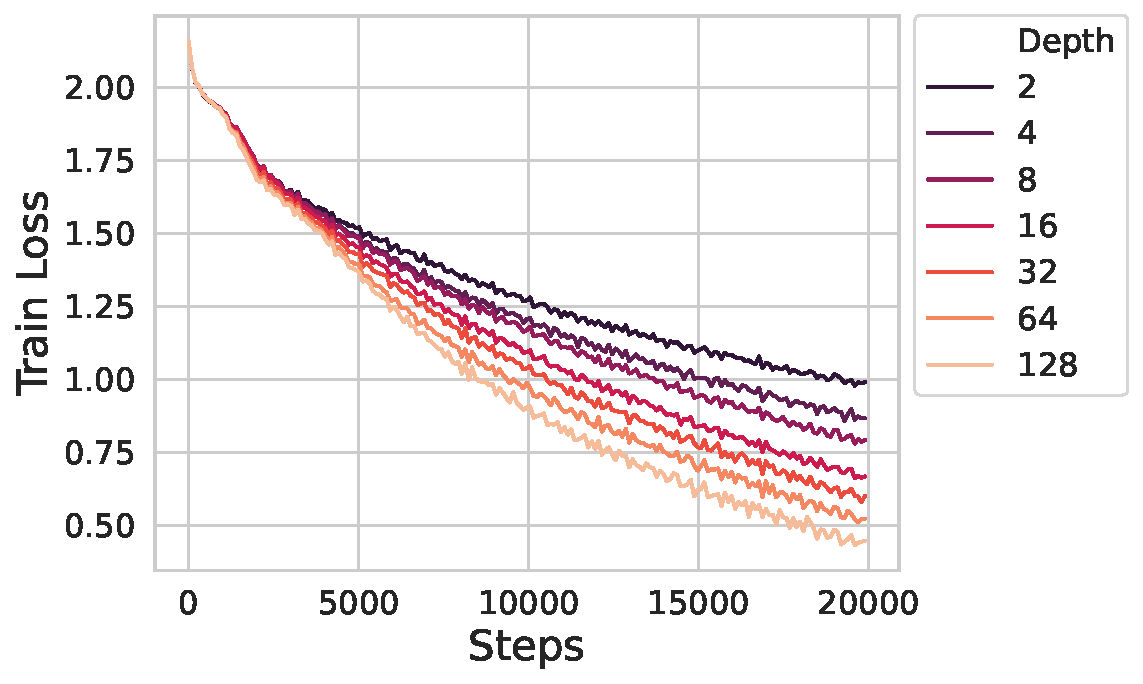
\includegraphics[width=0.4\linewidth]{figures/ODE_zero_init_loss_curves_1.pdf}}
    \subfigure[ODE $\frac{1}{L}$ Transfer]{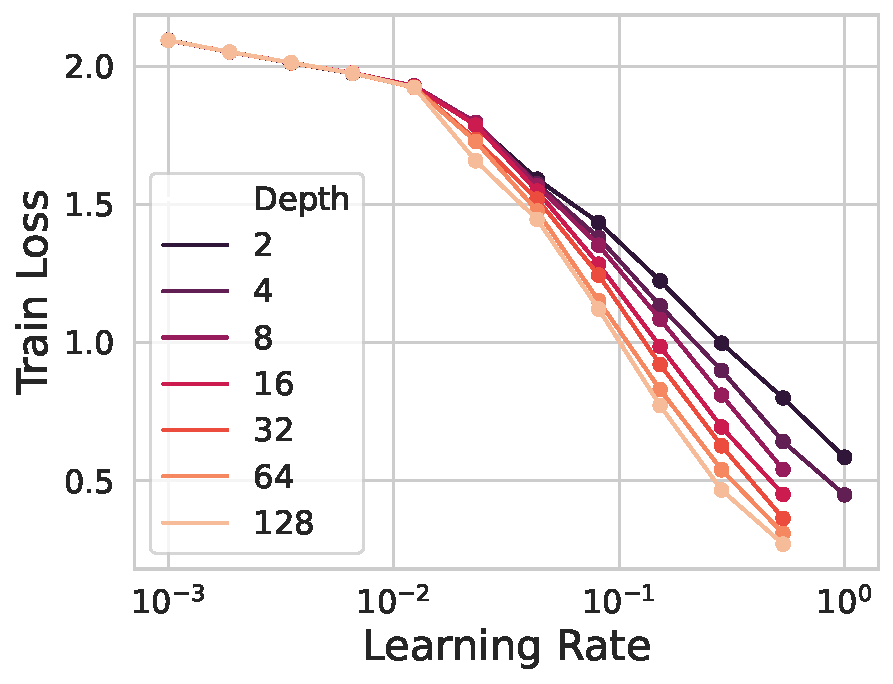
\includegraphics[width=0.32\linewidth]{figures/ODE_zero_init_LR_transfer_curves.pdf}}
    \subfigure[SDE $\frac{1}{\sqrt L}$ Dynamics]{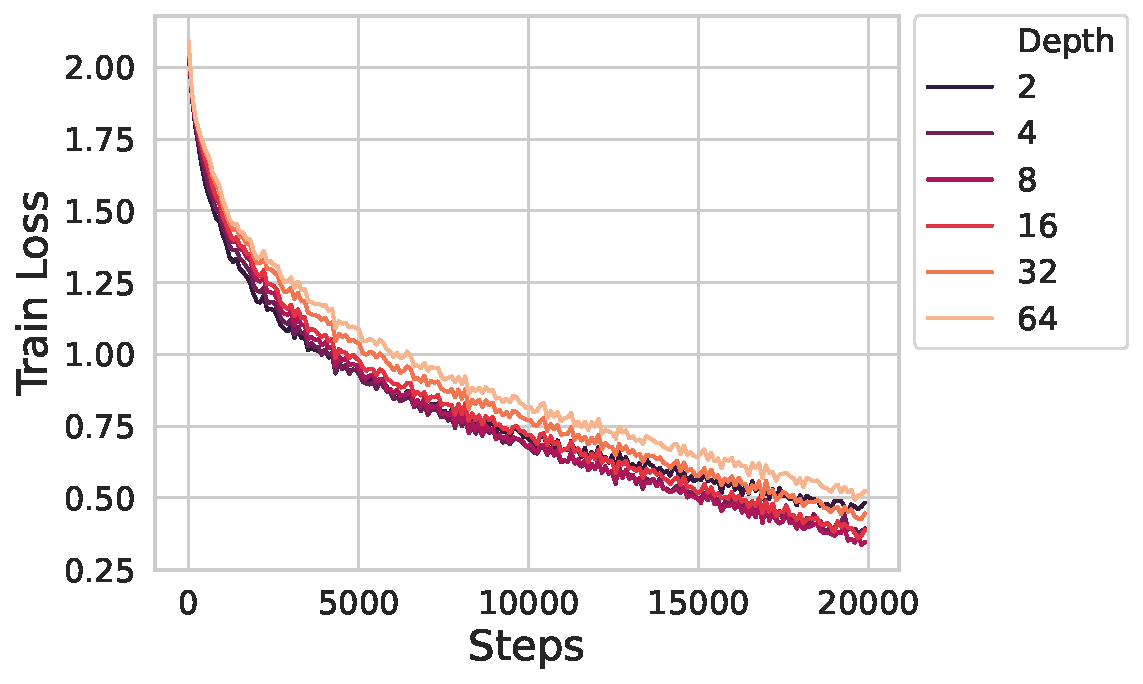
\includegraphics[width=0.4\linewidth]{figures/SDE_zero_init_loss_curves_1.pdf}}
    \subfigure[SDE $\frac{1}{\sqrt L}$ Transfer]{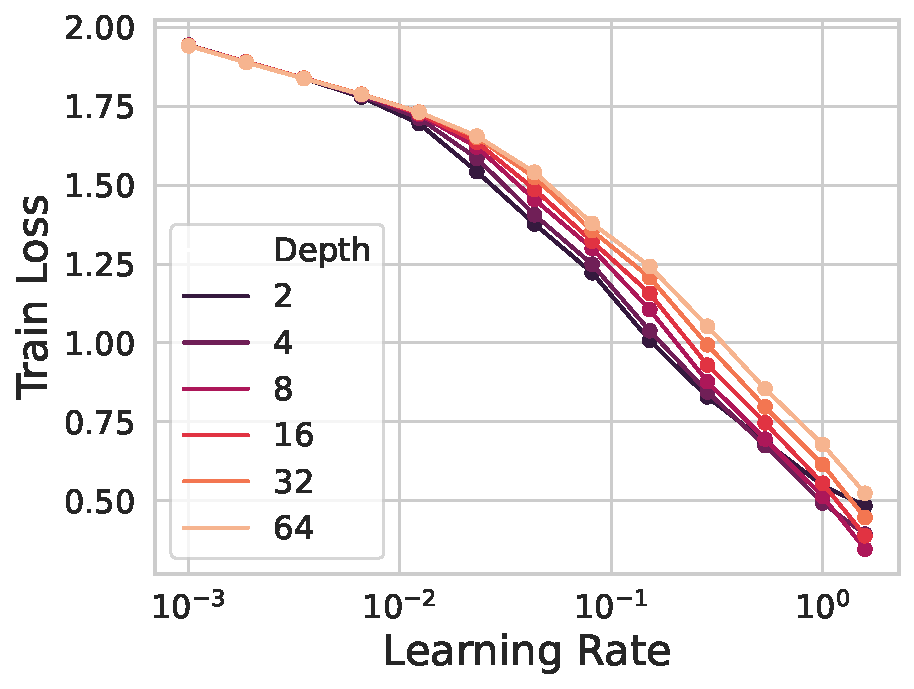
\includegraphics[width=0.32\linewidth]{figures/SDE_zero_init_LR_transfer_curves.pdf}}
    \caption{Hyperparameters transfer for both SDE and ODE scalings for multi-layer-per-block model $K=4$ models. Depth $L$ is varied for both models. Increasing $L$ leads to monotone improvements in the ODE but not SDE when initializing with zero readout weights for each block. In (d) all runs diverge at the next biggest learning rate.  }
    \label{fig:SDE_vs_ODE_K4}
\end{figure}

A more in-depth characterization of the differences in transferability and convergence rates of models in each of these parameterizations will be left to future work. 


%\subsection{Adam}

%\bb{TODO}

%\subsection{LayerNorm}

%\bb{TODO}


% \section{Submission of conference papers to ICLR 2024}

% ICLR requires electronic submissions, processed by
% \url{https://openreview.net/}. See ICLR's website for more instructions.

% If your paper is ultimately accepted, the statement {\tt
%   {\textbackslash}iclrfinalcopy} should be inserted to adjust the
% format to the camera ready requirements.

% The format for the submissions is a variant of the NeurIPS format.
% Please read carefully the instructions below, and follow them
% faithfully.

% \subsection{Style}

% Papers to be submitted to ICLR 2024 must be prepared according to the
% instructions presented here.

% %% Please note that we have introduced automatic line number generation
% %% into the style file for \LaTeXe. This is to help reviewers
% %% refer to specific lines of the paper when they make their comments. Please do
% %% NOT refer to these line numbers in your paper as they will be removed from the
% %% style file for the final version of accepted papers.

% Authors are required to use the ICLR \LaTeX{} style files obtainable at the
% ICLR website. Please make sure you use the current files and
% not previous versions. Tweaking the style files may be grounds for rejection.

% \subsection{Retrieval of style files}

% The style files for ICLR and other conference information are available online at:
% \begin{center}
%    \url{http://www.iclr.cc/}
% \end{center}
% The file \verb+iclr2024_conference.pdf+ contains these
% instructions and illustrates the
% various formatting requirements your ICLR paper must satisfy.
% Submissions must be made using \LaTeX{} and the style files
% \verb+iclr2024_conference.sty+ and \verb+iclr2024_conference.bst+ (to be used with \LaTeX{}2e). The file
% \verb+iclr2024_conference.tex+ may be used as a ``shell'' for writing your paper. All you
% have to do is replace the author, title, abstract, and text of the paper with
% your own.

% The formatting instructions contained in these style files are summarized in
% sections \ref{gen_inst}, \ref{headings}, and \ref{others} below.

% \section{General formatting instructions}
% \label{gen_inst}

% The text must be confined within a rectangle 5.5~inches (33~picas) wide and
% 9~inches (54~picas) long. The left margin is 1.5~inch (9~picas).
% Use 10~point type with a vertical spacing of 11~points. Times New Roman is the
% preferred typeface throughout. Paragraphs are separated by 1/2~line space,
% with no indentation.

% Paper title is 17~point, in small caps and left-aligned.
% All pages should start at 1~inch (6~picas) from the top of the page.

% Authors' names are
% set in boldface, and each name is placed above its corresponding
% address. The lead author's name is to be listed first, and
% the co-authors' names are set to follow. Authors sharing the
% same address can be on the same line.

% Please pay special attention to the instructions in section \ref{others}
% regarding figures, tables, acknowledgments, and references.


% There will be a strict upper limit of 9 pages for the main text of the initial submission, with unlimited additional pages for citations. 

% \section{Headings: first level}
% \label{headings}

% First level headings are in small caps,
% flush left and in point size 12. One line space before the first level
% heading and 1/2~line space after the first level heading.

% \subsection{Headings: second level}

% Second level headings are in small caps,
% flush left and in point size 10. One line space before the second level
% heading and 1/2~line space after the second level heading.

% \subsubsection{Headings: third level}

% Third level headings are in small caps,
% flush left and in point size 10. One line space before the third level
% heading and 1/2~line space after the third level heading.

% \section{Citations, figures, tables, references}
% \label{others}

% These instructions apply to everyone, regardless of the formatter being used.

% \subsection{Citations within the text}

% Citations within the text should be based on the \texttt{natbib} package
% and include the authors' last names and year (with the ``et~al.'' construct
% for more than two authors). When the authors or the publication are
% included in the sentence, the citation should not be in parenthesis using \verb|\citet{}| (as
% in ``See \citet{Hinton06} for more information.''). Otherwise, the citation
% should be in parenthesis using \verb|\citep{}| (as in ``Deep learning shows promise to make progress
% towards AI~\citep{Bengio+chapter2007}.'').

% The corresponding references are to be listed in alphabetical order of
% authors, in the \textsc{References} section. As to the format of the
% references themselves, any style is acceptable as long as it is used
% consistently.

% \subsection{Footnotes}

% Indicate footnotes with a number\footnote{Sample of the first footnote} in the
% text. Place the footnotes at the bottom of the page on which they appear.
% Precede the footnote with a horizontal rule of 2~inches
% (12~picas).\footnote{Sample of the second footnote}

% \subsection{Figures}

% All artwork must be neat, clean, and legible. Lines should be dark
% enough for purposes of reproduction; art work should not be
% hand-drawn. The figure number and caption always appear after the
% figure. Place one line space before the figure caption, and one line
% space after the figure. The figure caption is lower case (except for
% first word and proper nouns); figures are numbered consecutively.

% Make sure the figure caption does not get separated from the figure.
% Leave sufficient space to avoid splitting the figure and figure caption.

% You may use color figures.
% However, it is best for the
% figure captions and the paper body to make sense if the paper is printed
% either in black/white or in color.
% \begin{figure}[h]
% \begin{center}
% %\framebox[4.0in]{$\;$}
% \fbox{\rule[-.5cm]{0cm}{4cm} \rule[-.5cm]{4cm}{0cm}}
% \end{center}
% \caption{Sample figure caption.}
% \end{figure}

% \subsection{Tables}

% All tables must be centered, neat, clean and legible. Do not use hand-drawn
% tables. The table number and title always appear before the table. See
% Table~\ref{sample-table}.

% Place one line space before the table title, one line space after the table
% title, and one line space after the table. The table title must be lower case
% (except for first word and proper nouns); tables are numbered consecutively.

% \begin{table}[t]
% \caption{Sample table title}
% \label{sample-table}
% \begin{center}
% \begin{tabular}{ll}
% \multicolumn{1}{c}{\bf PART}  &\multicolumn{1}{c}{\bf DESCRIPTION}
% \\ \hline \\
% Dendrite         &Input terminal \\
% Axon             &Output terminal \\
% Soma             &Cell body (contains cell nucleus) \\
% \end{tabular}
% \end{center}
% \end{table}

% \section{Default Notation}

% In an attempt to encourage standardized notation, we have included the
% notation file from the textbook, \textit{Deep Learning}
% \cite{goodfellow2016deep} available at
% \url{https://github.com/goodfeli/dlbook_notation/}.  Use of this style
% is not required and can be disabled by commenting out
% \texttt{math\_commands.tex}.


% \centerline{\bf Numbers and Arrays}
% \bgroup
% \def\arraystretch{1.5}
% \begin{tabular}{p{1in}p{3.25in}}
% $\displaystyle a$ & A scalar (integer or real)\\
% $\displaystyle \va$ & A vector\\
% $\displaystyle \mA$ & A matrix\\
% $\displaystyle \tA$ & A tensor\\
% $\displaystyle \mI_n$ & Identity matrix with $n$ rows and $n$ columns\\
% $\displaystyle \mI$ & Identity matrix with dimensionality implied by context\\
% $\displaystyle \ve^{(i)}$ & Standard basis vector $[0,\dots,0,1,0,\dots,0]$ with a 1 at position $i$\\
% $\displaystyle \text{diag}(\va)$ & A square, diagonal matrix with diagonal entries given by $\va$\\
% $\displaystyle \ra$ & A scalar random variable\\
% $\displaystyle \rva$ & A vector-valued random variable\\
% $\displaystyle \rmA$ & A matrix-valued random variable\\
% \end{tabular}
% \egroup
% \vspace{0.25cm}

% \centerline{\bf Sets and Graphs}
% \bgroup
% \def\arraystretch{1.5}

% \begin{tabular}{p{1.25in}p{3.25in}}
% $\displaystyle \sA$ & A set\\
% $\displaystyle \R$ & The set of real numbers \\
% $\displaystyle \{0, 1\}$ & The set containing 0 and 1 \\
% $\displaystyle \{0, 1, \dots, n \}$ & The set of all integers between $0$ and $n$\\
% $\displaystyle [a, b]$ & The real interval including $a$ and $b$\\
% $\displaystyle (a, b]$ & The real interval excluding $a$ but including $b$\\
% $\displaystyle \sA \backslash \sB$ & Set subtraction, i.e., the set containing the elements of $\sA$ that are not in $\sB$\\
% $\displaystyle \gG$ & A graph\\
% $\displaystyle \parents_\gG(\ervx_i)$ & The parents of $\ervx_i$ in $\gG$
% \end{tabular}
% \vspace{0.25cm}


% \centerline{\bf Indexing}
% \bgroup
% \def\arraystretch{1.5}

% \begin{tabular}{p{1.25in}p{3.25in}}
% $\displaystyle \eva_i$ & Element $i$ of vector $\va$, with indexing starting at 1 \\
% $\displaystyle \eva_{-i}$ & All elements of vector $\va$ except for element $i$ \\
% $\displaystyle \emA_{i,j}$ & Element $i, j$ of matrix $\mA$ \\
% $\displaystyle \mA_{i, :}$ & Row $i$ of matrix $\mA$ \\
% $\displaystyle \mA_{:, i}$ & Column $i$ of matrix $\mA$ \\
% $\displaystyle \etA_{i, j, k}$ & Element $(i, j, k)$ of a 3-D tensor $\tA$\\
% $\displaystyle \tA_{:, :, i}$ & 2-D slice of a 3-D tensor\\
% $\displaystyle \erva_i$ & Element $i$ of the random vector $\rva$ \\
% \end{tabular}
% \egroup
% \vspace{0.25cm}


% \centerline{\bf Calculus}
% \bgroup
% \def\arraystretch{1.5}
% \begin{tabular}{p{1.25in}p{3.25in}}
% % NOTE: the [2ex] on the next line adds extra height to that row of the table.
% % Without that command, the fraction on the first line is too tall and collides
% % with the fraction on the second line.
% $\displaystyle\frac{d y} {d x}$ & Derivative of $y$ with respect to $x$\\ [2ex]
% $\displaystyle \frac{\partial y} {\partial x} $ & Partial derivative of $y$ with respect to $x$ \\
% $\displaystyle \nabla_\vx y $ & Gradient of $y$ with respect to $\vx$ \\
% $\displaystyle \nabla_\mX y $ & Matrix derivatives of $y$ with respect to $\mX$ \\
% $\displaystyle \nabla_\tX y $ & Tensor containing derivatives of $y$ with respect to $\tX$ \\
% $\displaystyle \frac{\partial f}{\partial \vx} $ & Jacobian matrix $\mJ \in \R^{m\times n}$ of $f: \R^n \rightarrow \R^m$\\
% $\displaystyle \nabla_\vx^2 f(\vx)\text{ or }\mH( f)(\vx)$ & The Hessian matrix of $f$ at input point $\vx$\\
% $\displaystyle \int f(\vx) d\vx $ & Definite integral over the entire domain of $\vx$ \\
% $\displaystyle \int_\sS f(\vx) d\vx$ & Definite integral with respect to $\vx$ over the set $\sS$ \\
% \end{tabular}
% \egroup
% \vspace{0.25cm}

% \centerline{\bf Probability and Information Theory}
% \bgroup
% \def\arraystretch{1.5}
% \begin{tabular}{p{1.25in}p{3.25in}}
% $\displaystyle P(\ra)$ & A probability distribution over a discrete variable\\
% $\displaystyle p(\ra)$ & A probability distribution over a continuous variable, or over
% a variable whose type has not been specified\\
% $\displaystyle \ra \sim P$ & Random variable $\ra$ has distribution $P$\\% so thing on left of \sim should always be a random variable, with name beginning with \r
% $\displaystyle  \E_{\rx\sim P} [ f(x) ]\text{ or } \E f(x)$ & Expectation of $f(x)$ with respect to $P(\rx)$ \\
% $\displaystyle \Var(f(x)) $ &  Variance of $f(x)$ under $P(\rx)$ \\
% $\displaystyle \Cov(f(x),g(x)) $ & Covariance of $f(x)$ and $g(x)$ under $P(\rx)$\\
% $\displaystyle H(\rx) $ & Shannon entropy of the random variable $\rx$\\
% $\displaystyle \KL ( P \Vert Q ) $ & Kullback-Leibler divergence of P and Q \\
% $\displaystyle \mathcal{N} ( \vx ; \vmu , \mSigma)$ & Gaussian distribution %
% over $\vx$ with mean $\vmu$ and covariance $\mSigma$ \\
% \end{tabular}
% \egroup
% \vspace{0.25cm}

% \centerline{\bf Functions}
% \bgroup
% \def\arraystretch{1.5}
% \begin{tabular}{p{1.25in}p{3.25in}}
% $\displaystyle f: \sA \rightarrow \sB$ & The function $f$ with domain $\sA$ and range $\sB$\\
% $\displaystyle f \circ g $ & Composition of the functions $f$ and $g$ \\
%   $\displaystyle f(\vx ; \vtheta) $ & A function of $\vx$ parameterized by $\vtheta$.
%   (Sometimes we write $f(\vx)$ and omit the argument $\vtheta$ to lighten notation) \\
% $\displaystyle \log x$ & Natural logarithm of $x$ \\
% $\displaystyle \sigma(x)$ & Logistic sigmoid, $\displaystyle \frac{1} {1 + \exp(-x)}$ \\
% $\displaystyle \zeta(x)$ & Softplus, $\log(1 + \exp(x))$ \\
% $\displaystyle || \vx ||_p $ & $\normlp$ norm of $\vx$ \\
% $\displaystyle || \vx || $ & $\normltwo$ norm of $\vx$ \\
% $\displaystyle x^+$ & Positive part of $x$, i.e., $\max(0,x)$\\
% $\displaystyle \1_\mathrm{condition}$ & is 1 if the condition is true, 0 otherwise\\
% \end{tabular}
% \egroup
% \vspace{0.25cm}



% \section{Final instructions}
% Do not change any aspects of the formatting parameters in the style files.
% In particular, do not modify the width or length of the rectangle the text
% should fit into, and do not change font sizes (except perhaps in the
% \textsc{References} section; see below). Please note that pages should be
% numbered.

% \section{Preparing PostScript or PDF files}

% Please prepare PostScript or PDF files with paper size ``US Letter'', and
% not, for example, ``A4''. The -t
% letter option on dvips will produce US Letter files.

% Consider directly generating PDF files using \verb+pdflatex+
% (especially if you are a MiKTeX user).
% PDF figures must be substituted for EPS figures, however.

% Otherwise, please generate your PostScript and PDF files with the following commands:
% \begin{verbatim}
% dvips mypaper.dvi -t letter -Ppdf -G0 -o mypaper.ps
% ps2pdf mypaper.ps mypaper.pdf
% \end{verbatim}

% \subsection{Margins in LaTeX}

% Most of the margin problems come from figures positioned by hand using
% \verb+\special+ or other commands. We suggest using the command
% \verb+\includegraphics+
% from the graphicx package. Always specify the figure width as a multiple of
% the line width as in the example below using .eps graphics
% \begin{verbatim}
%    \usepackage[dvips]{graphicx} ...
%    \includegraphics[width=0.8\linewidth]{myfile.eps}
% \end{verbatim}
% or % Apr 2009 addition
% \begin{verbatim}
%    \usepackage[pdftex]{graphicx} ...
%    \includegraphics[width=0.8\linewidth]{myfile.pdf}
% \end{verbatim}
% for .pdf graphics.
% See section~4.4 in the graphics bundle documentation (\url{http://www.ctan.org/tex-archive/macros/latex/required/graphics/grfguide.ps})

% A number of width problems arise when LaTeX cannot properly hyphenate a
% line. Please give LaTeX hyphenation hints using the \verb+\-+ command.

% \subsubsection*{Author Contributions}
% If you'd like to, you may include  a section for author contributions as is done
% in many journals. This is optional and at the discretion of the authors.

% \subsubsection*{Acknowledgments}
% Use unnumbered third level headings for the acknowledgments. All
% acknowledgments, including those to funding agencies, go at the end of the paper.


\end{document}
